\chapter{Resultados y discusión}
\lettrine{E}{}n la Sección \ref{Secc-ResultadosComposici} se muestran los resultados del análisis elemental de los seis núcleos sedimentarios de los  elementos mayoritarios: C, N, Na, Mg, Al, Si, S, Cl, K, Ca y Fe. El estudio de la fracción de la composición conocida indicó que en la mayoría de los núcleos sedimentarios se desconoce aproximadamente la mitad de la composición, salvo el núcleo sedimentario tipo manglar PCm en que se conoce el 74 \% de la composición. 
\\
\\
En la Sección \ref{Secc-EstimacionComposicion} se discute y se estandariza el porcentaje de oxígeno e hidrógeno para definir la composición corregida de cada sección de los núcleos sedimentarios. En la Sección \ref{Seccion-Correccion} se corrigen los perfiles de \PbCero\, debido a la composición y en la Sección \ref{Seccion-210y214} se discuten los perfiles corregidos de \PbCero, \PbCuatro\, y el equilibrio secular. 
\\
\\
El fechado mediante el modelo de Flujo Constante de los núcleos sedimentarios se describe en la Sección \ref{Seccion-Fechado} para los núcleos sedimentarios con una composición de referencia y una composición corregida, con un énfasis en la variabilidad de la eficiencia corregida y de las masas a lo largo del núcleo. 
	\section{Composición elemental de los núcleos sedimentarios}\label{Secc-ResultadosComposici}
Los resultados de la concentración a lo largo del núcleo de los ocho elementos de mayor concentración y la densidad promedio $\rho$ para los núcleos sedimentarios se muestran en la Tabla \ref{Tabla-ConcentracionDensidad} y en los diagramas de cajas de las Figuras \ref{Fig-ConcentracionNucleos1} - \ref{Fig-ConcentracionNucleos2}. Los extremos del intervalo de los diagramas de cajas corresponden a los valores de mínimo o máximo concentración, los extremos de la caja corresponden a los valores del primer y tercer cuartil, mientras el valor intermedio corresponde al segundo cuartil o mediana de la concentración a lo largo del núcleo.
\newpage
Las Figuras \ref{Fig-ConcentracionNucleos1} y \ref{Fig-ConcentracionNucleos2} muestran que la concentración absoluta de los elementos  de mayor contribución varía inter- e intra-núcleos. En relación con la variabilidad inter-núcleos, excepto para PCm, el elemento dominante promedio es el Si. El Si, como el Al, es habitualmente un indicador de las fuentes terrígenas \cite{Zabel2004}. Por otra parte, debido a que la península del Yucatán es una plataforma caliza, el núcleo sedimentario PCm no cuenta con Si ni Al entre los ocho elementos mayoritarios, es el único núcleo que presenta una contribución relevante de N (2 \%) y es el núcleo que presenta mayor contribución de C, 43 \% en promedio. Excluyendo este núcleo, todos los demás presentan una contribución promedio de C entre 3 \% - 12 \%. 
\\
\\
Por otro lado, salvo el núcleo sedimentario del lago de Santa María del Oro (SAMO-14-2), todos presentan una concentración relevante de Na y Cl, indicadores de fuentes marinas \cite{ruiz2016accretion}. El porcentaje promedio de la composición elemental conocida de los núcleos sedimentarios es menor al 50 \%, excepto para PCm (75 \%) y TEHUA-XII (66 \%). 
\\
\\
La variación de la composición intra-núcleos se evidencia en la dispersión de $\sum C$. La desviación estándar del promedio de la suma de los ocho elementos dominantes a lo largo de los núcleo PCm, LTAF y TEHUA-XII  es superior al 1 \%  (2\%, 14 \% y 7 \%, respectivamente). Los núcleos sedimentarios EU-VIII, GOMRI-500 y SAMO-14-2 presentan una desviación estándar menor que 1 \%, lo que sugiere la posibilidad de asumir una composición común para todas las secciones de estos núcleos.
\\
\\
La densidad promedio a lo largo de los núcleos sedimentarios (Tabla \ref{Tabla-ConcentracionDensidad}) se encuentra en un intervalo de 0.59 y 1.11 g cm$^{-3}$ y puede presentar variaciones a lo largo del mismo entre 0.11 g cm$^{-3}$ para GOMRI-500 hasta 0.43 g cm$^{-3}$ para LTAF. 
\begin{table}
\centering
\caption{Concentración absoluta promedio e intervalo de los ocho elementos de mayor contribución para cada núcleo sedimentario. Adicionalmente se muestra la suma de las concentraciones absolutas promedio medidas $\sum C$, y valor promedio $\overline{\rho}$, intervalo y variación $\bigtriangleup \rho$ de la densidad (en g cm$^{-3}$) a lo largo de los núcleos sedimentarios.}\label{Tabla-ConcentracionDensidad}
\begin{tabular}{|c|c|c|c|c|c|c|}\hline
\rowcolor{Blue3}	Elemento	&	EU-VIII	&	GOMRI-500	&	PCm	&	LTAF	&	SAMO-14-2	&	TEHUA-XII	\\ 	\hline	\hline
\rowcolor{Blue1}	C	&	0.07	&	0.03	&	0.43	&	0.12	&	0.08	&	0.06	\\ 		
\rowcolor{Blue1}		&	0.06-0.09	&	0.03-0.04	&	0.41-0.44	&	0.01-0.43	&	0.04-0.10	&	0.06-0.07	\\ 	\hline	
\rowcolor{Blue1}	N	&		&		&	0.02	&		&		&		\\ 		
\rowcolor{Blue1}		&		&		&	0.02-0.03	&		&		&		\\ 	\hline	
\rowcolor{Blue1}	Na	&	0.08	&	0.02	&	0.11	&	0.02	&		&	0.13	\\ 		
\rowcolor{Blue1}		&	0.07-0.09	&	0.01-0.03	&	0.07-0.14	&	0.01-0.04	&		&	0.09-0.17	\\ 	\hline	
\rowcolor{Blue1}	Mg	&		&		&	0.02	&	0.01	&	0.01	&	0.03	\\ 		
\rowcolor{Blue1}		&		&		&	0.01-0.03	&	0.01-0.01	&	0.00-0.01	&	0.02-0.04	\\ 	\hline	
\rowcolor{Blue1}	Al	&	0.07	&	0.07	&		&	0.06	&	0.04	&	0.09	\\ 		
\rowcolor{Blue1}		&	0.07-0.08	&	0.07-0.08	&		&	0.03-0.07	&	0.02-0.08	&	0.06-0.11	\\ 	\hline	
\rowcolor{Blue1}	Si	&	0.17	&	0.20	&		&	0.20	&	0.19	&	0.24	\\ 		
\rowcolor{Blue1}		&	0.16-0.18	&	0.18-0.23	&		&	0.08-0.23	&	0.16-0.27	&	0.18-0.28	\\ 	\hline	
\rowcolor{Blue1}	S 	&	0.03	&		&	0.04	&		&	0.01	&		\\ 		
\rowcolor{Blue1}		&	0.01-0.04	&		&	0.02-0.06	&		&	0.00-0.01	&		\\ 	\hline	
\rowcolor{Blue1}	Cl	&	0.05	&	0.02	&	0.11	&		&		&	0.06	\\ 		
\rowcolor{Blue1}		&	0.04-0.06	&	0.01-0.02	&	0.08-0.14	&		&		&	0.05-0.08	\\ 	\hline	
\rowcolor{Blue1}	K	&	0.02	&	0.02	&	0.002	&	0.02	&	0.01	&		\\ 		
\rowcolor{Blue1}		&	0.02-0.02	&	0.02-0.02	&	0.002-0.004	&	0.01-0.02	&	0.00-0.02	&		\\ 	\hline	
\rowcolor{Blue1}	Ca	&		&	0.07	&	0.01	&	0.01	&	0.12	&	0.03	\\ 		
\rowcolor{Blue1}		&		&	0.06-0.07	&	0.00-0.04	&	0.01-0.02	&	0.06-0.18	&	0.02-0.04	\\ 	\hline	
\rowcolor{Blue1}	Fe	&	0.03	&	0.03	&		&	0.04	&	0.02	&	0.03	\\ 		
\rowcolor{Blue1}		&	0.03-0.04	&	0.03-0.04	&		&	0.02-0.06	&	0.00-0.04	&	0.03-0.03	\\ 	\hline	\hline
\rowcolor{Blue2}	$\sum C$	&	0.53	&	0.46	&	0.74	&	0.48	&	0.47	&	0.66	\\ 	\hline	\hline
\rowcolor{Blue2}	$\overline{\rho}$	&	1.04	&	1.11	&	0.59	&	1.07	&	0.84	&	0.81	\\ 
\rowcolor{Blue2}	Intervalo de $\rho$	&	0.99-1.15	&	1.06-1.17	&	0.52-0.74	&	0.75-1.18	&	0.71-0.98	&	0.61-0.86	\\ 	
\rowcolor{Blue2}	 $\bigtriangleup \rho$ & 0.16	&	0.11	&	0.22	&	0.43	&	0.27	&	0.25 \\ \hline
\end{tabular}
\end{table}
\begin{figure}
\centering
\includegraphics[width=0.9\textwidth]{Imagenes/XRF_Todos_Los_Nucleos_1.png}
\caption{Diagrama de cajas de los núcleos sedimentarios EU-VIII, GOMRI-500 y PCm para los ochos elementos de mayor concentración. Para cada núcleo sedimentario se incluye el valor porcentual de la suma promedio de las concentraciones medidas $\sum C$.}\label{Fig-ConcentracionNucleos1}
\end{figure}
\begin{figure}
\centering
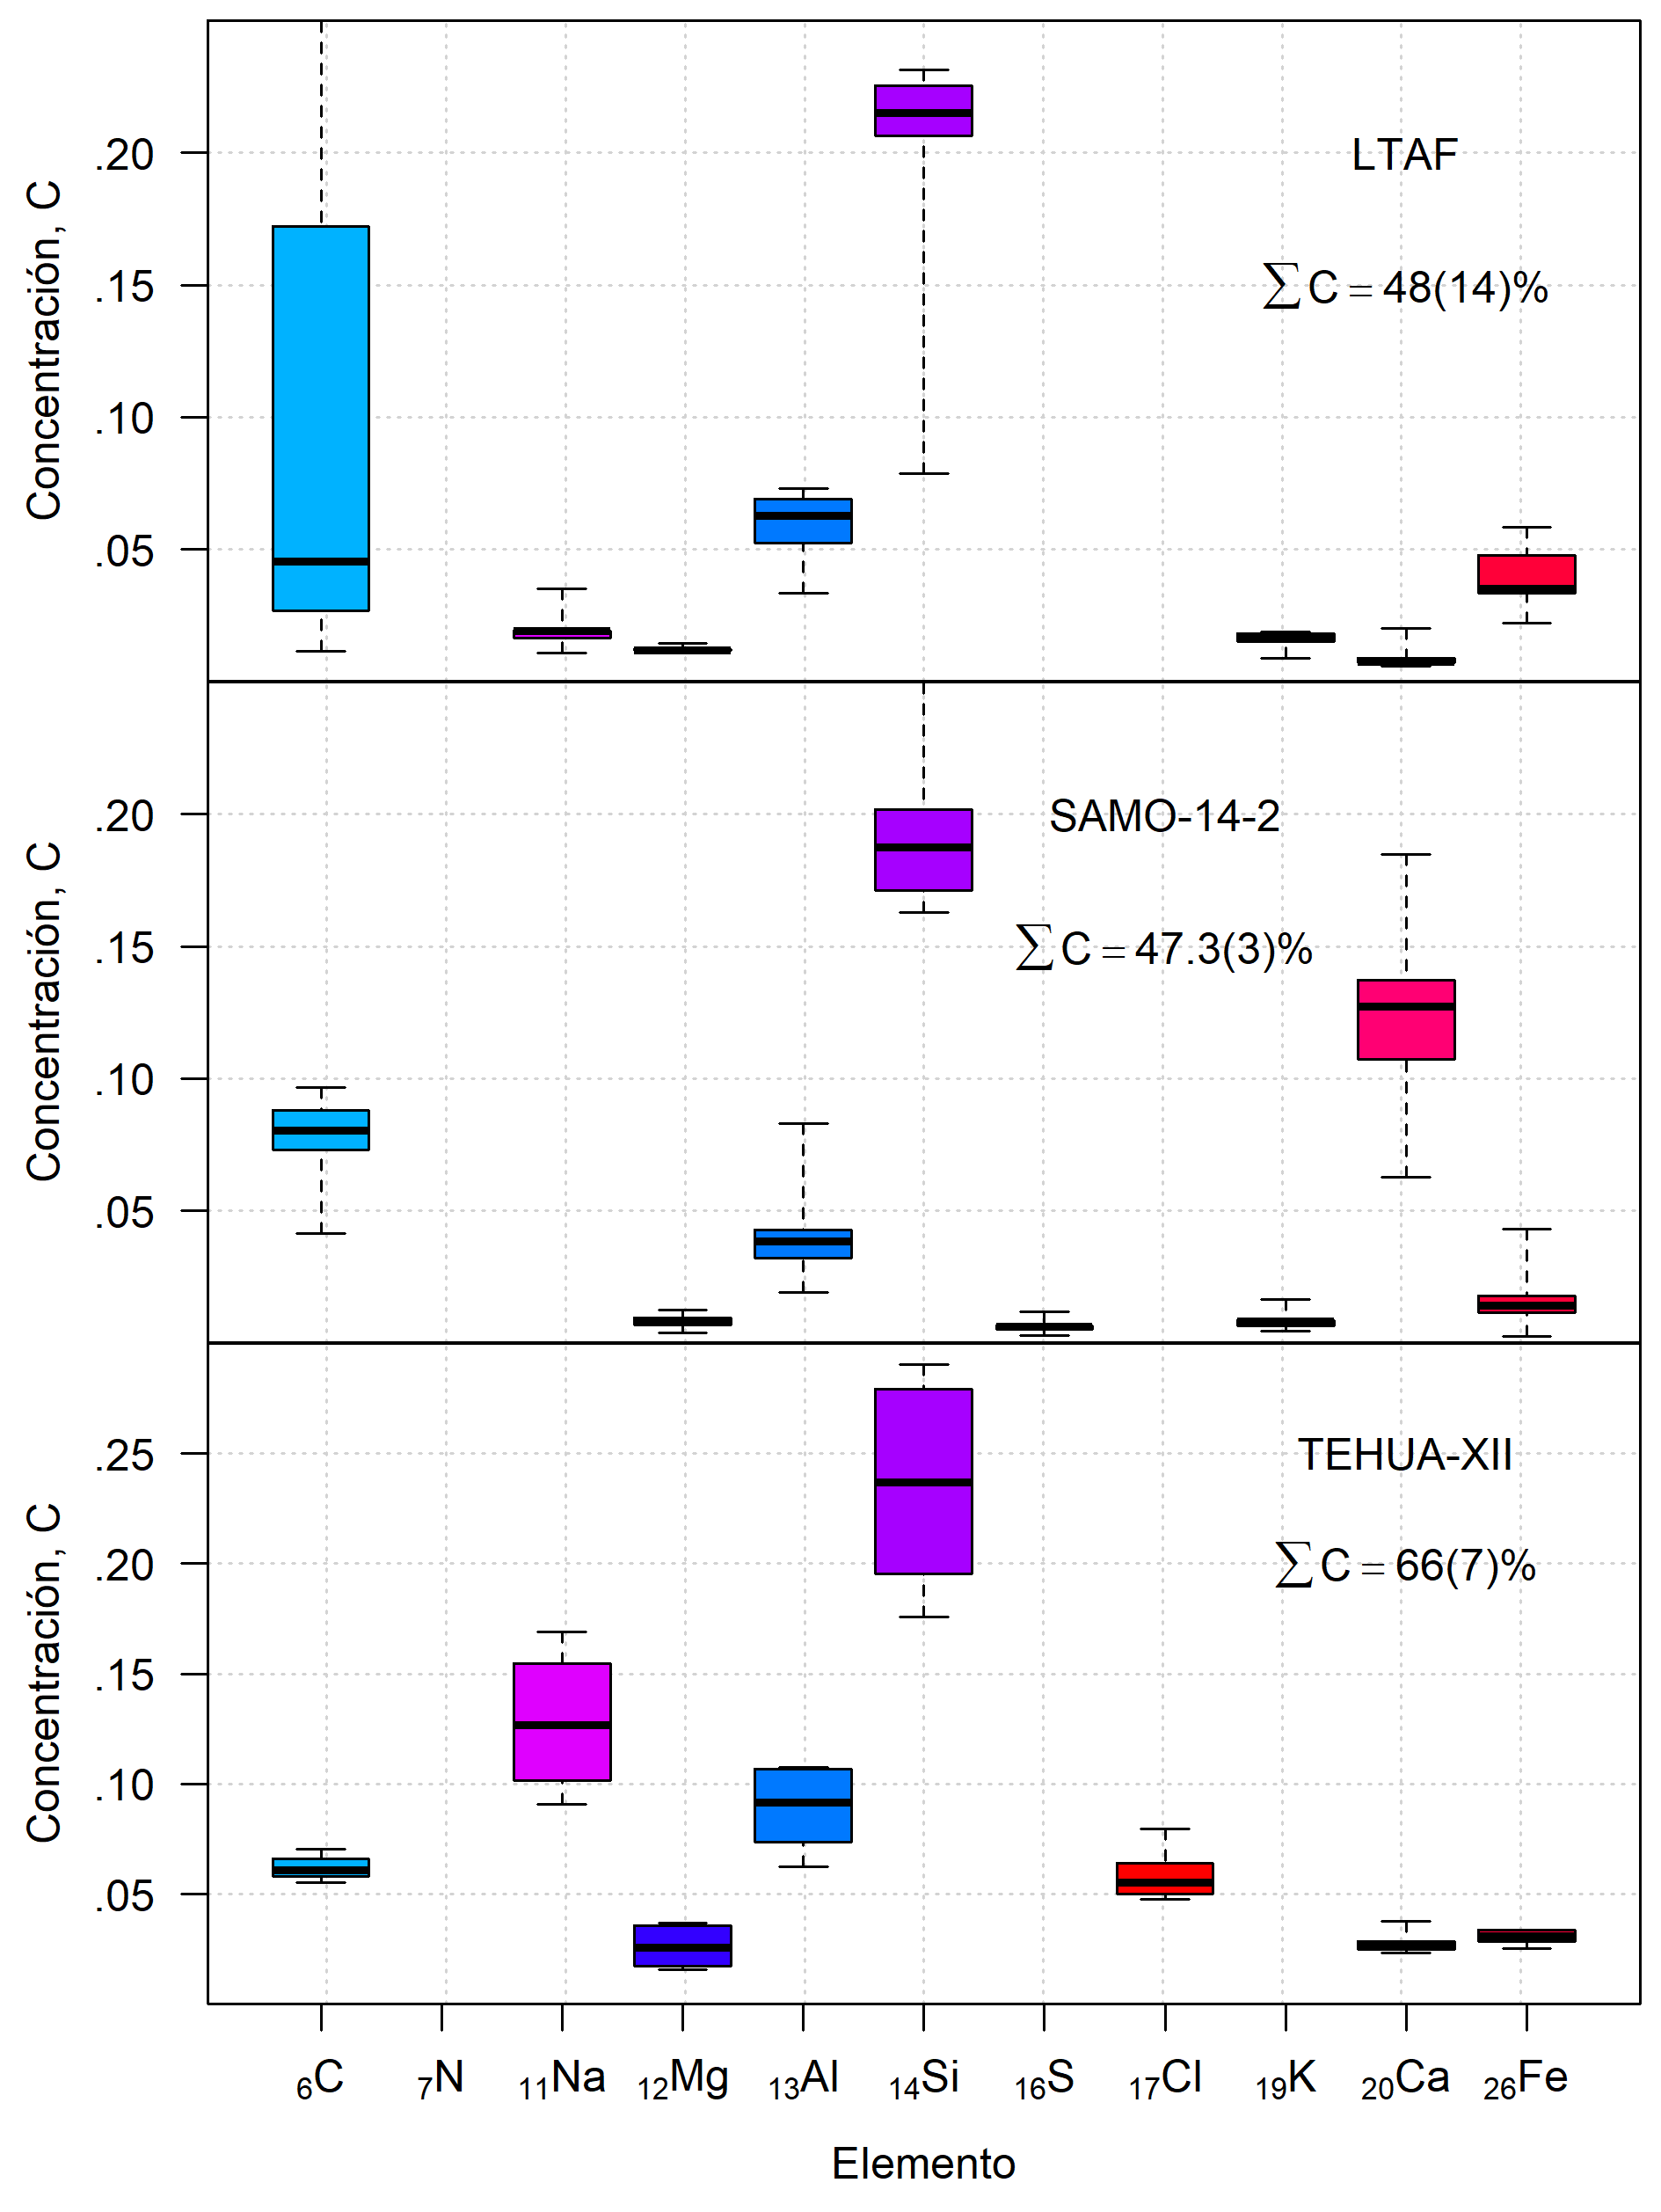
\includegraphics[width=0.9\textwidth]{Imagenes/XRF_Todos_Los_Nucleos_2.png}
\caption{Diagrama de cajas de los núcleos sedimentarios LTAF, SAMO-14-2 y TEHUA-XII para los ochos elementos de mayor concentración.  Para cada núcleo sedimentario se incluye el valor porcentual de la suma promedio de las concentraciones medidas $\sum C$.}\label{Fig-ConcentracionNucleos2}
\end{figure}
\newpage
	\section{Estimación de la composición desconocida}\label{Secc-EstimacionComposicion}
Una vez establecida la composición conocida, es necesario realizar una estimación de la composición desconocida de cada muestra. En la Tabla \ref{Tabla-Eficiencias} se muestran las diferencias porcentuales promedio de los valores de la eficiencia corregida para 46.54 keV respecto a la eficiencia de referencia para composiciones desconocidas de 0 \%, 50 \% y 100 \% de oxígeno. La variación porcentual promedio es del 3 \% para todos los núcleos sedimentarios analizados, y varía entre 0.8 \% y 4 \%. La incertidumbre típica de las actividades de \PbCero\, y \PbCuatro, medidas por espectrometría de rayos gamma, es típicamente mayor al 6 \%. Se consideró que el uso de una composición corregida con el 50 \% oxígeno en la fracción desconocida es aceptable porque la desviación promedio calculada (3 \%) es inferior a la incertidumbre de la medida.
\\
\\
Para los núcleos sedimentarios considerados, la corrección mínima realizada (1.7 \%, Tabla \ref{Tabla-Eficiencias}) fue para PCm. Efectivamente, el componente mayoritario de este núcleo es el átomo ligero C, con una atenuación por autoabsorción mínima, por lo que se podría asumir en este caso que la composición de referencia puede ser utilizada sin correcciones debido a la composición. Podemos concluir que para muestras con un alto contenido de materia orgánica, en general, no es necesario aplicar correcciones por autoabsorción.
\\ \\ 
En los otros casos, las diferencias promedio entre las eficiencias de referencia y corregida son relevantes, e ignorar su corrección puede inducir a errores substanciales en la cuantificación de las actividades de \PbCero\, en las muestras. En promedio, estos errores son aproximadamente del 10 \% para EU-VIII, LTAF, SAMO-14-2 y TEHUA-XII, y de 16 \% para GOMRI-500. Concluimos que la corrección por densidad y autoabsorción es necesaria cuando la determinación de la actividad absoluta de \PbCero\, es importante.
\begin{table}[h]
\centering
\caption{Diferencia porcentual promedio de las eficiencias para 46.54 keV respecto a la calibración de referencia para diferentes composiciones desconocidas de H y O.}\label{Tabla-Eficiencias}
\begin{tabular}{|c|c|c|c|c|}\hline
\rowcolor{Blue3}	Núcleo 	&	 \multicolumn{3}{c|}{Dif. porcentual promedio en $\epsilon$}           					&	Variación en Dif. 	\\ 	
\rowcolor{Blue3}	 sedimentario & \multicolumn{3}{c|}{$\overline{\epsilon} \pm \bigtriangleup \epsilon$}   & porcentuales \\	\hline
\rowcolor{Blue2}		&	0 \% Oxígeno 	&	\textbf{50 \% Oxígeno} 	&	100 \% Oxígeno 	&	0 \%  $\rightarrow$ 100 \% 	\\  \hline
\rowcolor{Blue1}	EU-VIII	&	$13 \pm 1$	&	$12 \pm 1$	&	$11 \pm 1$	&	2	\\ 	
\rowcolor{Blue1}	GOMRI-500	&	$18 \pm 1$	&	$16 \pm 1$	&	$14 \pm 1$	&	4	\\ 	
\rowcolor{Blue1}	PCm	&	$1.3 \pm 0.9$	&	$1.7 \pm 0.8$	&	$2.1 \pm 0.9$	&	0.8	\\ 	
\rowcolor{Blue1}	LTAF	&	$14 \pm 5$	&	$12 \pm 4$	&	$10 \pm 4$	&	4	\\ 	
\rowcolor{Blue1}	SAMO-14-2	&	$10 \pm 2$	&	$8.5 \pm 1.9$	&	$7 \pm 2$	&	3	\\ 	
\rowcolor{Blue1}	TEHUA-XIII	&	$9 \pm 1$	&	$8 \pm 2$	&	$7 \pm 2$	&	2	\\ 	\hline
\rowcolor{Blue2}	 & \multicolumn{3}{r|}{Promedio:} 							&	3	\\ 	\hline
\end{tabular}
\end{table}	
\newpage
	\section{Corrección de las actividades de \PbCero}\label{Seccion-Correccion}
Una vez se ha estimado la composición corregida de la muestra, se calcularon las eficiencias corregidas para cada una de las secciones medidas y se determinaron las actividades corregidas. Los perfiles de actividad específica de \PbCero, con una composición de referencia y corregida, y su diferencia porcentual, se presentan en las Figuras \ref{FigEUVIIIAgua}, \ref{FigGOMRI500Agua}, \ref{FigPCmAgua}, \ref{FigLTAFAgua}, \ref{FigSAMO142Agua} y \ref{FigTEHUAXIIAgua}. Los rangos de actividad específica y profundidad de los anterior perfiles varían entre núcleos sedimentarios.
\\
\\
En todos los casos, se confirmó la presencia de exceso porque todos los perfiles muestran un decrecimiento con la profundidad. En el caso de los núcleos EU-VIII, PCm y SAMO-14-2, las diferencias observadas entre los dos perfiles son pequeñas y los perfiles son similares, dentro de la banda de incertidumbre. 
\\
\\
Sin embargo, para los núcleos GOMRI-500 y TEHUA-XII (ambos de ambientes de mar abierto y con baja concentración de C) las diferencias de las actividades de \PbCero, debidas a las correcciones de composición y densidad, son significativas sobretodo en la parte superior del núcleo, que contiene la mayor parte del inventario de \PbCeroEx, por lo que \textit{a priori} es de esperar que sean los núcleos donde el fechado sea más afectado por estas correcciones.
\begin{figure}
\centering
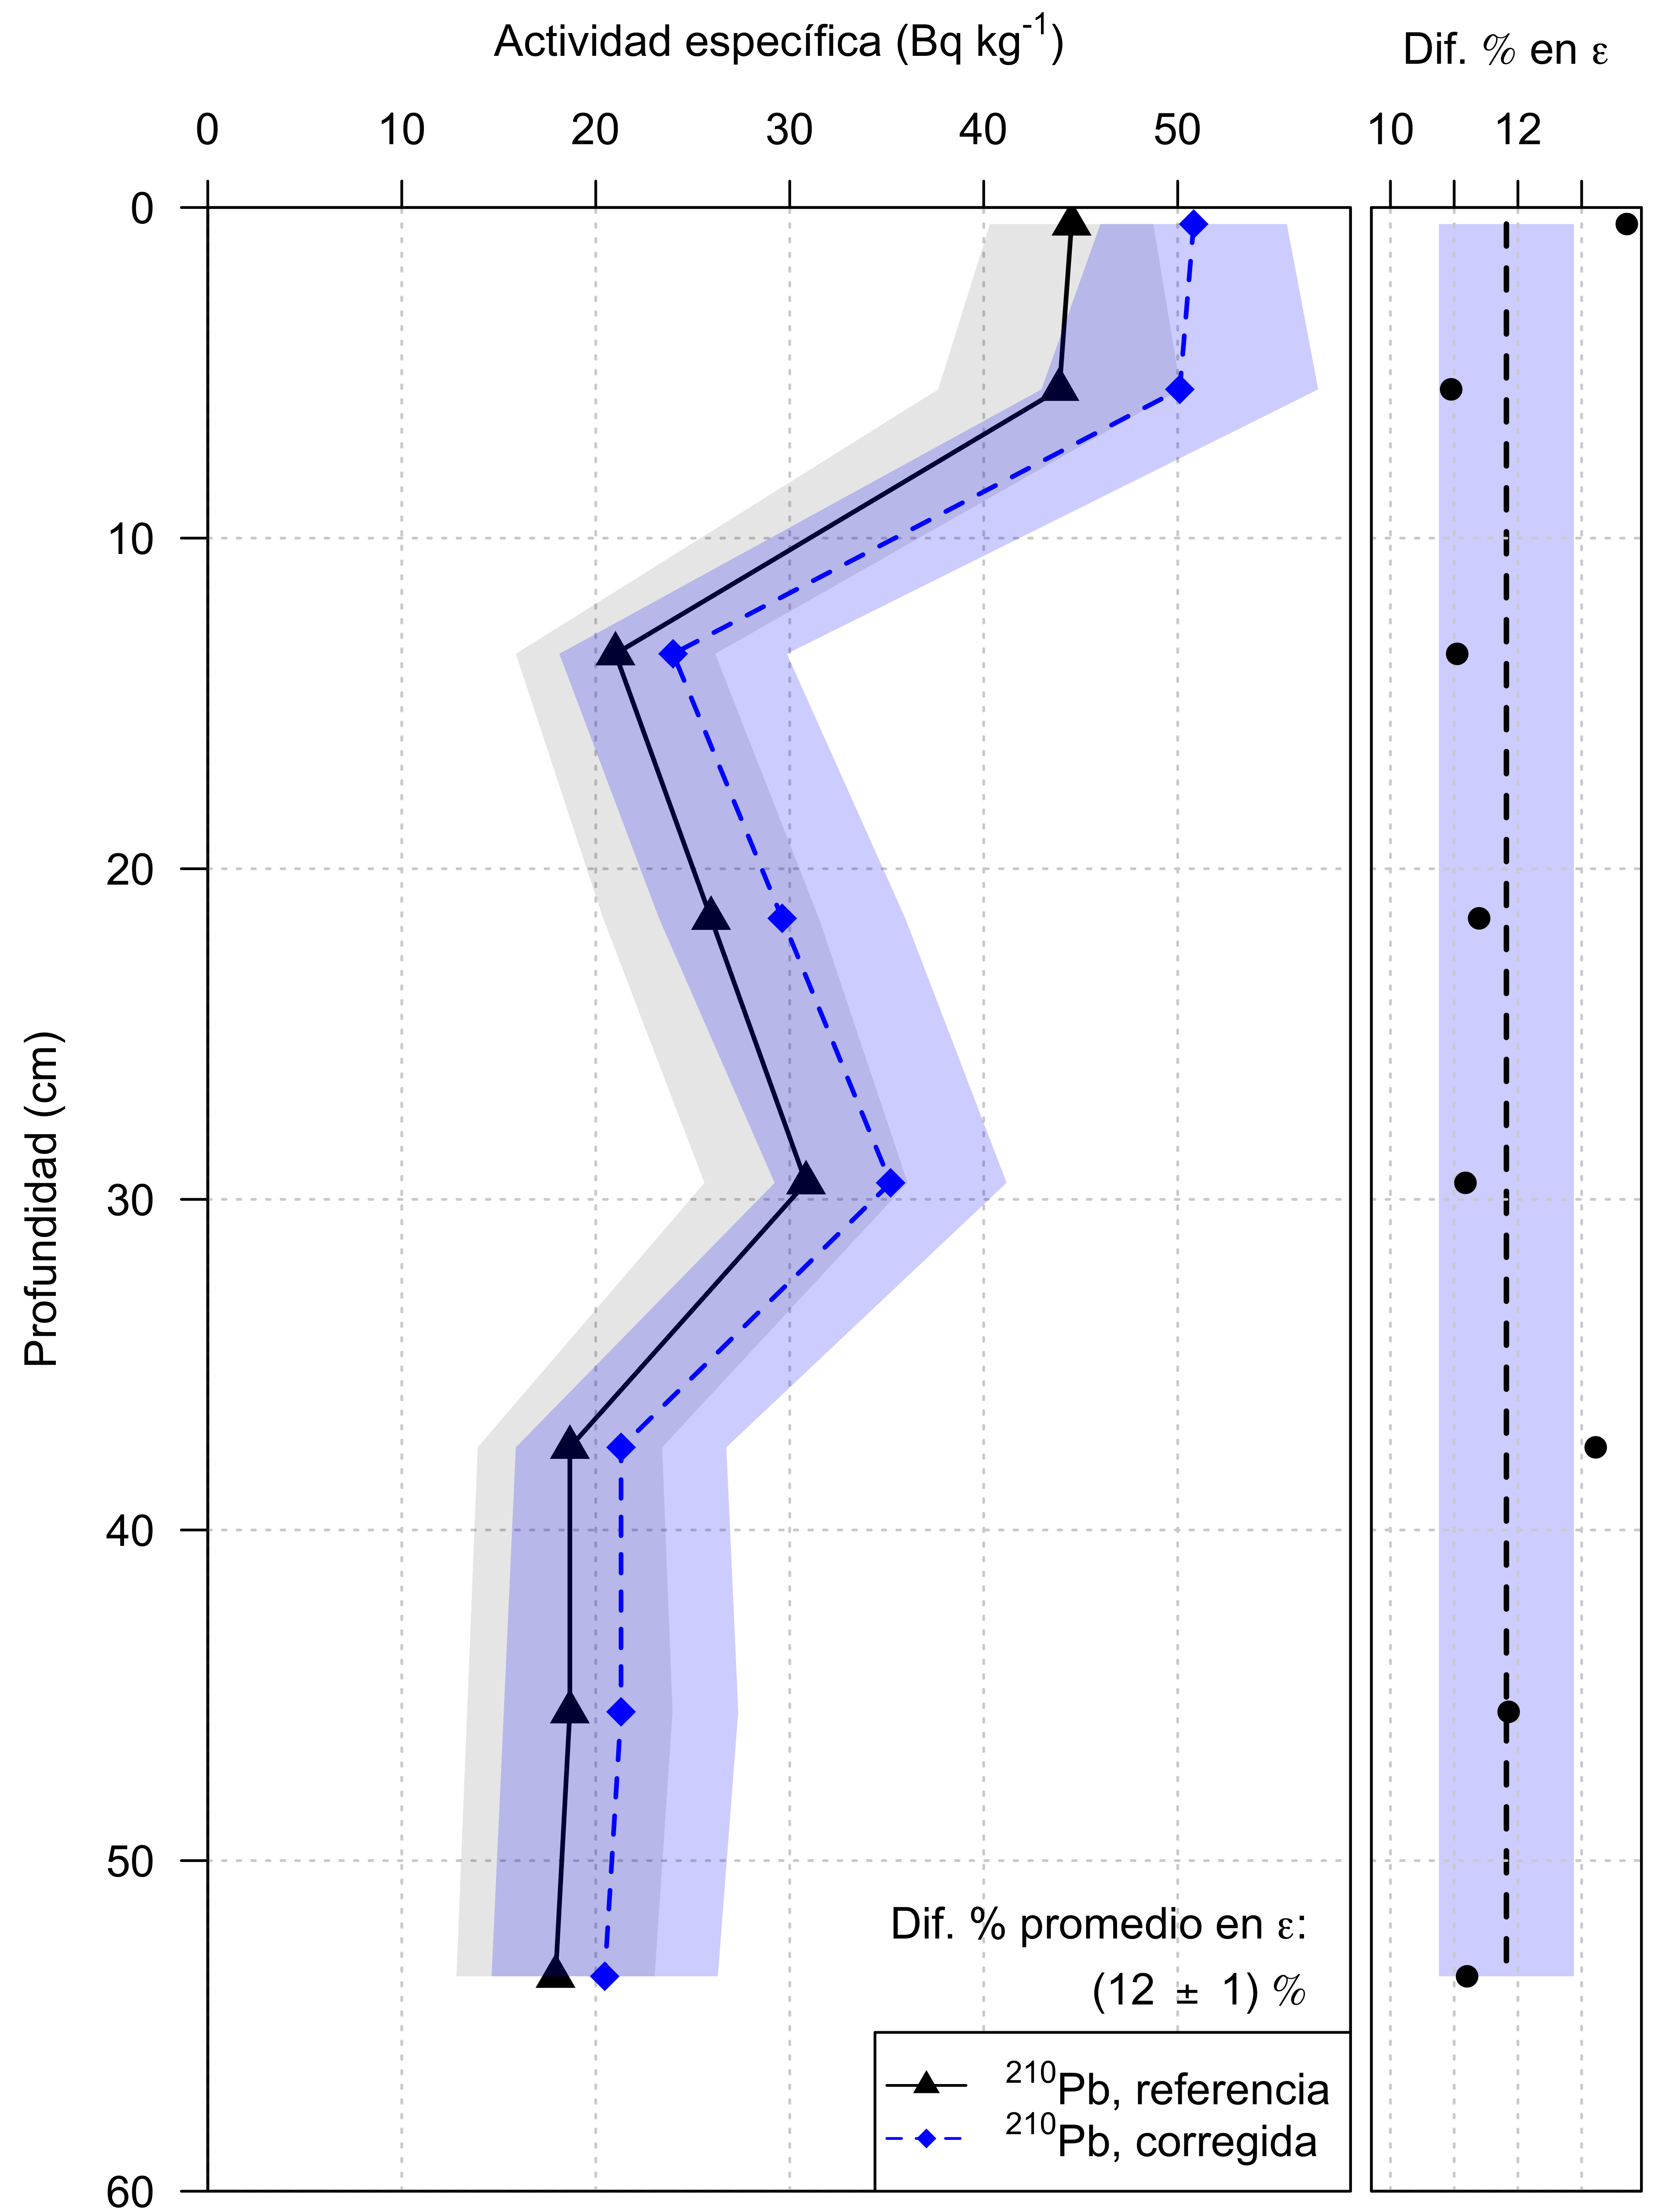
\includegraphics[width=0.9\textwidth]{Imagenes/Act_210Pb_Agua_Composicion_EU_VIII.png}
\caption{Perfil de actividad específica de \PbCero\, para el núcleo \textbf{EU-VIII} asumiendo una composición elemental de referencia y una composición corregida (Sección \ref{Secc-100Composicion}). Se muestra la diferencia porcentual promedio en el valor las eficiencias de referencia y corregida para una energía de 46.54 keV.}\label{FigEUVIIIAgua}
\end{figure}
\begin{figure}
\centering
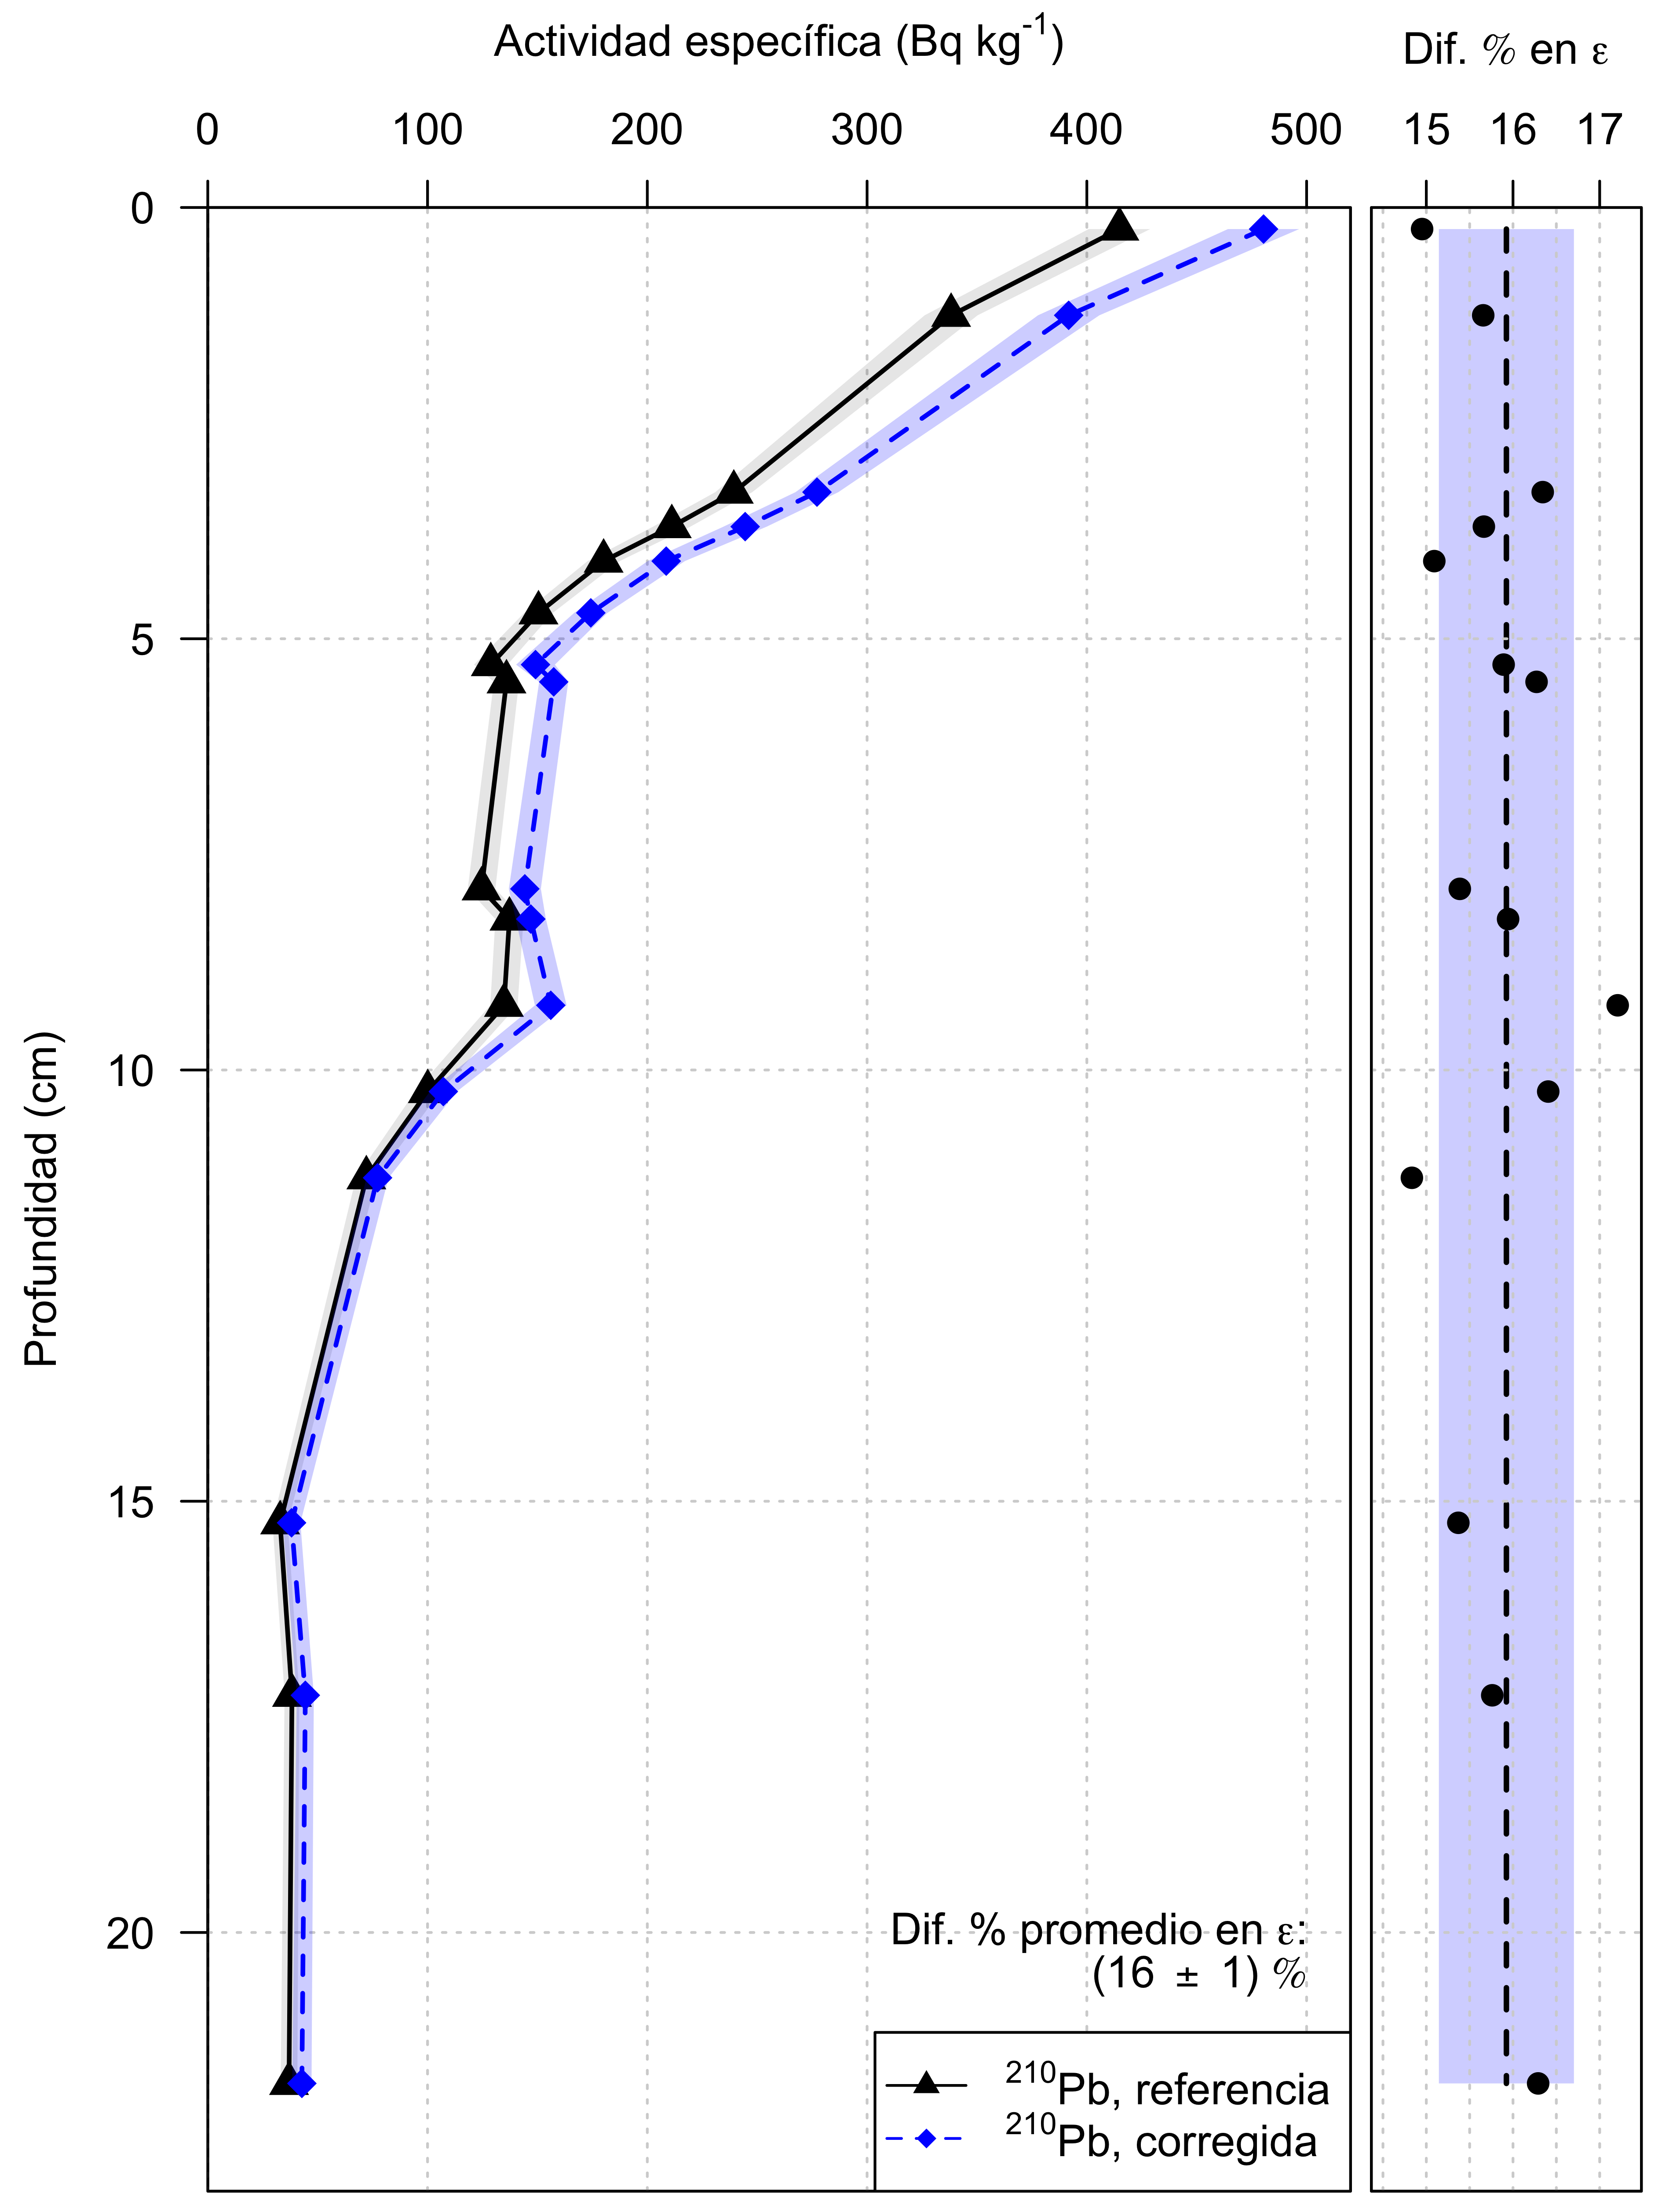
\includegraphics[width=0.9\textwidth]{Imagenes/Act_210Pb_Agua_Composicion_GOMRI_500.png}
\caption{Perfil de actividad específica de \PbCero\, para el núcleo \textbf{GOMRI-500} asumiendo una composición elemental de referencia y una composición corregida (Sección \ref{Secc-100Composicion}). Se muestra la diferencia porcentual promedio en el valor las eficiencias de referencia y corregida para una energía de 46.54 keV.}\label{FigGOMRI500Agua}
\end{figure}
\begin{figure}
\centering
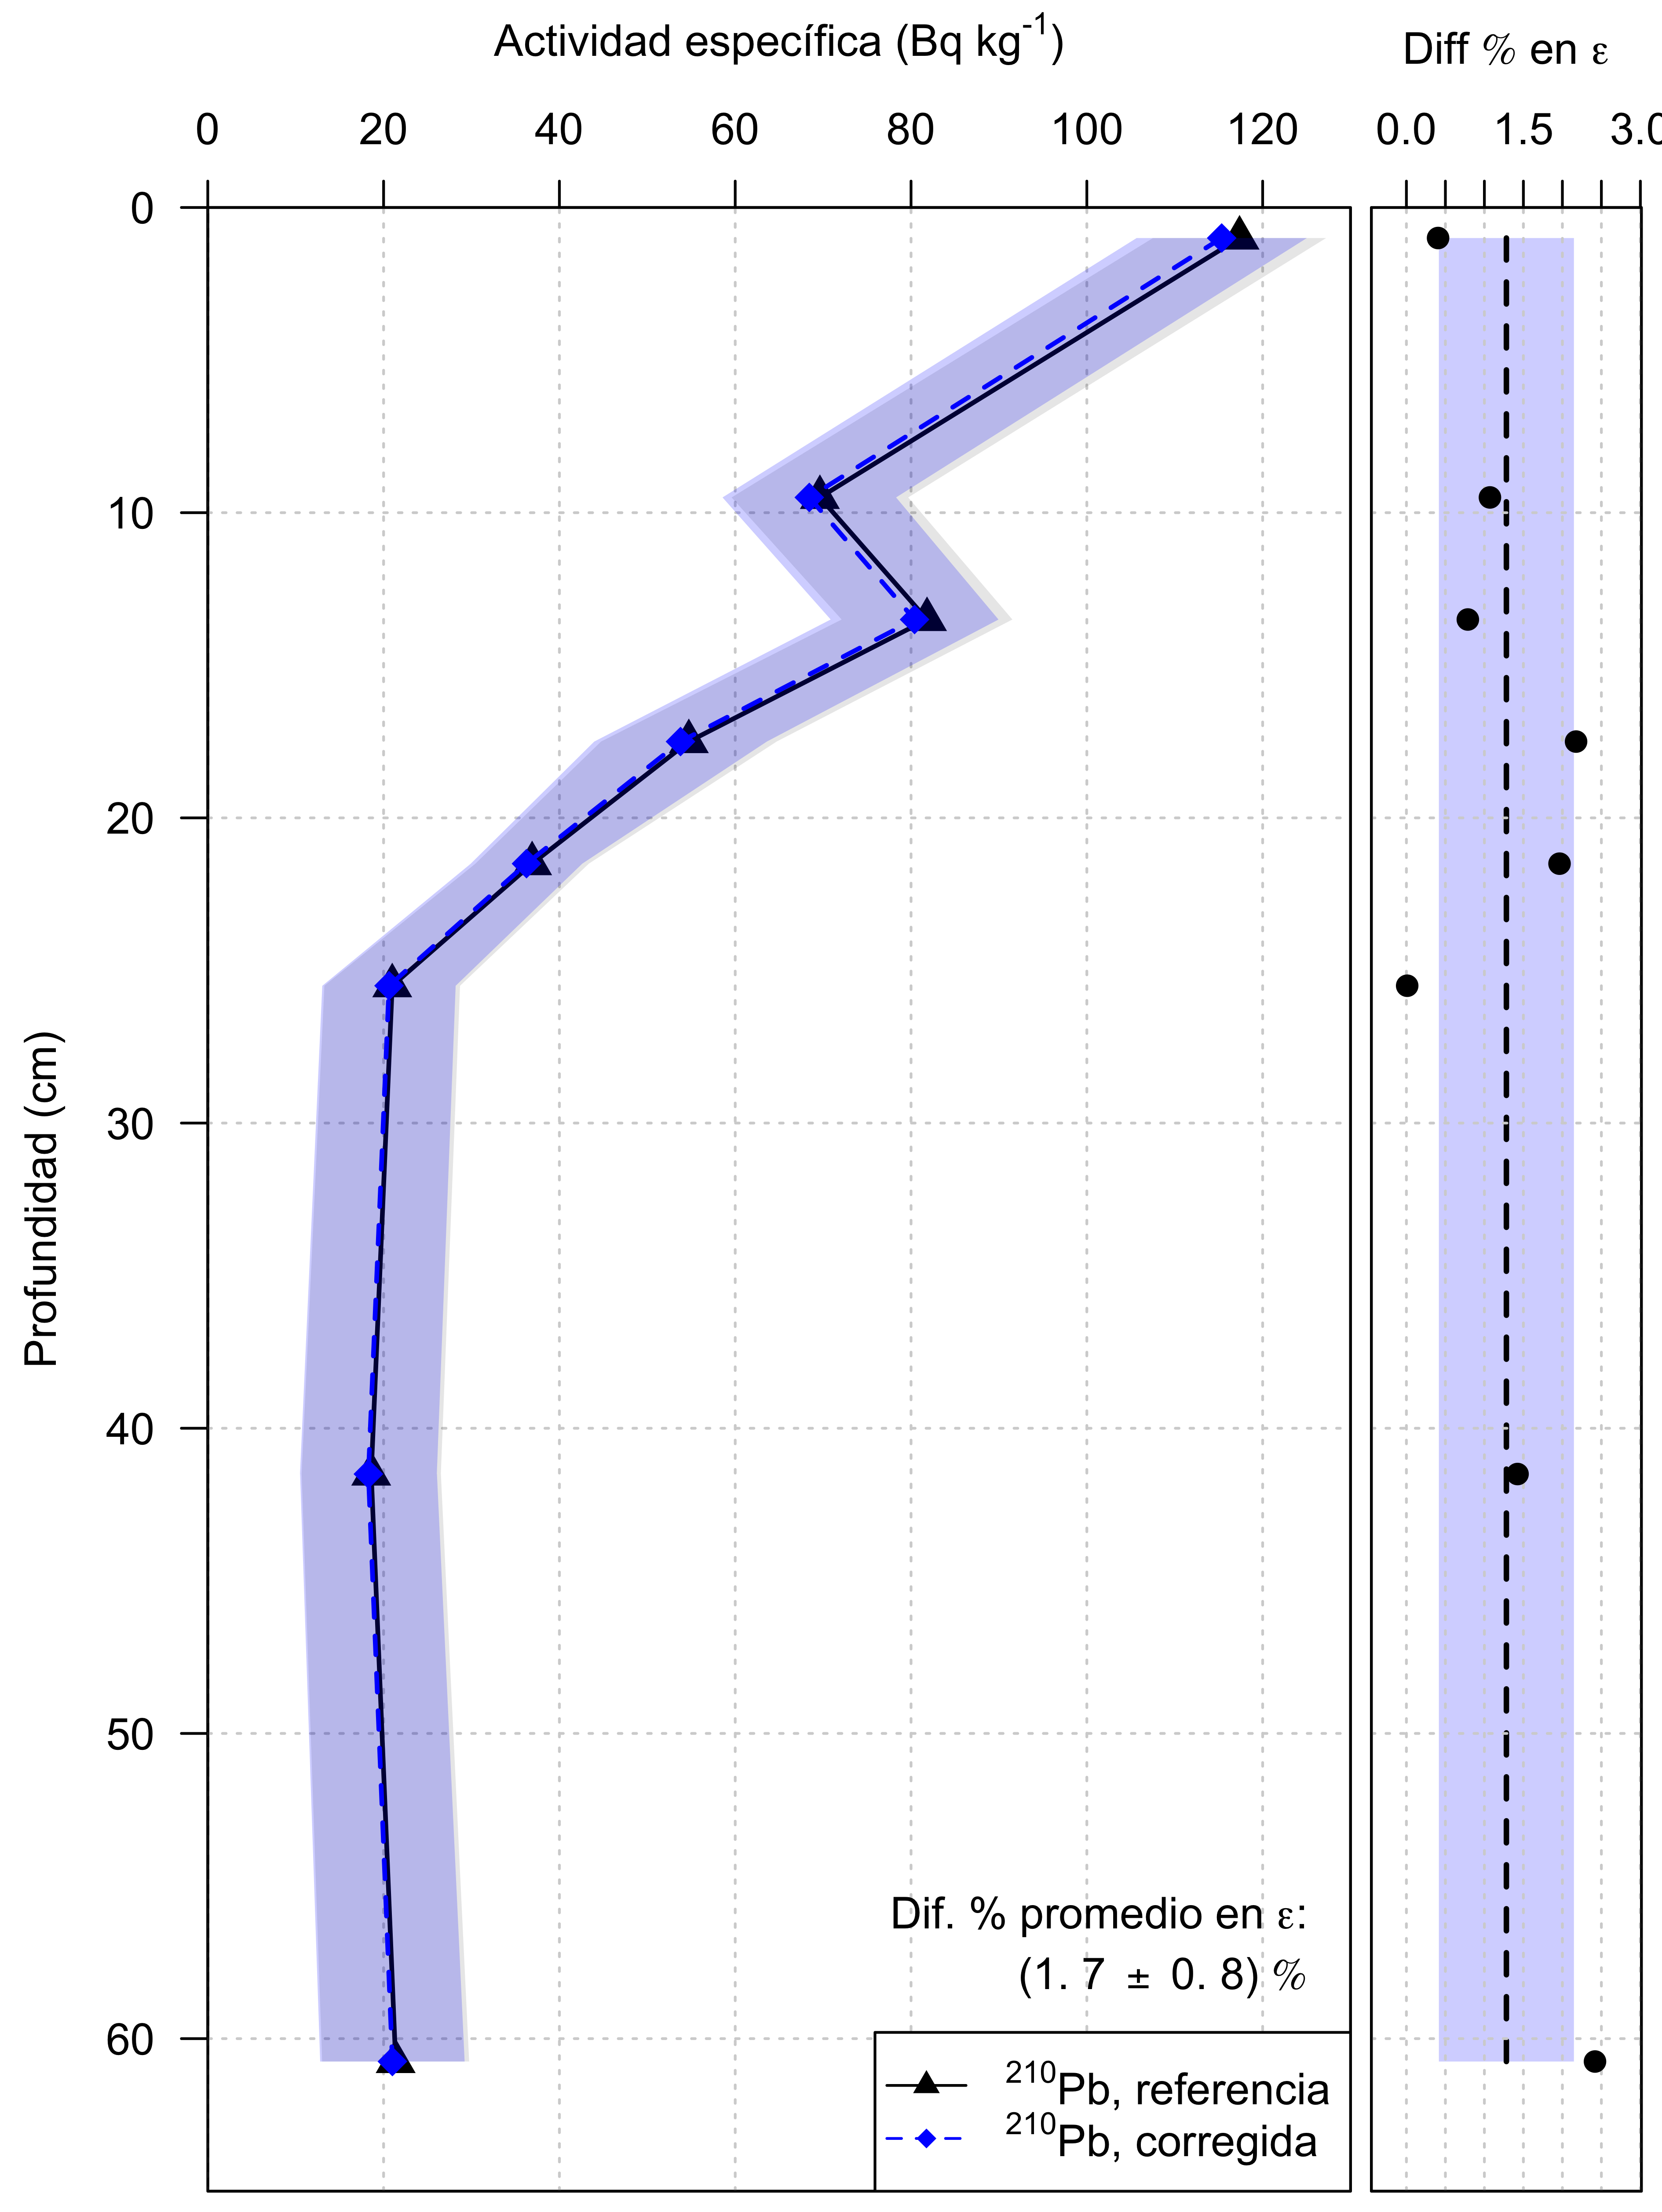
\includegraphics[width=0.9\textwidth]{Imagenes/Act_210Pb_Agua_Composicion_PCm.png}
\caption{Perfil de actividad específica de \PbCero\, para el núcleo \textbf{PCm} asumiendo una composición elemental de referencia y una composición corregida (Sección \ref{Secc-100Composicion}). Se muestra la diferencia porcentual promedio en el valor las eficiencias de referencia y corregida para una energía de 46.54 keV.}\label{FigPCmAgua}
\end{figure}
\begin{figure}
\centering
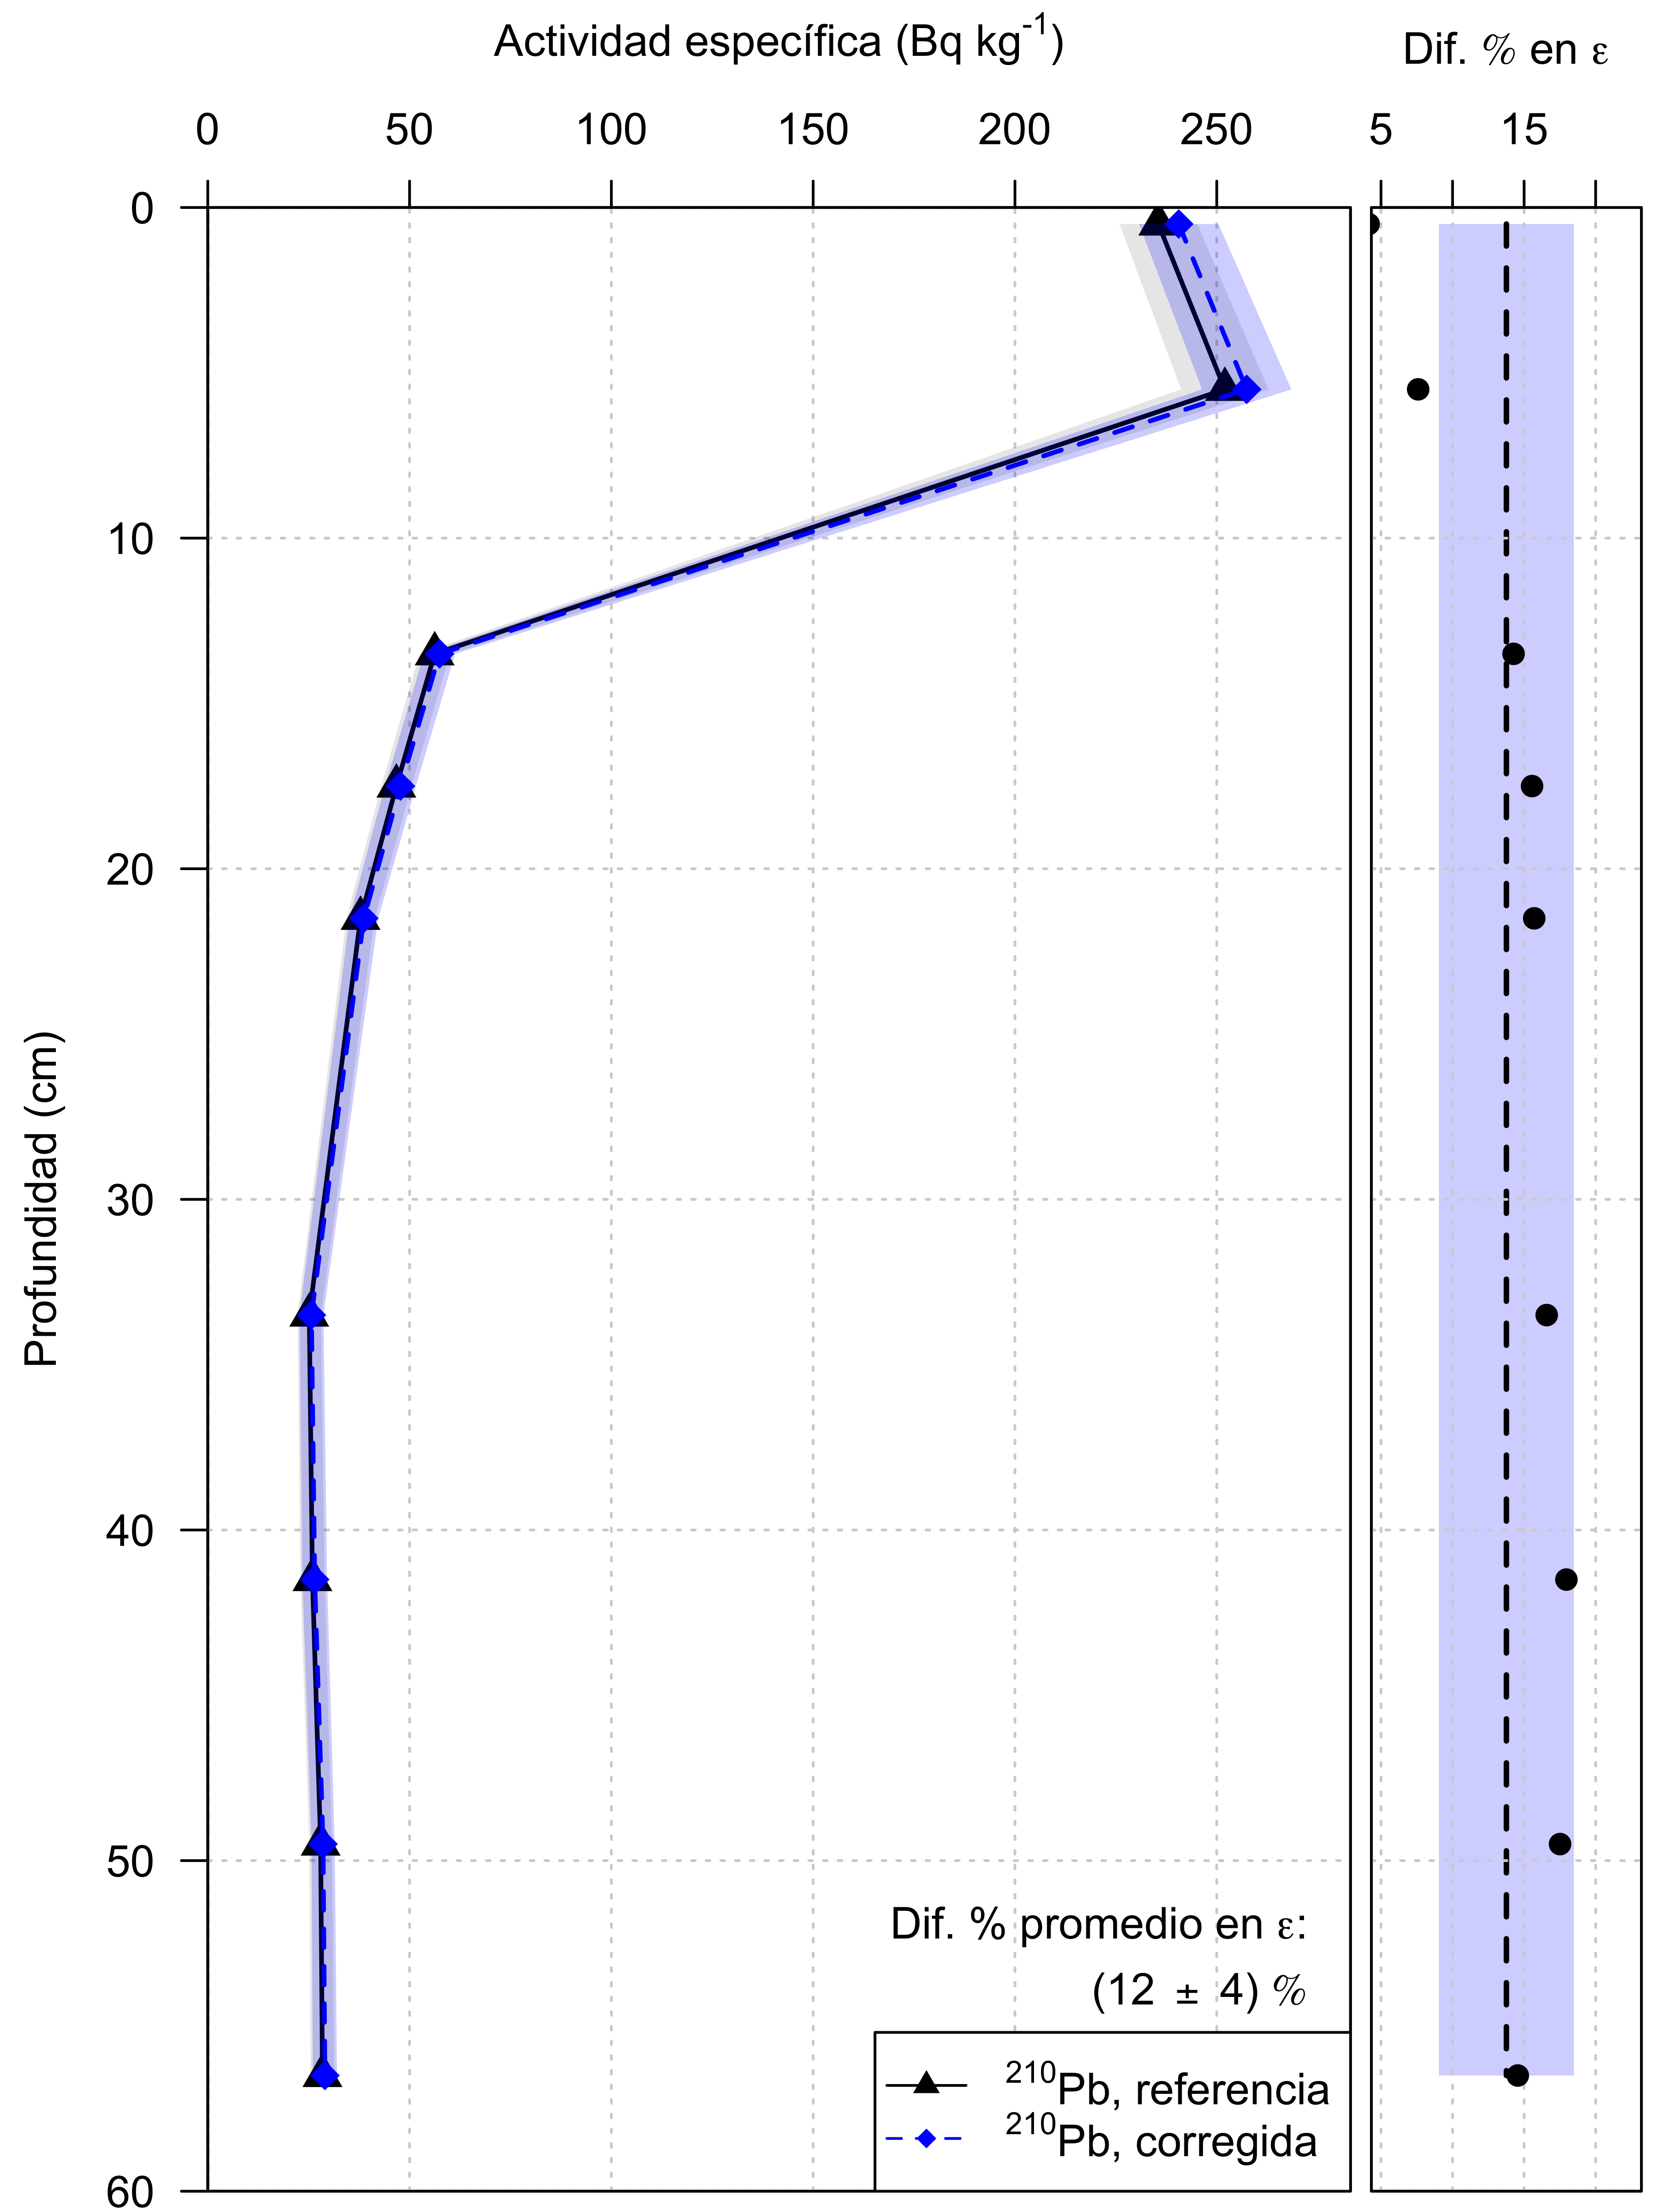
\includegraphics[width=0.9\textwidth]{Imagenes/Act_210Pb_Agua_Composicion_LTAF.png}
\caption{Perfil de actividad específica de \PbCero\, para el núcleo \textbf{LTAF} asumiendo una composición elemental de referencia y una composición corregida (Sección \ref{Secc-100Composicion}). Se muestra la diferencia porcentual promedio en el valor las eficiencias de referencia y corregida para una energía de 46.54 keV.}\label{FigLTAFAgua}
\end{figure}
\begin{figure}
\centering
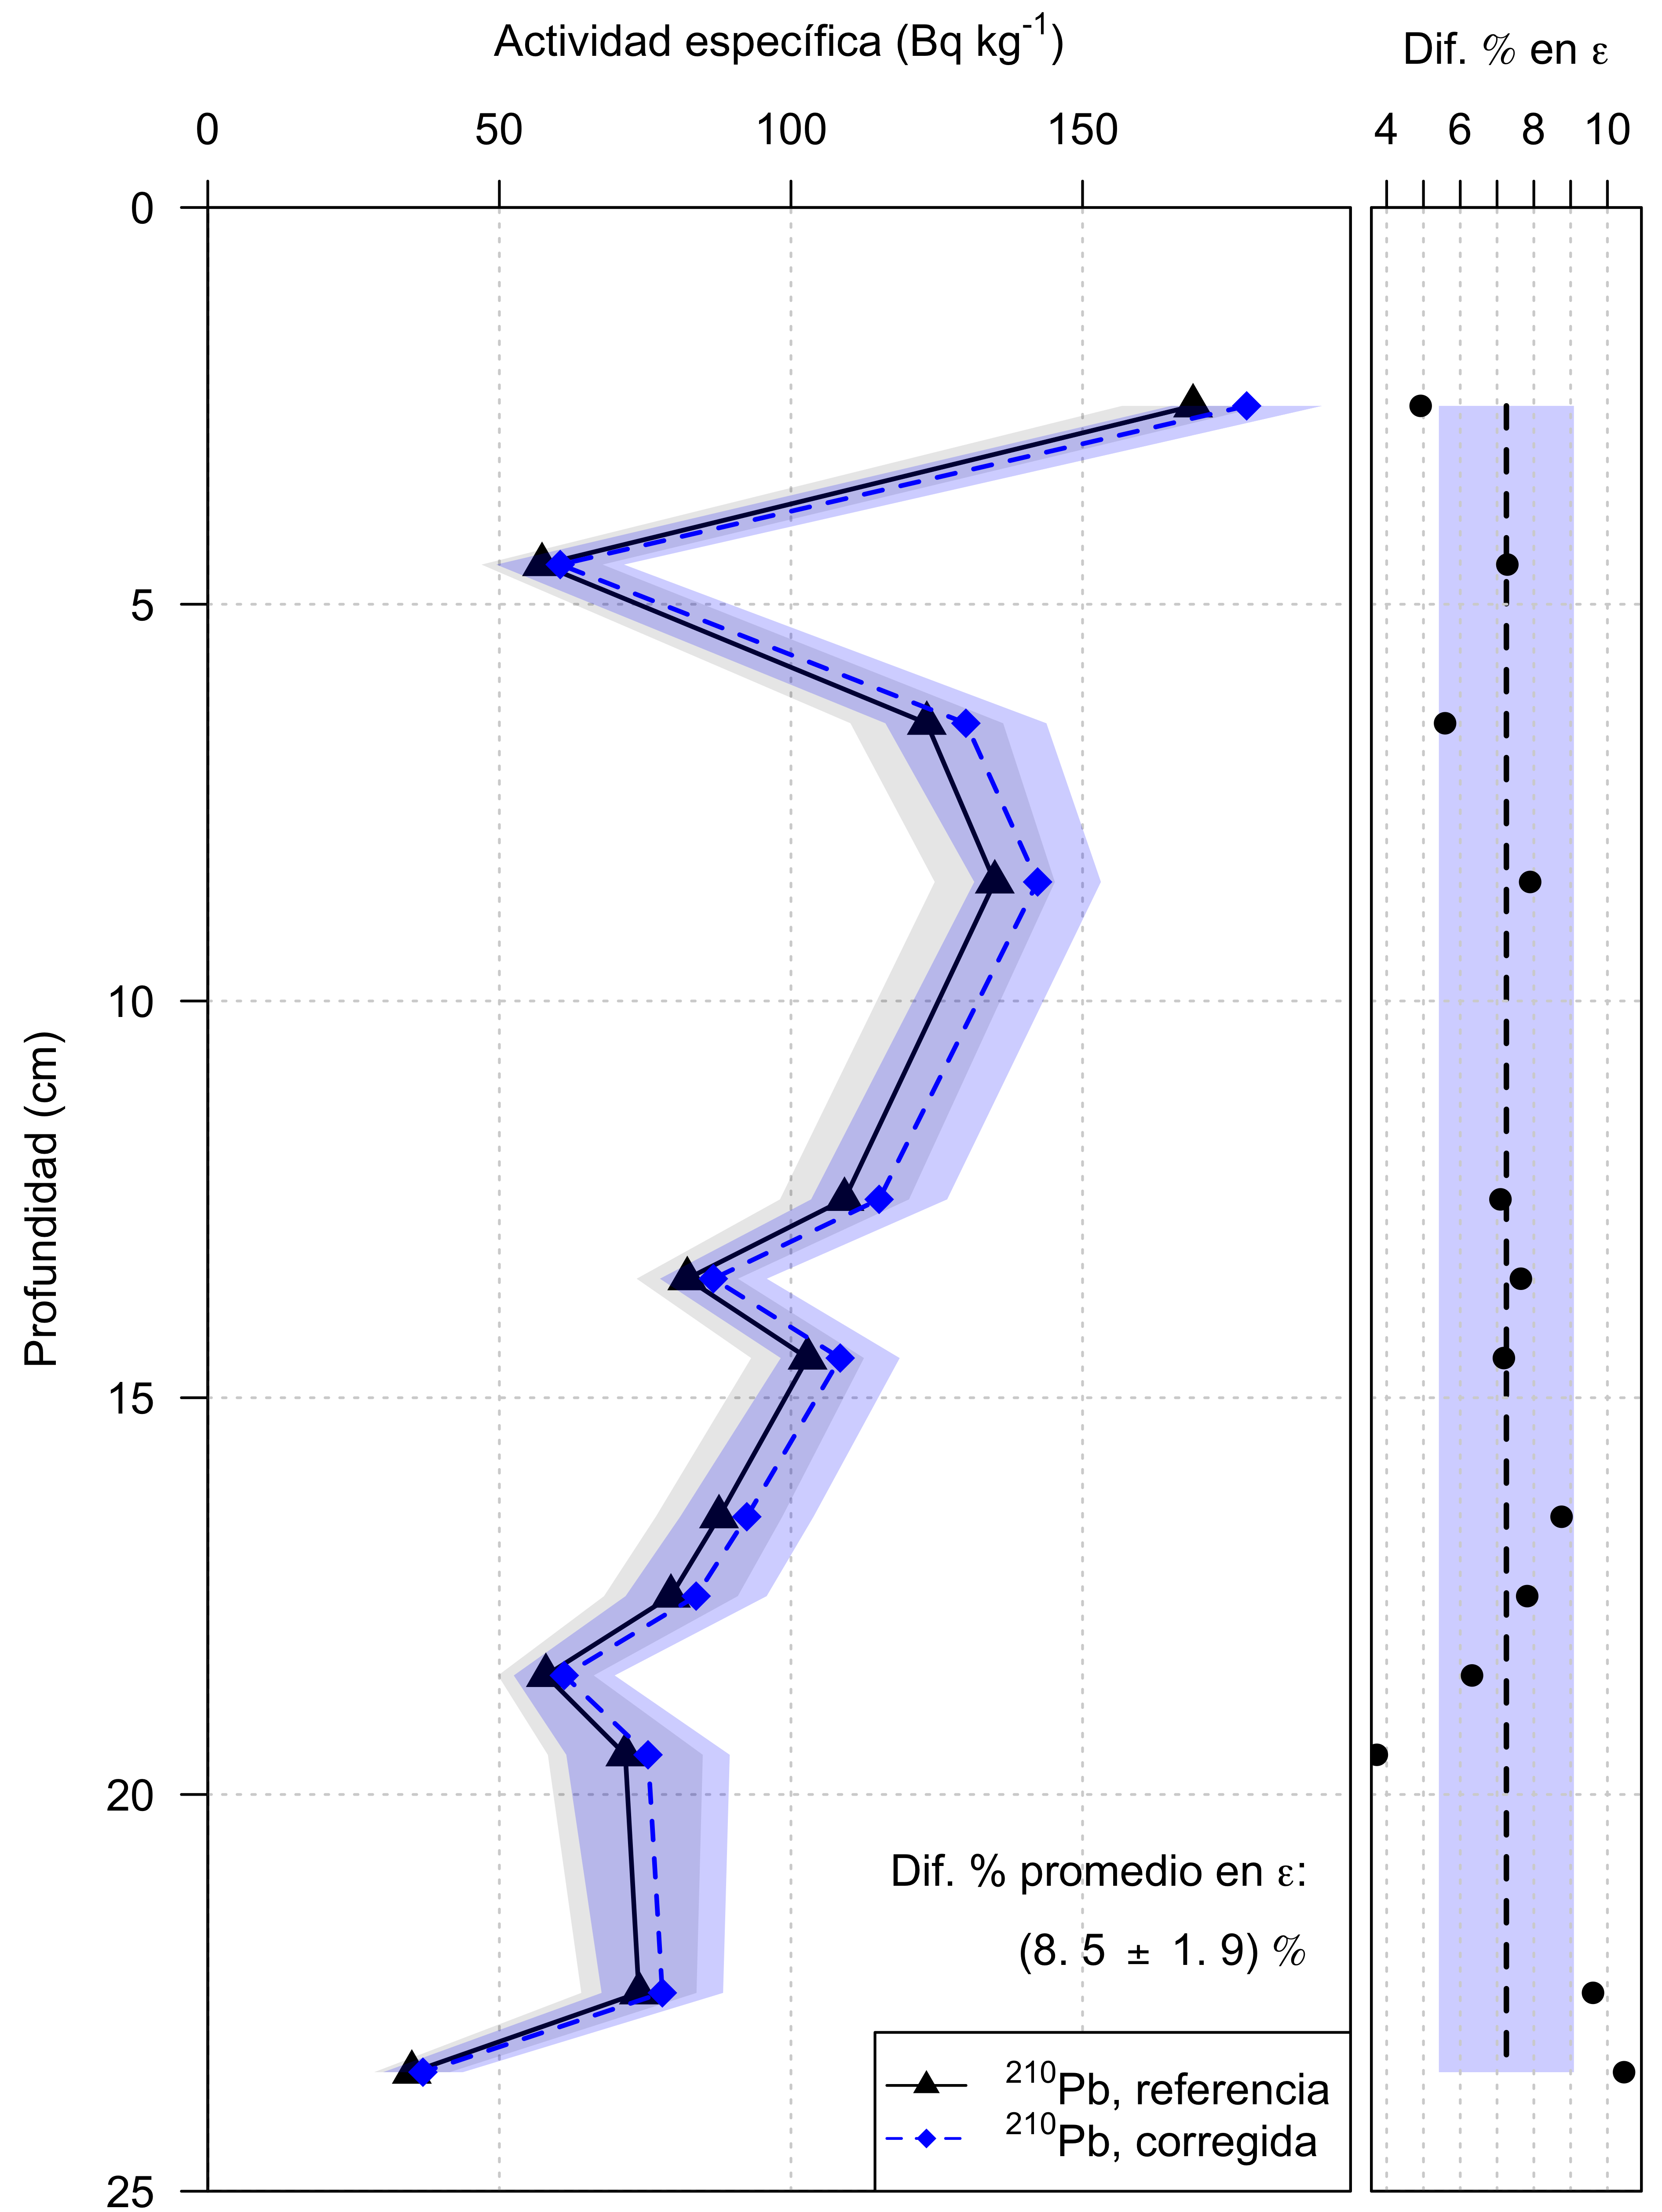
\includegraphics[width=0.9\textwidth]{Imagenes/Act_210Pb_Agua_Composicion_SAMO-14-2.png}
\caption{Perfil de actividad específica de \PbCero\, para el núcleo \textbf{SAMO-14-2} asumiendo una composición elemental de referencia y una composición corregida (Sección \ref{Secc-100Composicion}). Se muestra la diferencia porcentual promedio en el valor las eficiencias de referencia y corregida para una energía de 46.54 keV.}\label{FigSAMO142Agua}
\end{figure}
\begin{figure}
\centering
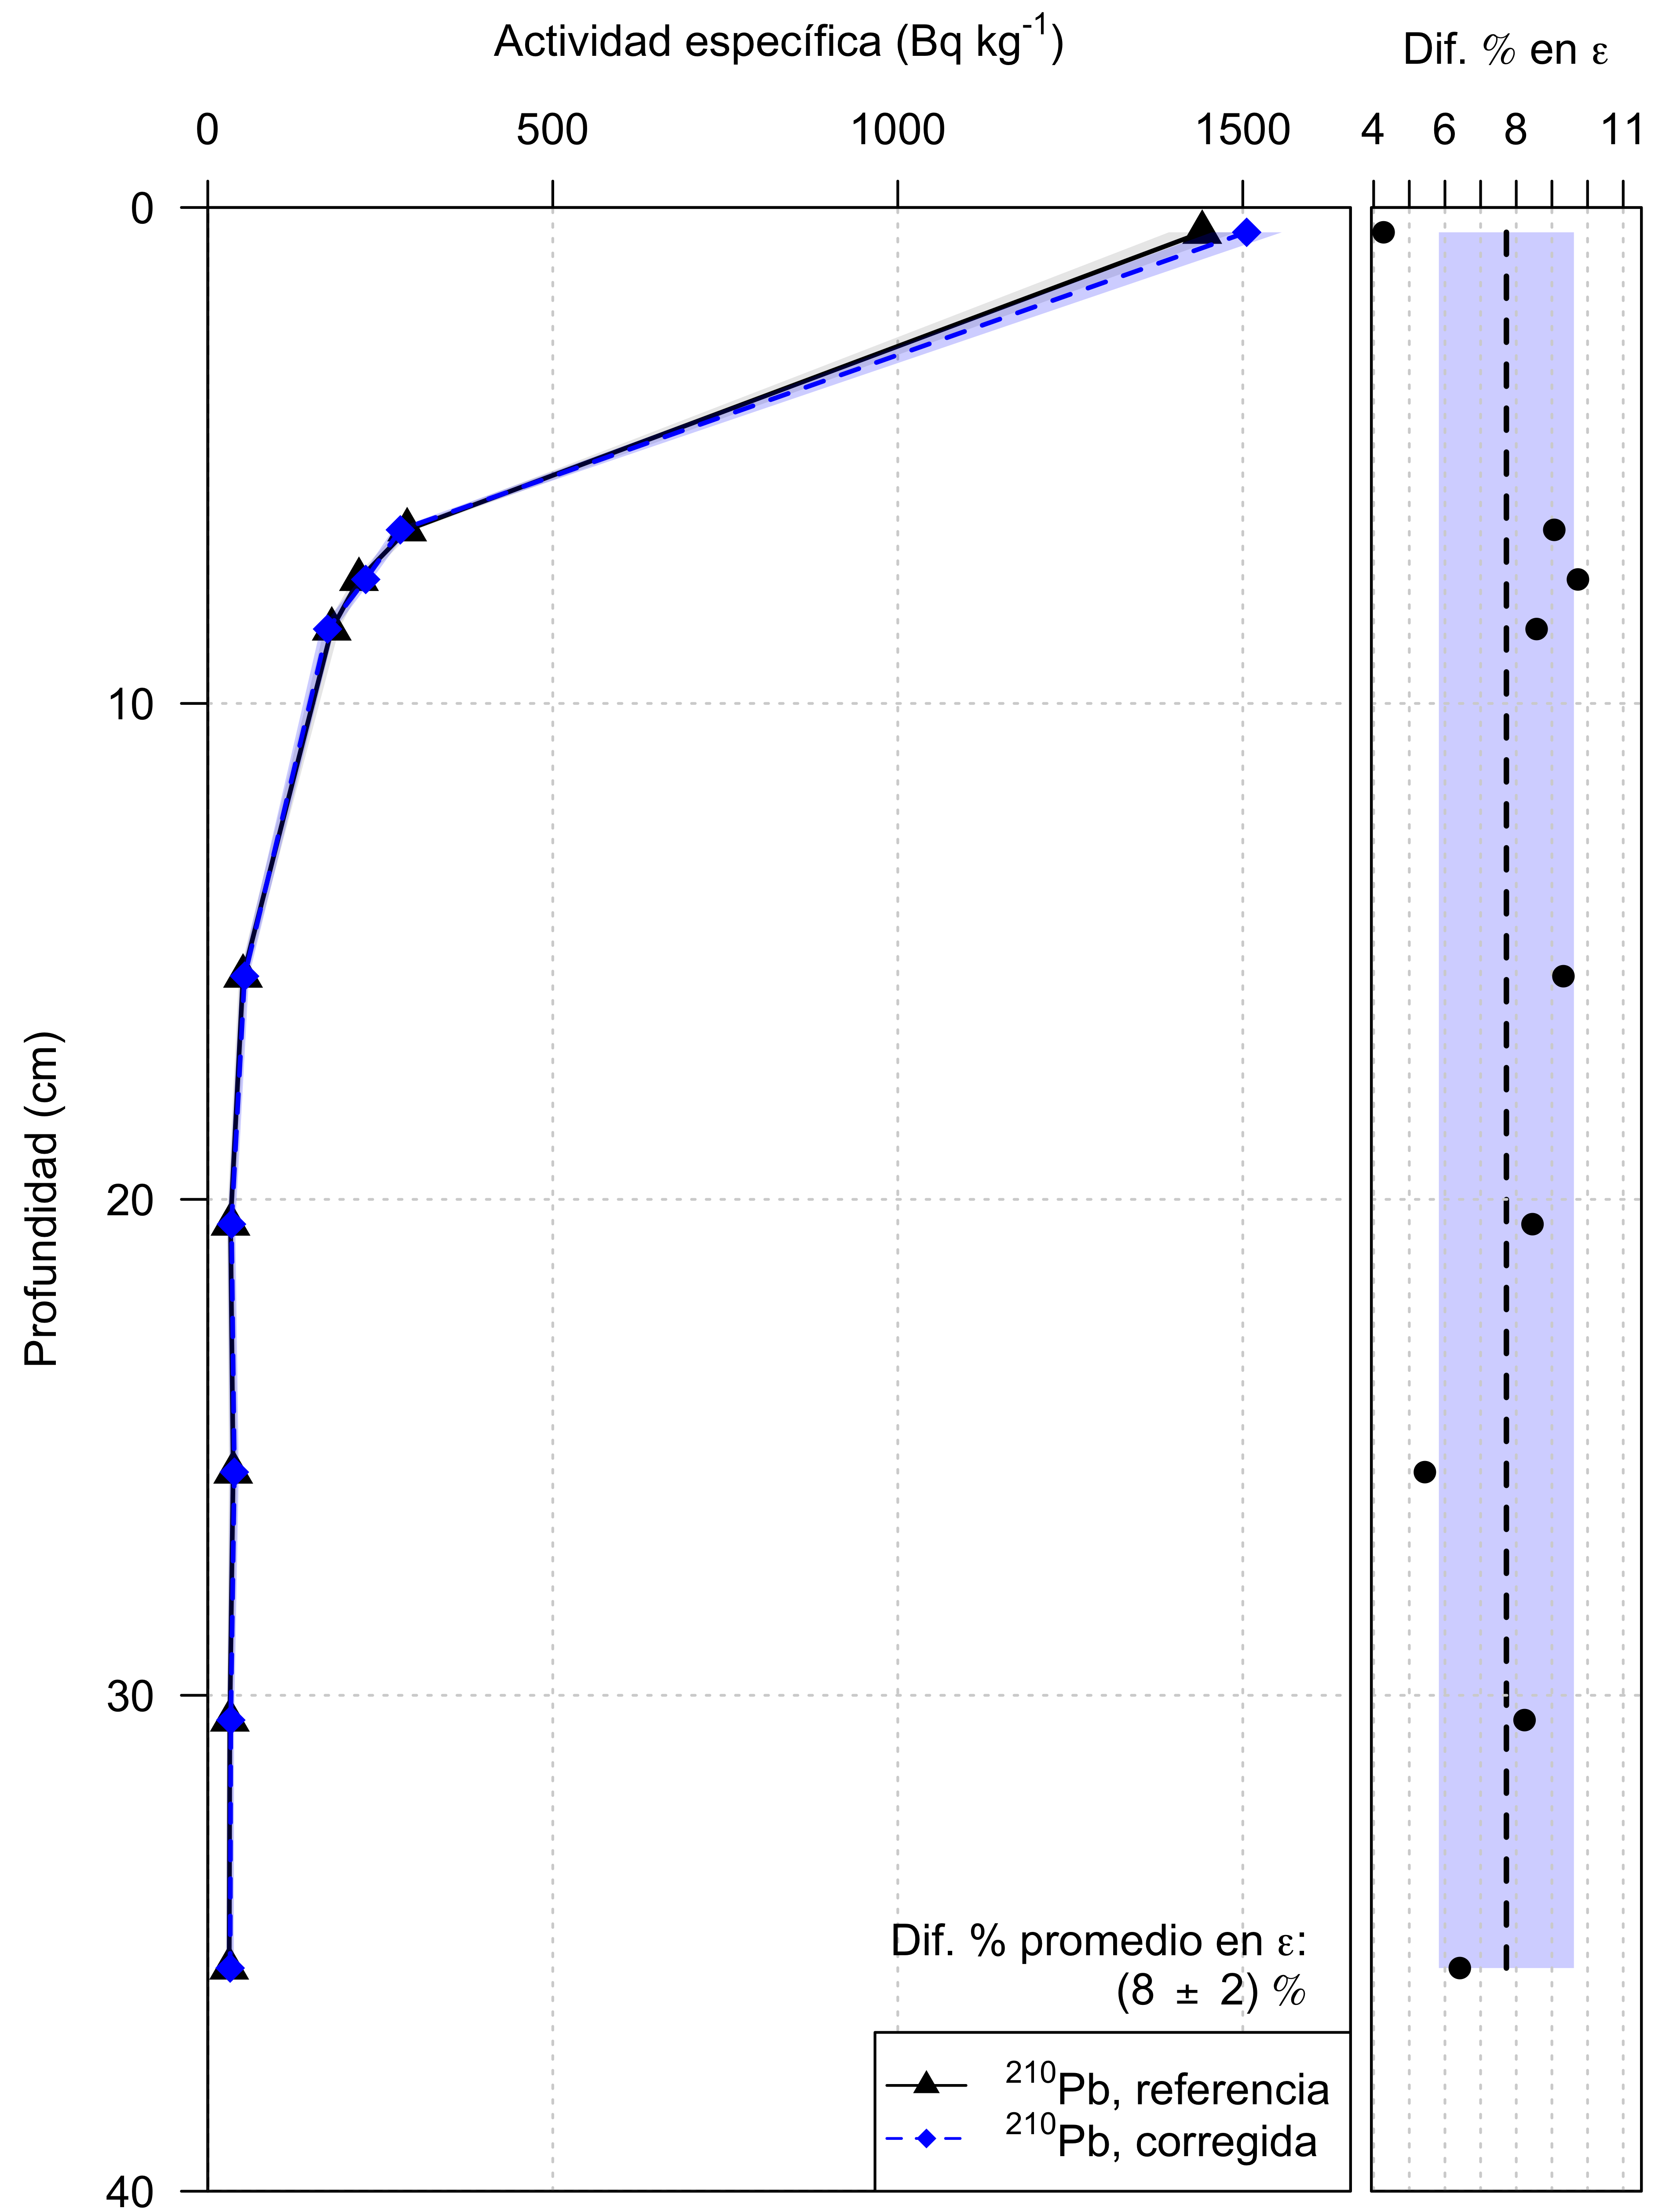
\includegraphics[width=0.9\textwidth]{Imagenes/Act_210Pb_Agua_Composicion_TEHUA-XII.png}
\caption{Perfil de actividad específica de \PbCero\, para el núcleo \textbf{TEHUA-XII} asumiendo una composición elemental de referencia y una composición corregida (Sección \ref{Secc-100Composicion}). Se muestra la diferencia porcentual promedio en el valor las eficiencias de referencia y corregida para una energía de 46.54 keV.}\label{FigTEHUAXIIAgua}
\end{figure}
\newpage
	\section{Equilibrio secular entre \PbCero\, y \PbCuatro}\label{Seccion-210y214}
Debido a la desintegración radiactiva en cadena de \UDosTresOcho\, y al tiempo de vida media de este radionúclido, se espera que los radionúclidos \PbCero\, y \PbCuatro\, se encuentren en equilibrio secular en las secciones más profundas (y por lo tanto más antiguas) de los núcleos sedimentarios. En el fechado con \PbCero\, esta es una información fundamental, pues define el alcance del modelo de fechado. Debido a las altas incertidumbres relativas de las medidas de bajas concentraciones, esta zona es a veces difícil de determinar. Por ejemplo, la última sección del núcleo sedimentario EU-VIII presenta una actividad específica de 2$20.2 \pm 5.8$  Bq kg$^{-1}$, por lo que la  incertidumbre relativa es de un 29 \%. 
\\
\\
En las Figuras \ref{Fig-EUVIII-Comp}, \ref{Fig-GOMRI500-Comp}, \ref{Fig-PCm-Comp}, \ref{Fig-LTAF-Comp}, \ref{Fig-SAMO142-Comp} y \ref{Fig-TEHUAXII-Comp} se muestran los perfiles corregidos de \PbCero\, y \PbCuatro\, y las secciones que posiblemente se encuentran en equilibrio secular. Los rangos de actividad específica y profundidad de los anterior perfiles varían entre núcleos sedimentarios.
\\
\\
De las zonas de manglar, las actividades de las tres últimas secciones medidas en el núcleo sedimentario EU-VIII fueron similares (dentro de las incertidumbres de medida). Sin embargo, en el núcleo PCm, las actividades de \PbCero\, fueron aparentemente superiores a las de \PbCuatro, aunque las incertidumbres se sobreponen y, por lo tanto, podemos considerar que se ha alcanzado el equilibrio secular. 
\\
\\
Un comportamiento inverso fue observado en el núcleo LTAF, pues las actividades de \PbCero\, son en este caso inferiores al \PbCuatro, lo que significa la presencia de un déficit de \PbCero, probablemente  debido a un enriquecimiento de \Ra\, (en equilibrio con el \PbCuatro) debido a procesos diagenéticos. De hecho, LTAF es el núcleo sedimentario de manglar con mayor concentración de \PbCero, que puede ser debido a la migración hacia la superficie de \Ra<  \, de capas inferiores, causando así su exceso respecto al \PbCero. Esto es consistente con el decrecimiento del \PbCuatro\, en las capas superficiales, indicando que parte del \Ra\, está siendo transferido al agua intersticial, y de aquí a la columna de agua. En estos casos, es recomendable utilizar las concentraciones de \PbCero\, en el fondo del núcleo para estimar un valor constante del \PbCeroEx. 
\\
\\
En este caso, se asigna que las 4 últimas secciones medidas del núcleo LTAF pertenecen a la zona de equilibrio secular con un valor promedio de las actividades específicas de \PbCero\, de $31.6 \pm 9.9$ Bq kg$^{-1}$ (coeficiente de variación del 31 \%) y un valor promedio de las actividades específicas de \PbCuatro\, de $40.0 \pm 12.1$ Bq kg$^{-1}$ (coeficiente de variación del 30 \%). Utilizando el test estadístico $Z$ (o método $Z$-score), inferimos que estas distribuciones no son diferentes ($p$ < 0.05). 
\\
\\
Los núcleos de mar abierto fueron los que mostraron una mayor corrección de eficiencia. En el núcleo sedimentario GOMRI-500 las concentraciones de \PbCero\, fueron algo superiores que las de \PbCuatro, pero dentro de las incertidumbres en dos de las tres secciones. Contrariamente, las concentraciones de \PbCero\, fueron algo inferiores a las de \PbCuatro\, en el núcleo TEHUA-XII, si bien todas las secciones mostraron equilibrio secular dentro de las incertidumbres. Por lo tanto concluimos que en ambos casos se llegó al equilibrio secular. En el caso del núcleo sedimentario GOMRI-500 se observó una zona de equilibrio en la mitad del núcleo, que muy probablemente indica el registro de un evento natural o antropogénico, cuya discusión está fuera del alcance de este trabajo. Para el núcleo lacustre SAMO-14-2, tan sólo una de las secciones medidas está en la zona de equilibrio, si bien las concentraciones son prácticamente idénticas, por lo que concluimos que se llegó a la zona de equilibrio secular. 
\\
\\
Para cuantificar estas observaciones empíricas, se definió la variable $\delta$ (ver Figura \ref{Fig-DiffPorcentualEquilibrio}) como la diferencia porcentual  de  la  actividad  específica  de  \PbCero\, respecto a la actividad específica de \PbCuatro\, para las secciones que se encuentran en la zona de equilibrio secular, 
\begin{equation}
\delta = \dfrac{A(^{214}\text{Pb}) - A(^{210}\text{Pb}) }{A(^{214}\text{Pb}) } \times 100.
\end{equation}
En el Apéndice \ref{ApexZonaEquilibrio} se muestran las secciones de los núcleos sedimentarios en donde se asume equilibrio secular, aquellas en donde las actividades corregidas de \PbCero\, y \PbCuatro\, se superponen al incluir las incertidumbres. Utilizando las secciones pertenecientes a la zona de equilibrio (37.5 cm, 45.5 cm y 53.5 cm del núcleo EU-VIII, 12.25 cm y 21.75 cm del núcleo GOMRI-500 y la sección 23.5 cm del SAMO-14-2), se obtuvo un valor promedio de $\overline{\delta} = 7 \pm 8$, que incluye al cero y confirma que los criterios utilizados para detectar la presencia de equilibrio secular son correctas. Cabe resaltar que las desviaciones $\delta$ para algunas secciones pertenecientes a la zona de equilibrio son en algunos casos altas y que éstas pueden ser debidas a razones geoquímicas y no de calibración de los sistemas de espectrometría de rayos gamma. 
\begin{figure}
\centering
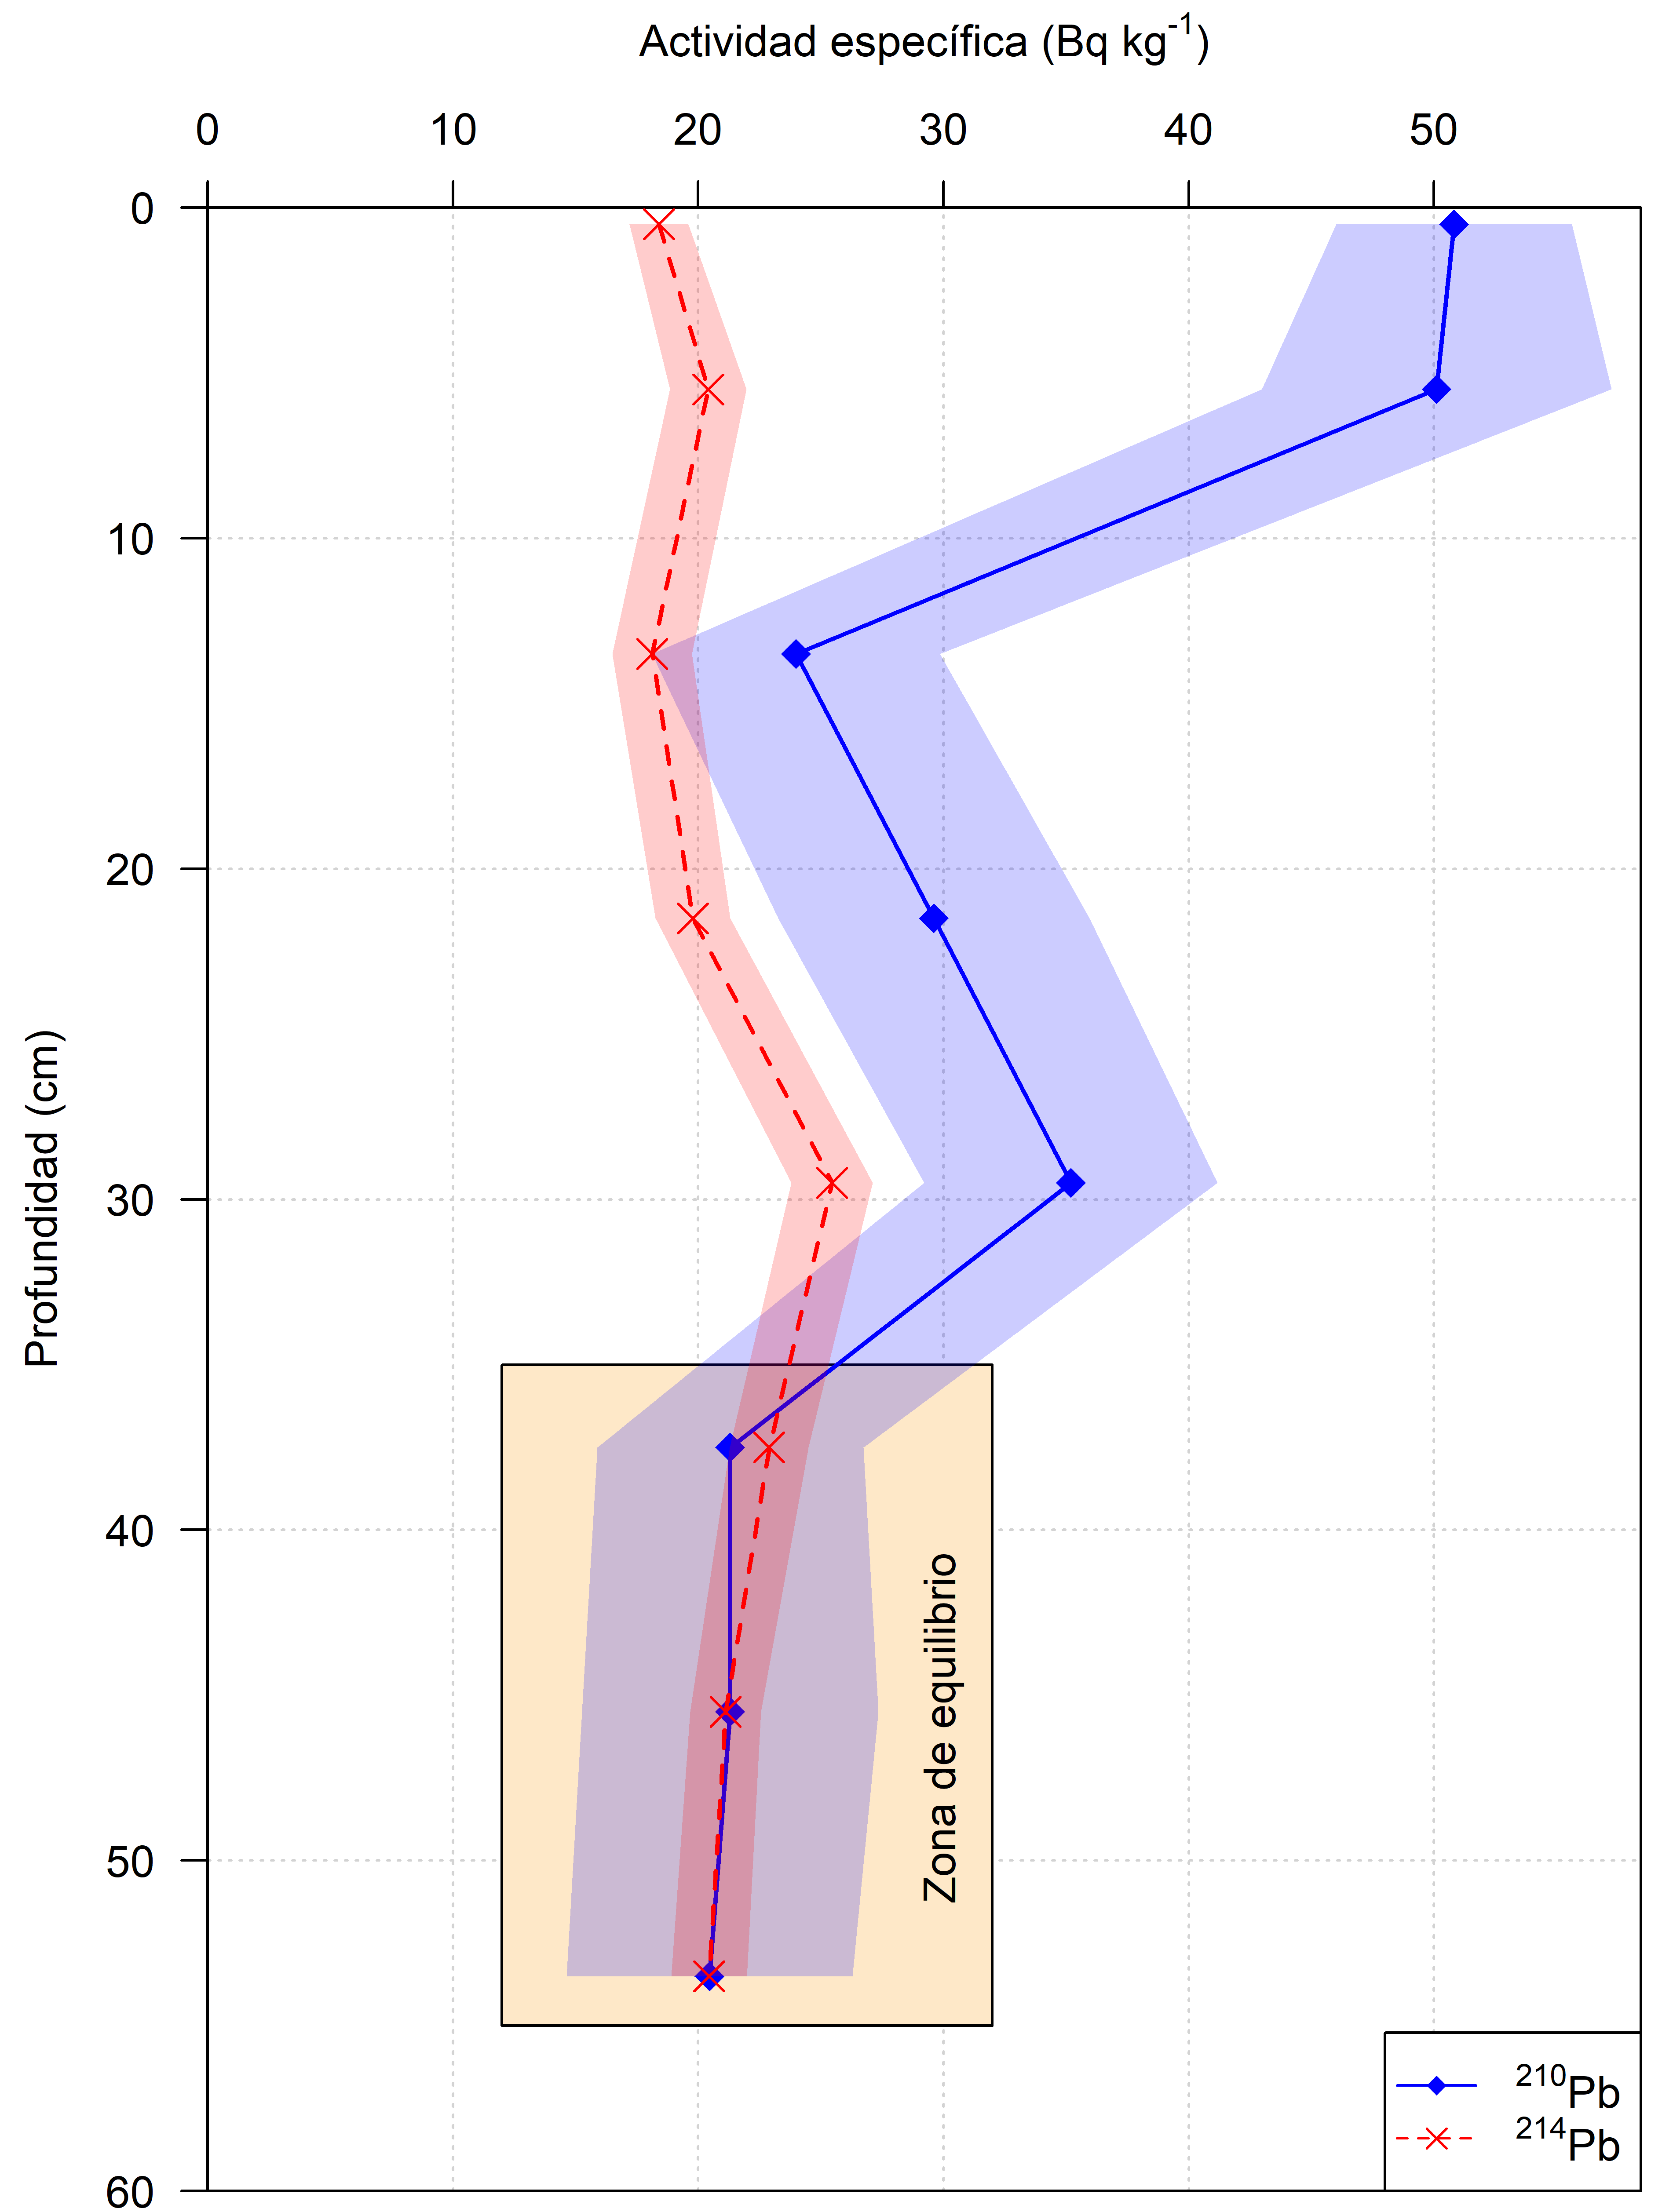
\includegraphics[width=0.9\textwidth]{Imagenes/Act_210Pb_214Pb_EU_VIII.png}
\caption{Perfiles de actividad específica de \PbCero\, y \PbCuatro\,corregidos para el núcleo sedimentario \textbf{EU-VIII}. Las tres últimas secciones posiblemente se encuentran en equilibrio secular.}\label{Fig-EUVIII-Comp}
\end{figure}
\begin{figure}
\centering
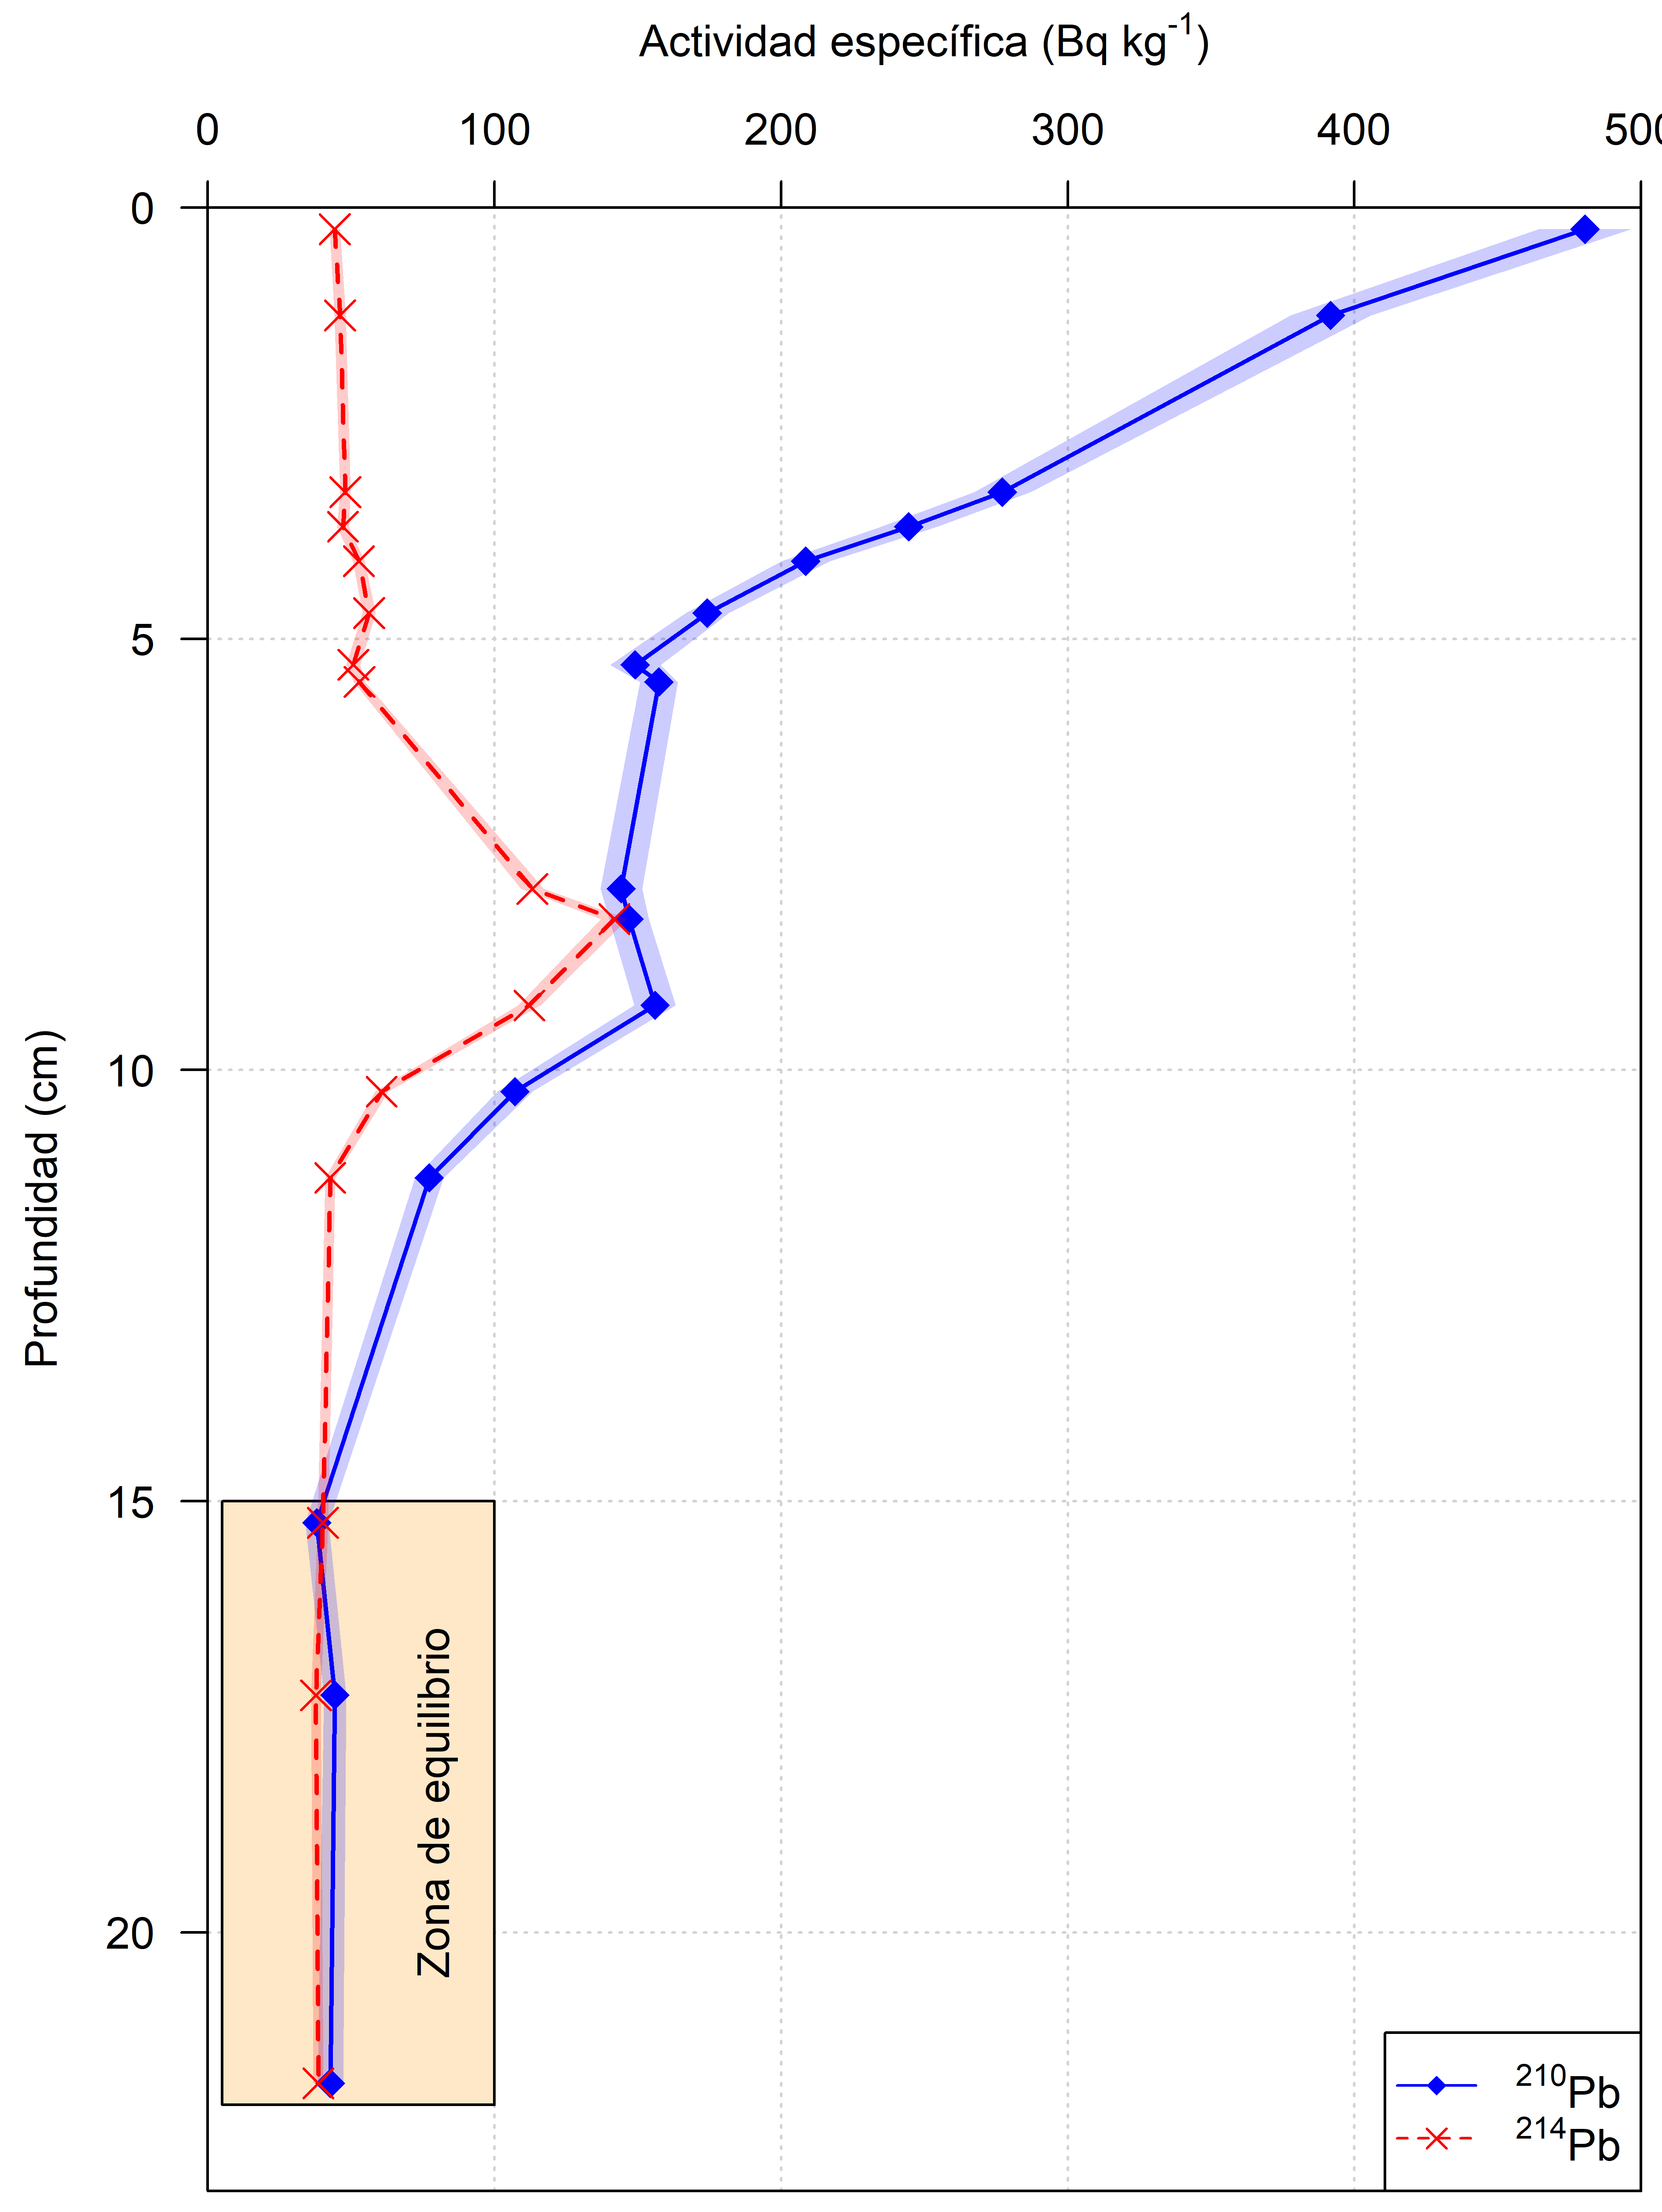
\includegraphics[width=0.9\textwidth]{Imagenes/Act_210Pb_214Pb_GOMRI_500.png}
\caption{Perfiles de actividad específica de \PbCero\, y \PbCuatro\, corregidos para el núcleo sedimentario \textbf{GOMRI-500}. Las tres últimas secciones posiblemente se encuentran en equilibrio secular.}\label{Fig-GOMRI500-Comp}
\end{figure}
\begin{figure}
\centering
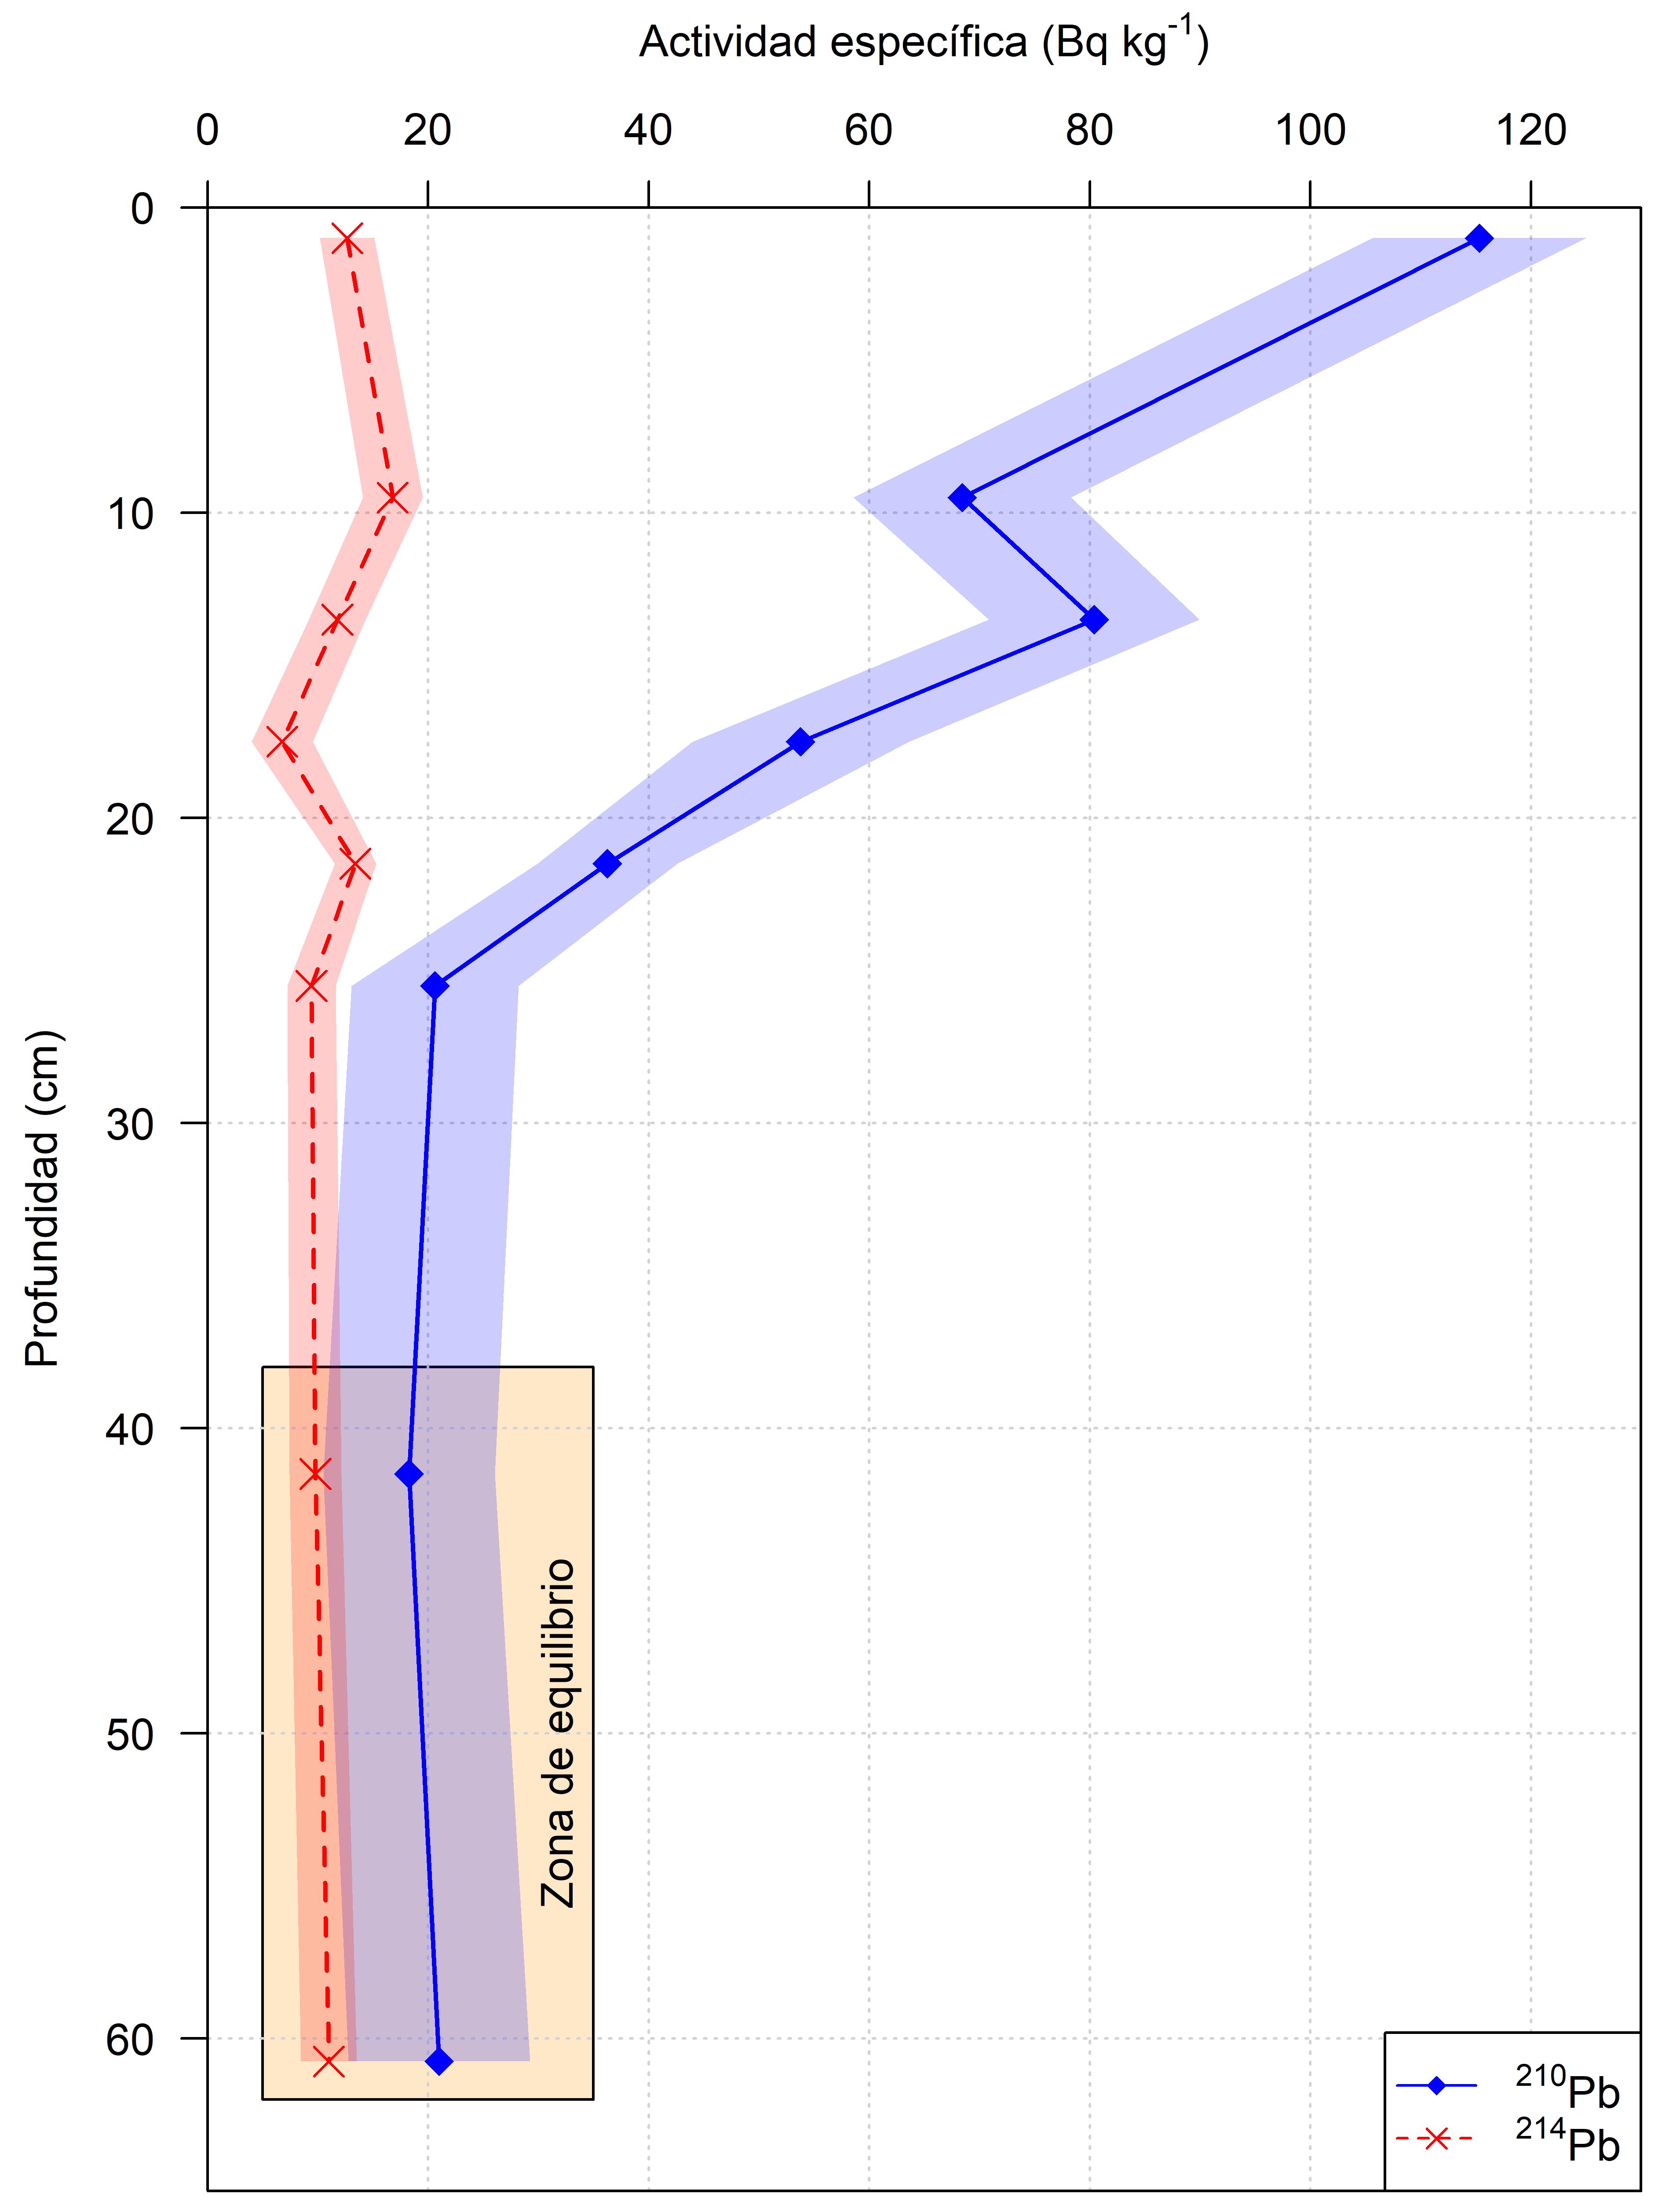
\includegraphics[width=0.9\textwidth]{Imagenes/Act_210Pb_214Pb_PCm.png}
\caption{Perfiles de actividad específica de \PbCero\, y \PbCuatro\,corregidos para el núcleo sedimentario \textbf{PCm}. Las dos últimas secciones posiblemente se encuentran en equilibrio secular.}\label{Fig-PCm-Comp}
\end{figure}
\begin{figure}
\centering
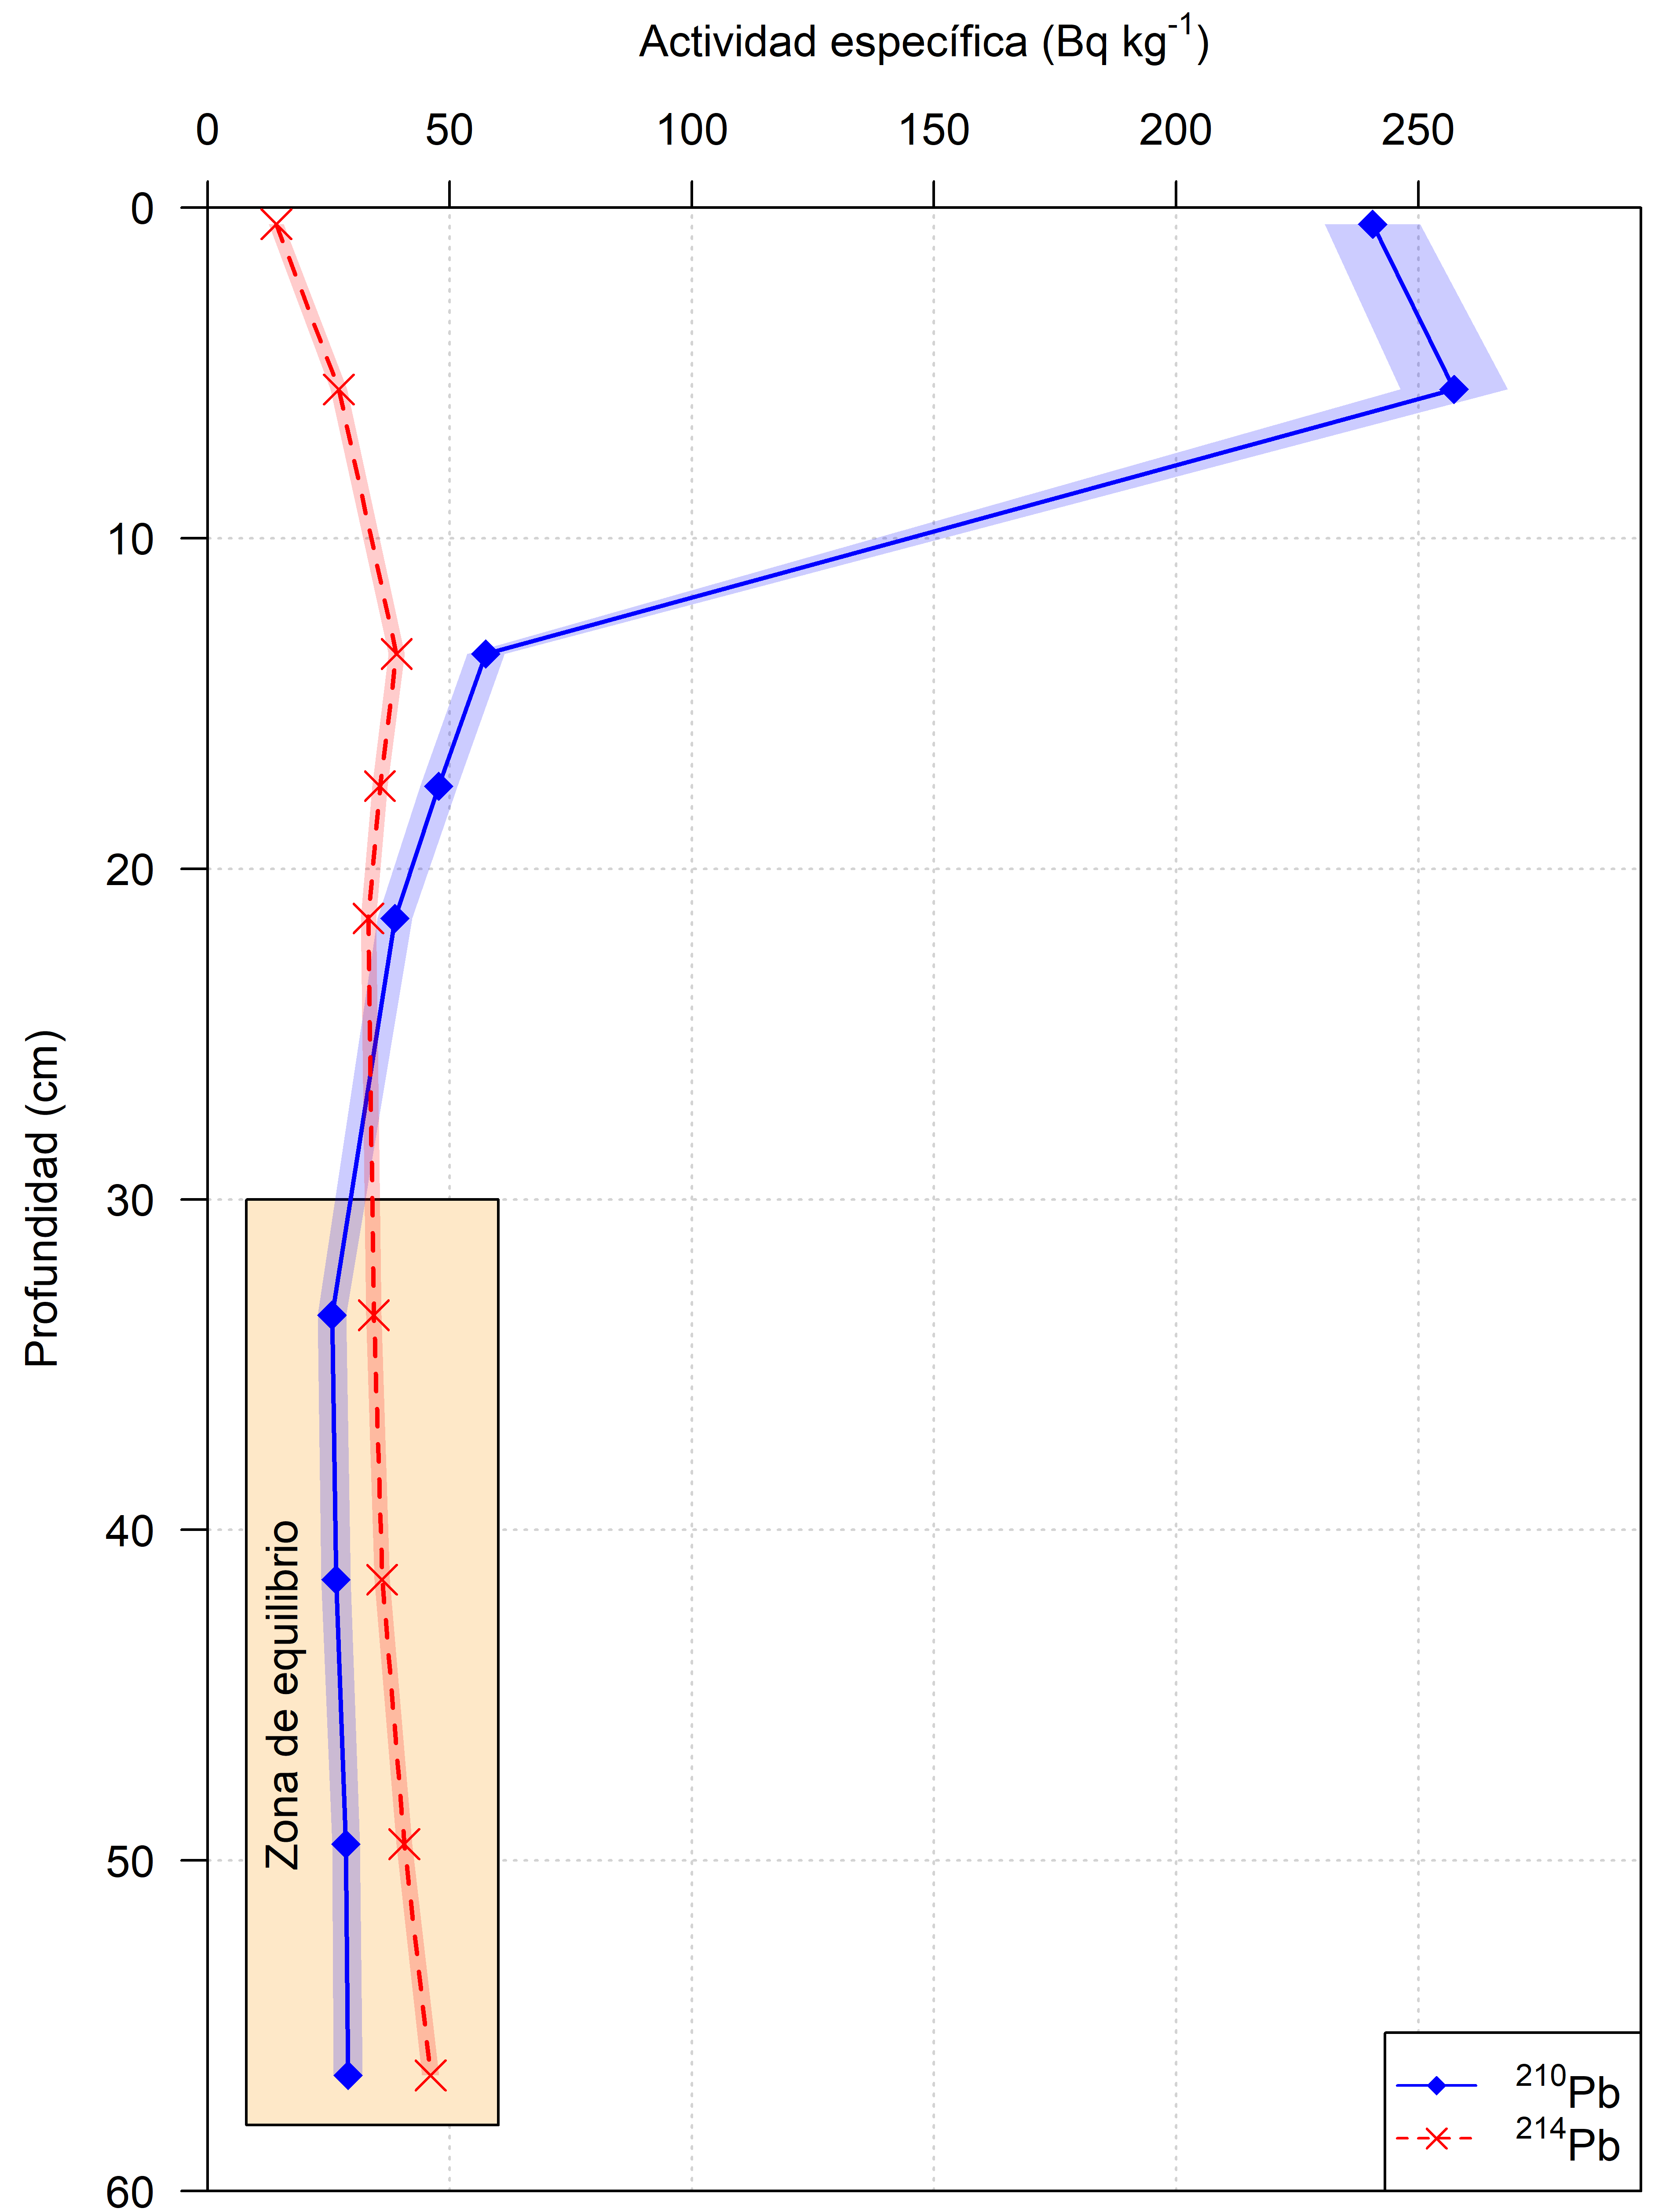
\includegraphics[width=0.9\textwidth]{Imagenes/Act_210Pb_214Pb_LTAF.png}
\caption{Perfiles de actividad específica de \PbCero\, y \PbCuatro\,corregidos para el núcleo sedimentario \textbf{LTAF}. Las tres últimas secciones posiblemente se encuentran en equilibrio secular.}\label{Fig-LTAF-Comp}
\end{figure}
\begin{figure}
\centering
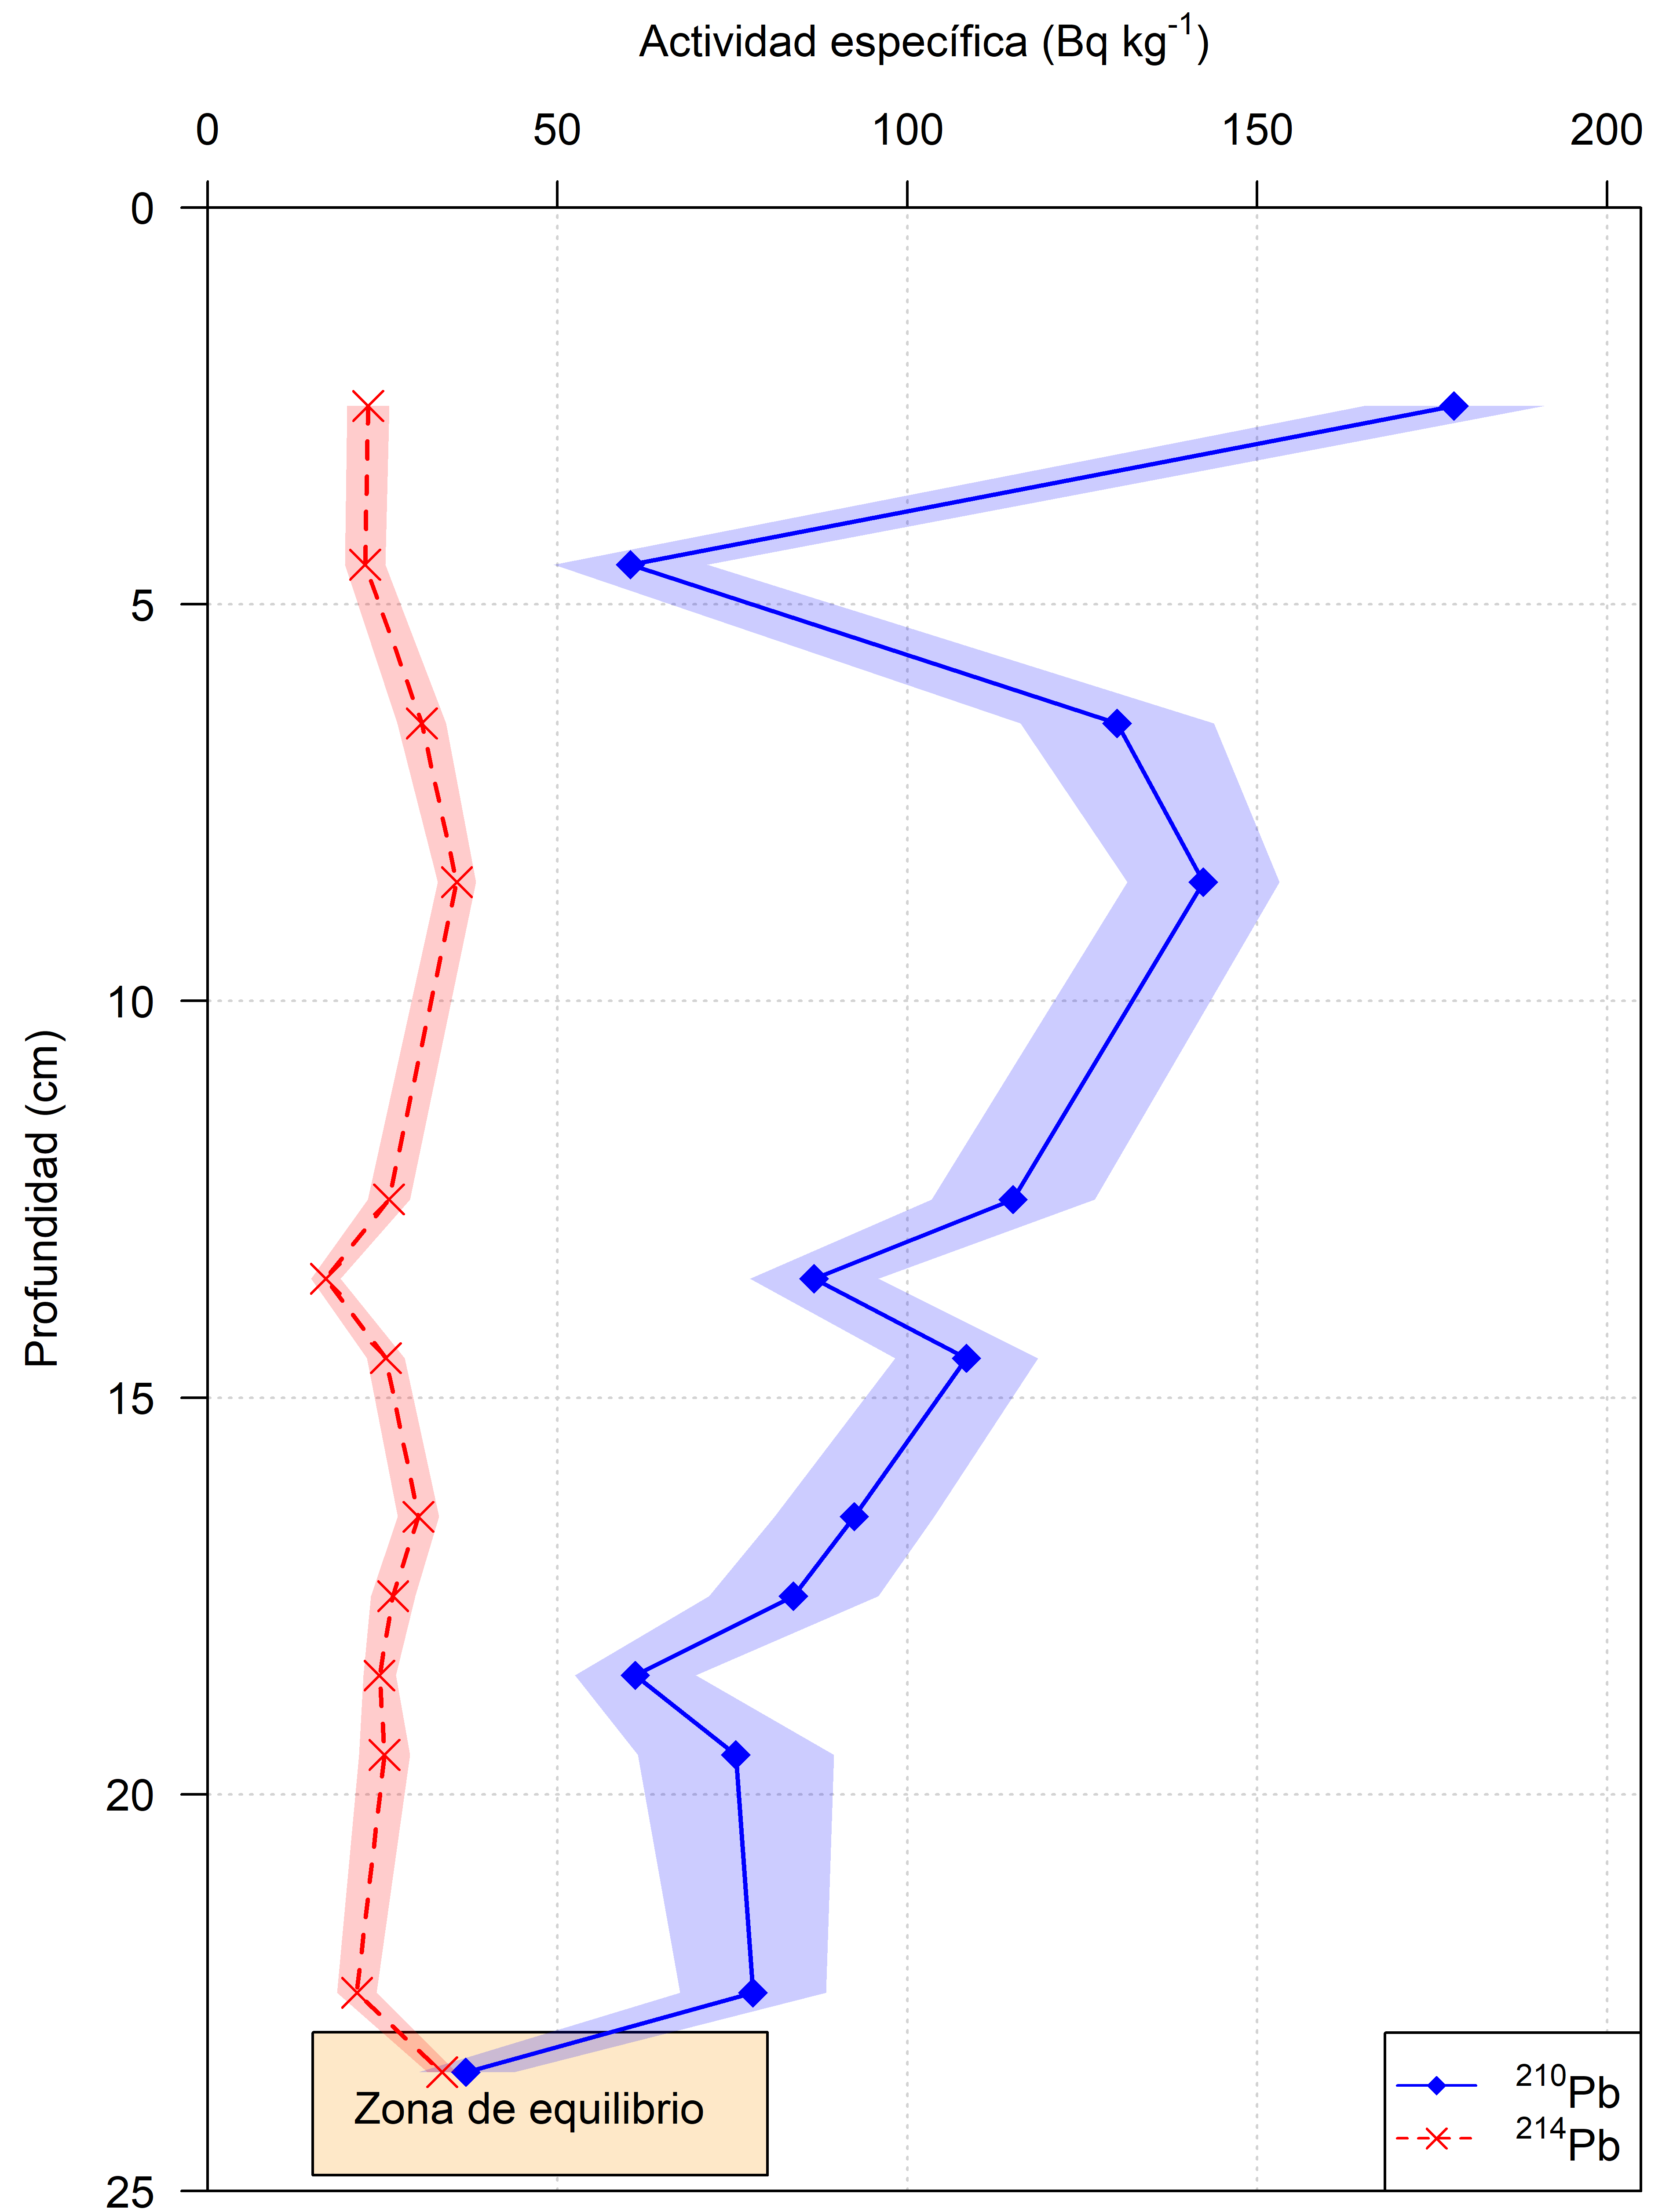
\includegraphics[width=0.9\textwidth]{Imagenes/Act_210Pb_214Pb_SAMO-14-2.png}
\caption{Perfiles de actividad específica de \PbCero\, y \PbCuatro\,corregidos para el núcleo sedimentario \textbf{SAMO-14-2}. La última sección posiblemente se encuentra en equilibrio secular.}\label{Fig-SAMO142-Comp}
\end{figure}
\begin{figure}
\centering
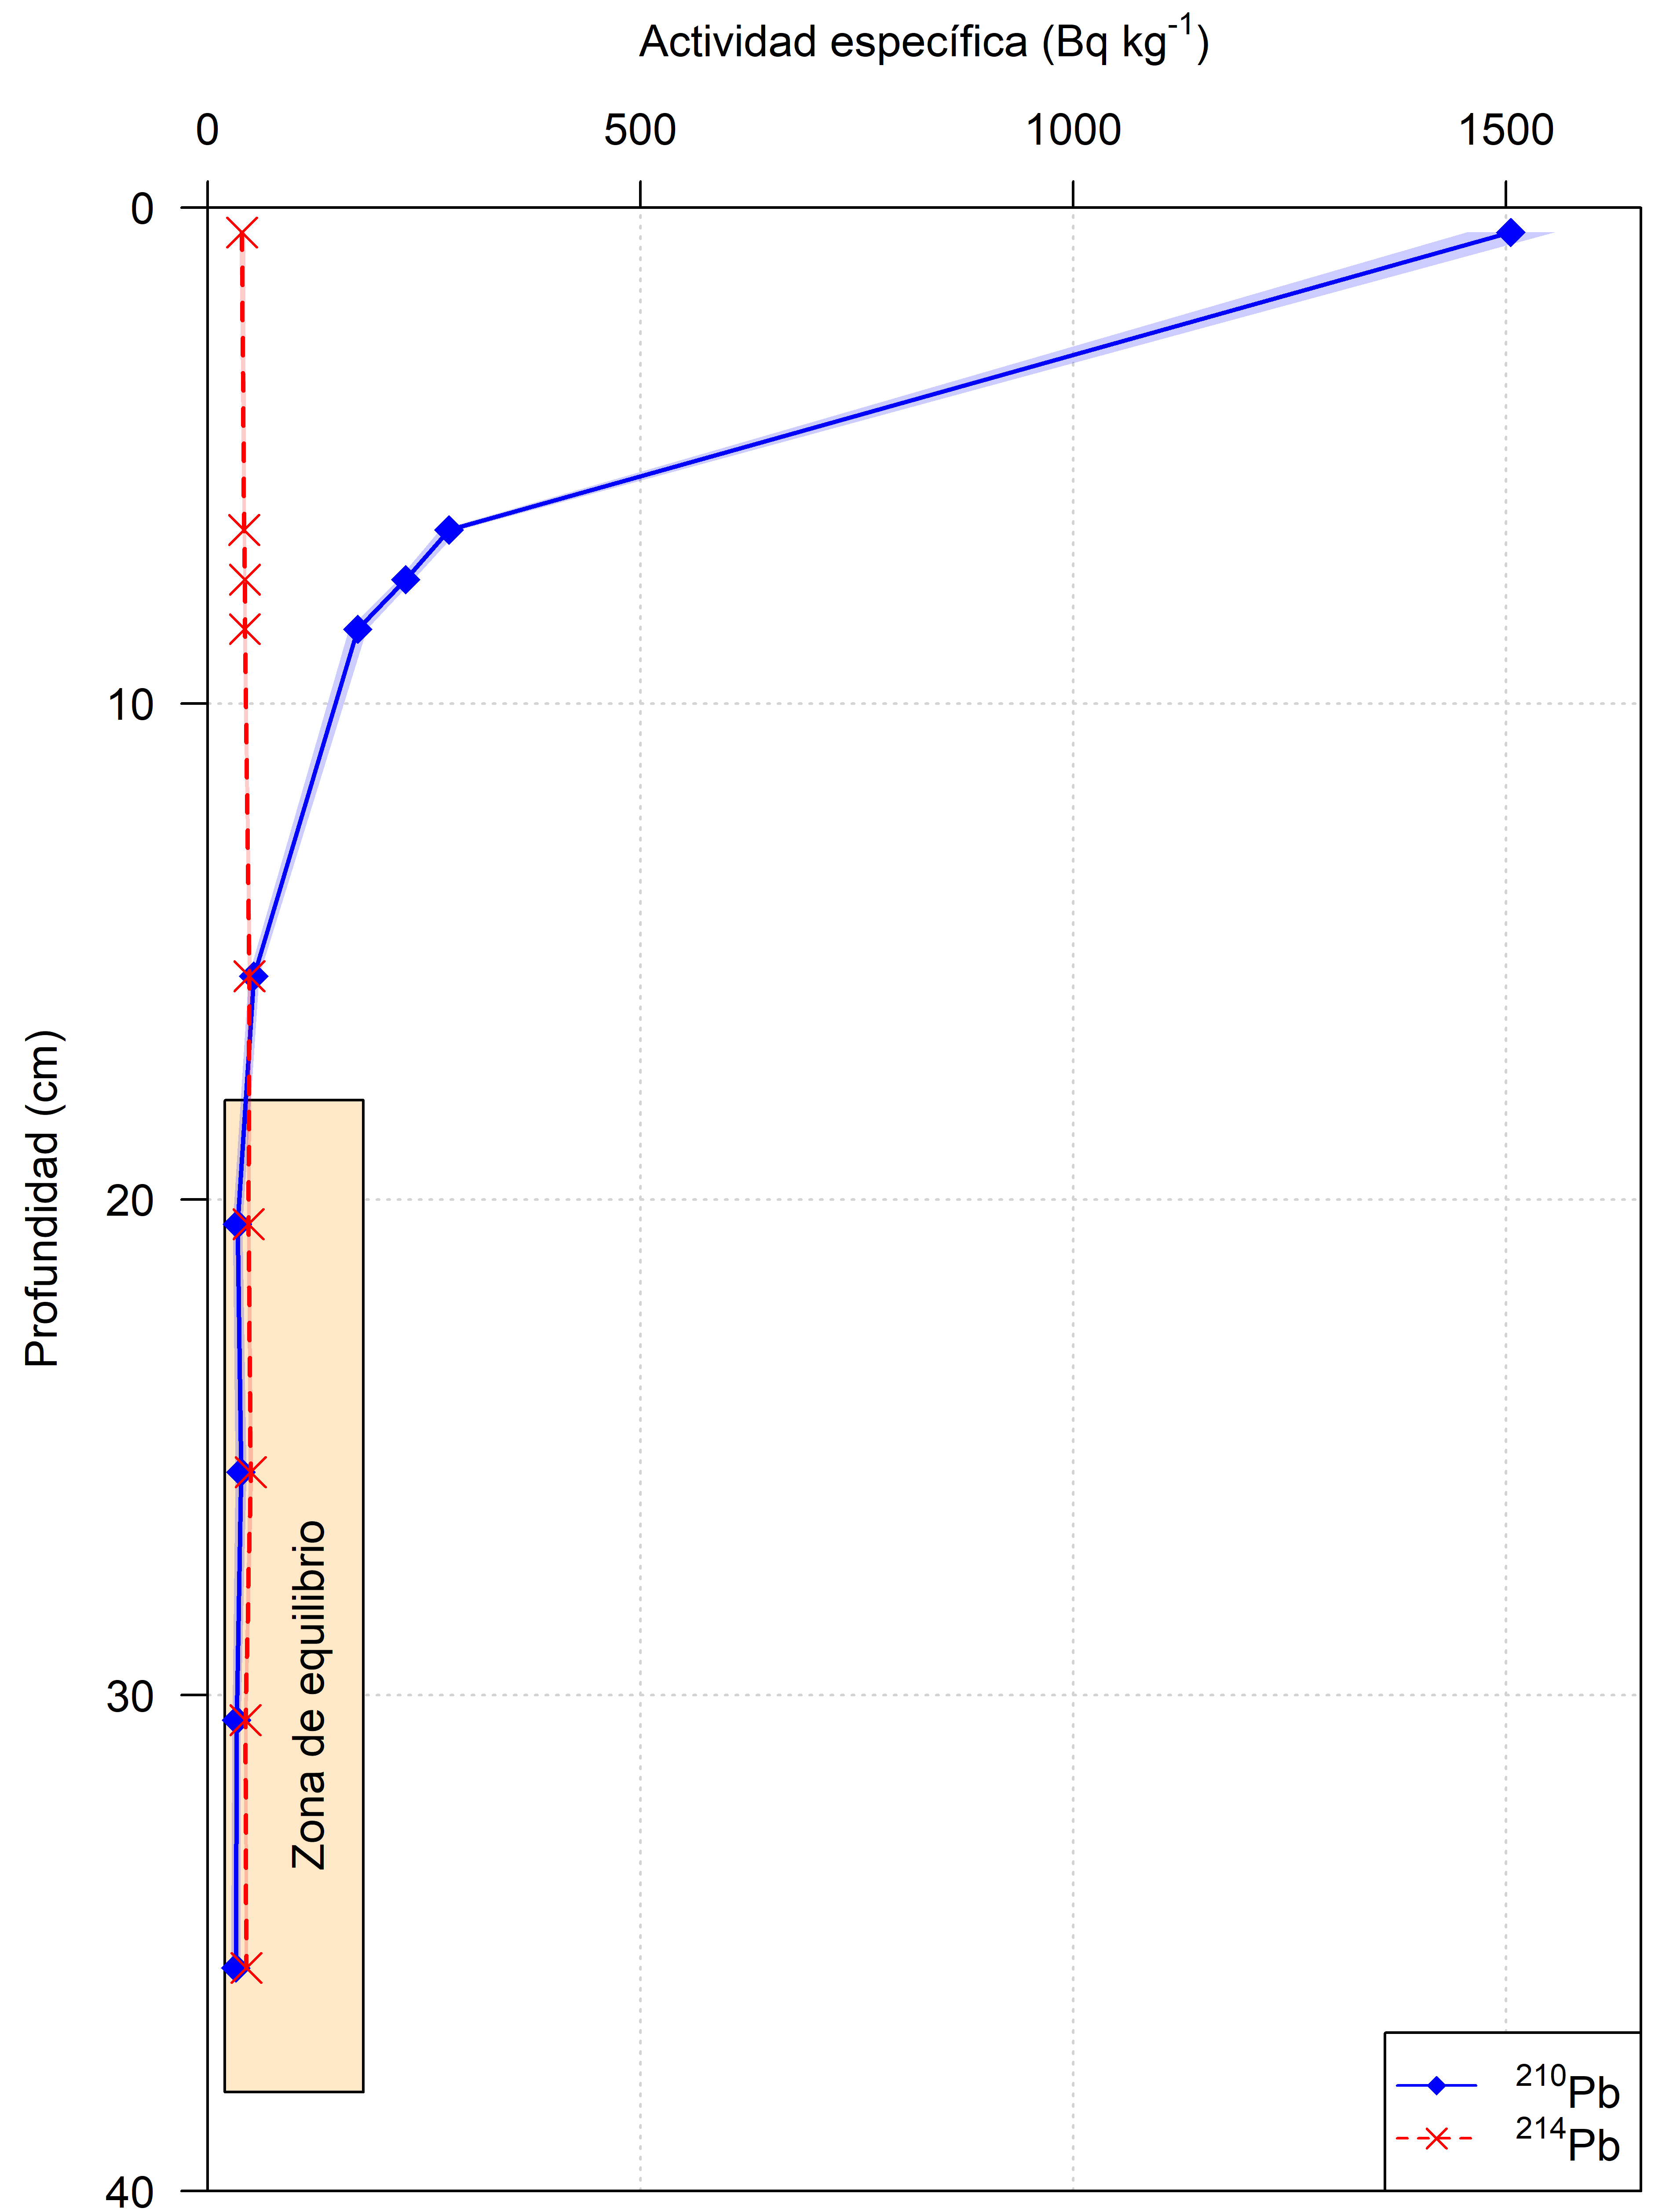
\includegraphics[width=0.9\textwidth]{Imagenes/Act_210Pb_214Pb_TEHUA-XII.png}
\caption{Perfiles de actividad específica de \PbCero\, y \PbCuatro\,corregidos para el núcleo sedimentario \textbf{TEHUA-XII}. Las cuatro últimas secciones posiblemente se encuentran en equilibrio secular.}\label{Fig-TEHUAXII-Comp}
\end{figure}
\begin{figure}
\centering
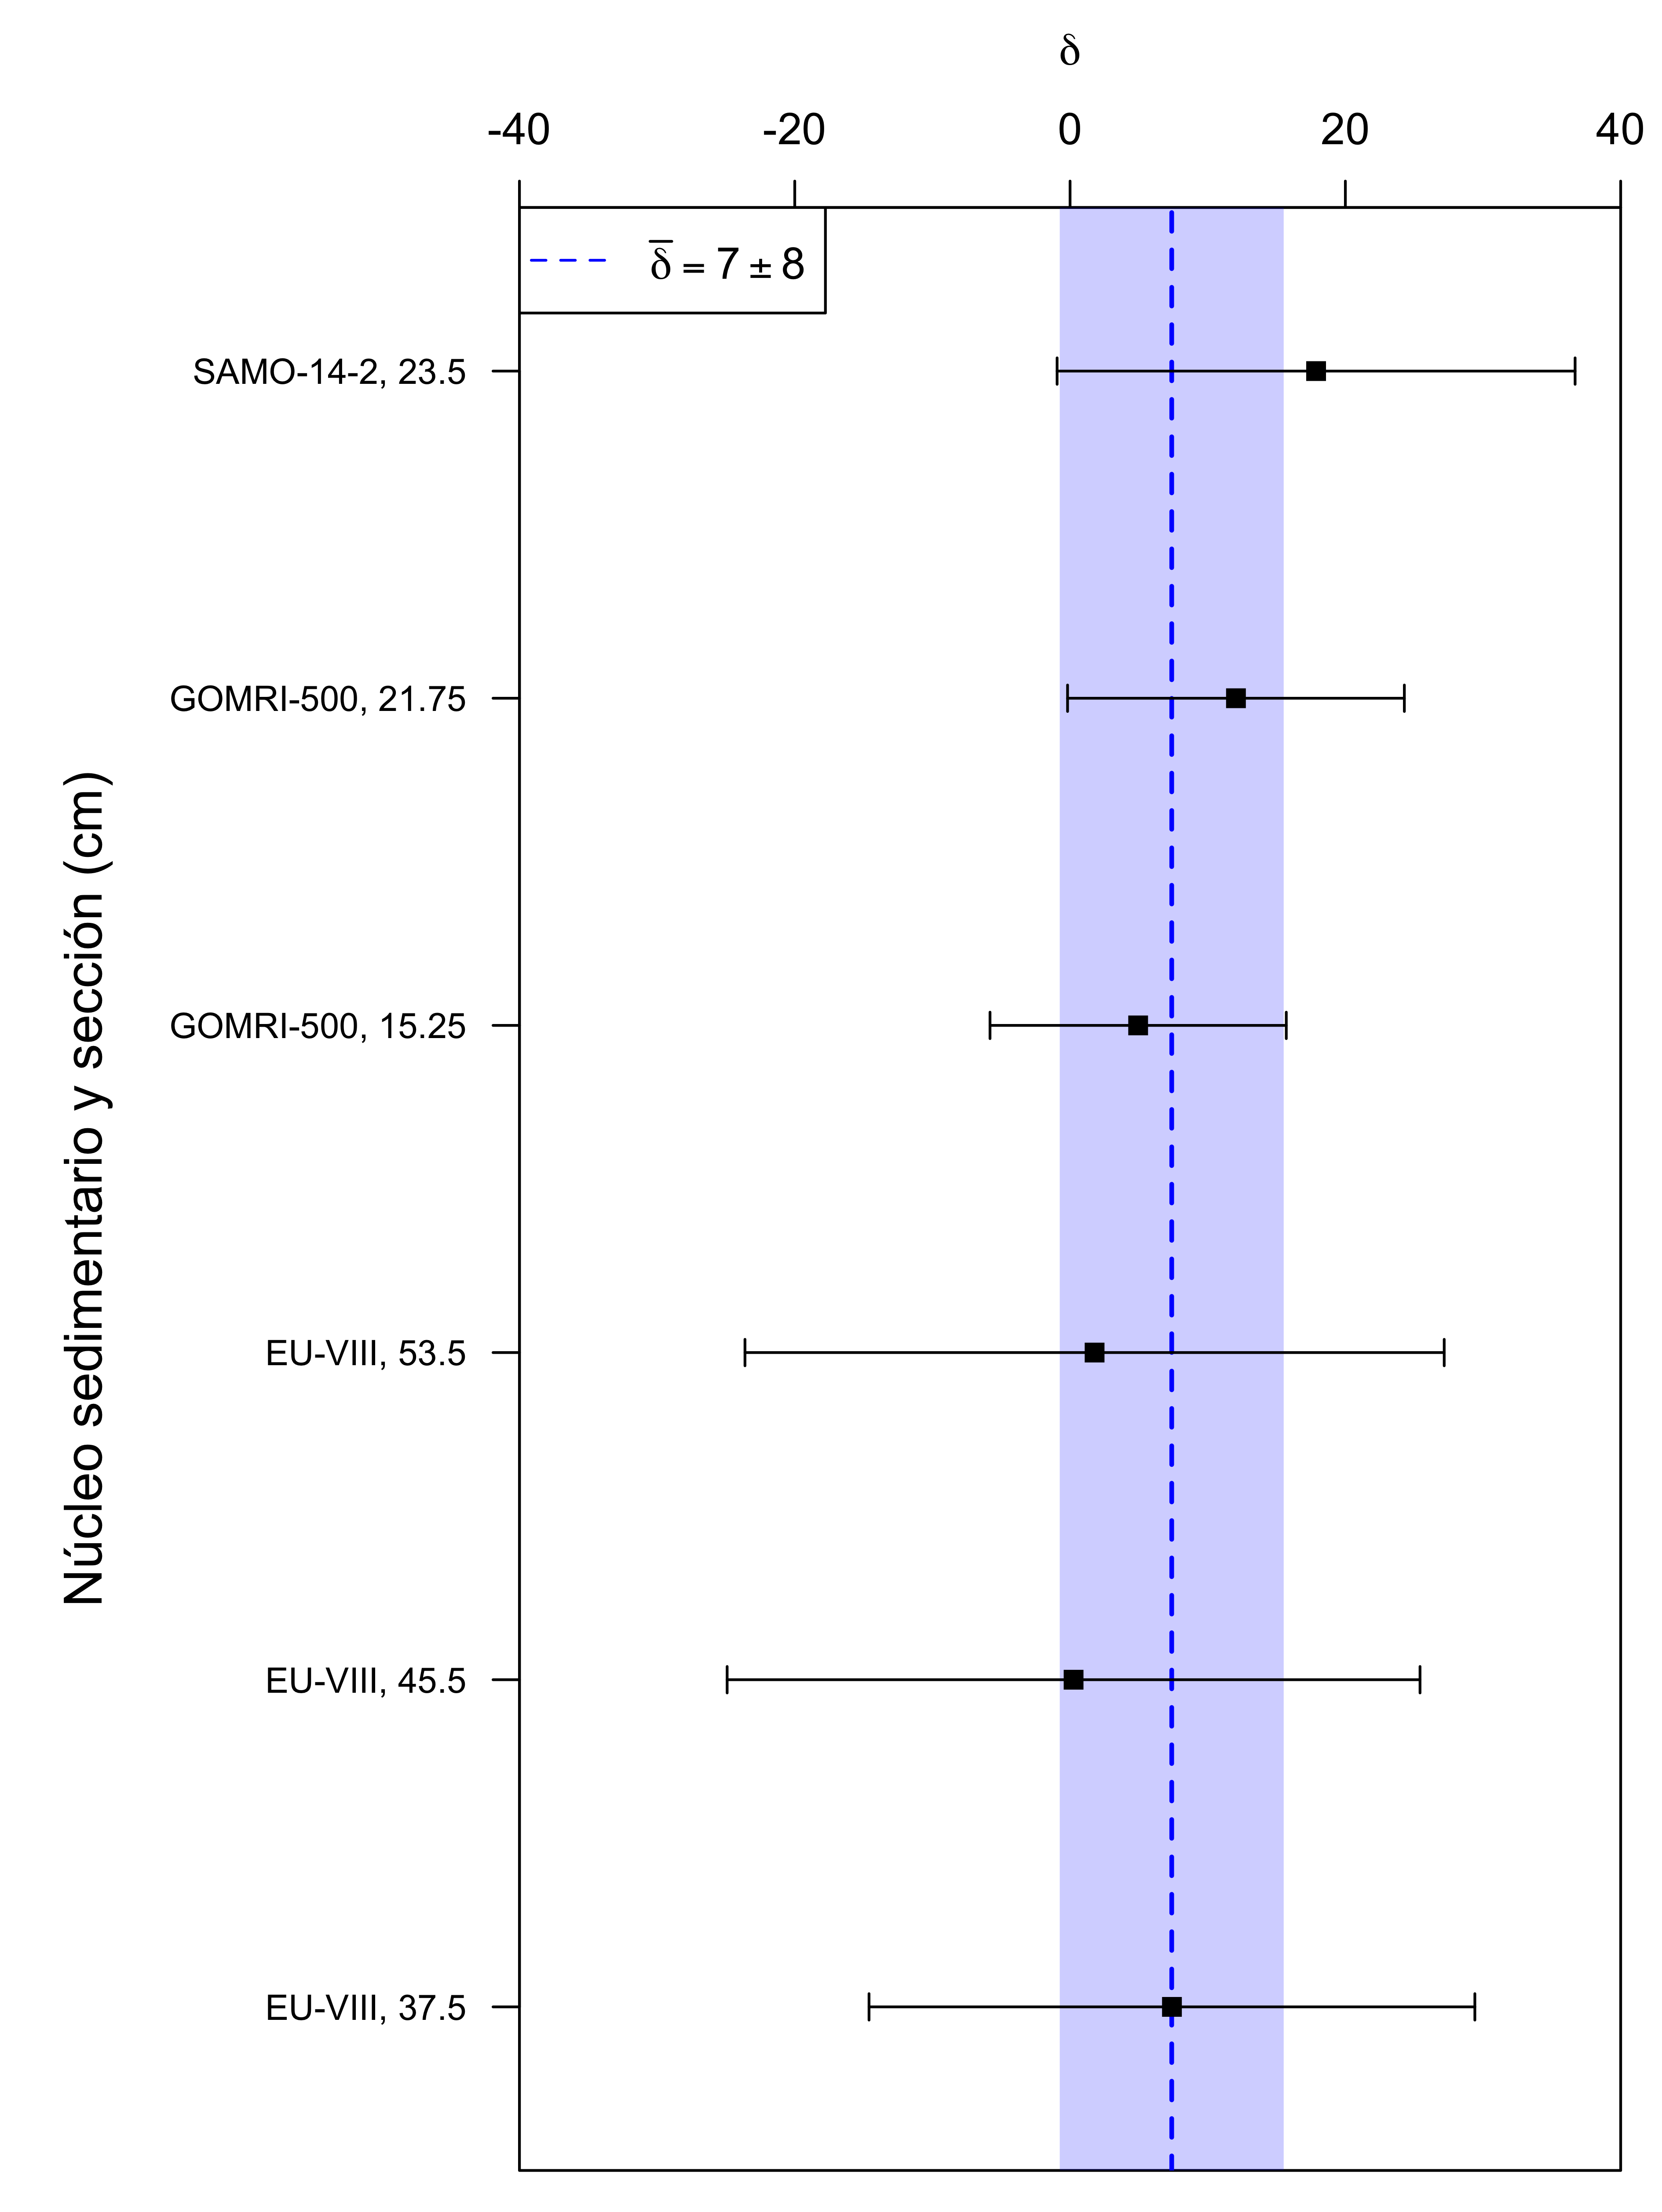
\includegraphics[width=0.9\textwidth]{Imagenes/Grafica_Delta_210Pb_214Pb-2.png}
\caption{Diferencia porcentual $\delta$ de los valores de la actividad específica de \PbCero\, respecto a la actividad específica de \PbCuatro\, para las secciones que se encuentran en equilibrio de los núcleos sedimentarios EU-VIII, GOMRI-500 y SAMO-14-2 asumiendo una composición corregida.}\label{Fig-DiffPorcentualEquilibrio}
\end{figure}
\newpage
	\section{Fechado}\label{Seccion-Fechado}
Las actividades de referencia y corregidas, y las profundidades a partir de las cuales se asumió el equilibrio secular, fueron utilizadas para establecer los modelos de edad con el modelo CF (Sección \ref{SubSec-Fechado}). En todos los casos, y como es conocido \cite{SANCHEZCABEZA2012183}, las incertidumbres de los modelos de edad crecen con la profundidad. Los modelos de edad y las diferencias porcentuales para los núcleos sedimentarios con composición corregida y composición no corregida se muestran en las Figuras \ref{ModeloEdad-EUVIII}, \ref{ModeloEdad-GOMRI500}, \ref{ModeloEdad-PCm}, \ref{ModeloEdad-LTAF}, \ref{ModeloEdad-SAMO} y \ref{ModeloEdad-TEHUAXII}, y los promedios de las diferencias porcentuales en la Tabla \ref{Tabla-DiferenciasPorcentualesFechado}. 
\\
\\
La Tabla \ref{Tabla-DiferenciasPorcentualesFechado} muestra la variabilidad de las diferencias porcentuales promedios de las eficiencias y de las masas, así como las diferencias porcentuales promedio en los modelos de edad. 
\\
\\
De acuerdo con la mínima corrección en eficiencia realizada, el núcleo PCm mostró modelos de edad prácticamente coincidentes con una diferencia porcentual entre los modelos de 0.1 \% (Figura \ref{ModeloEdad-PCm}, Tabla \ref{Tabla-DiferenciasPorcentualesFechado}). En el otro extremo, si bien la mayor corrección promedio fue para el núcleo GOMRI-500, su desviación promedio en el modelo de edad fue de las más bajas (3 $\pm$ 2 \%). En esta misma dirección, la corrección del modelo de edad más fuerte fue para el núcleo EU-VIII (22 $\pm$ 2 \%), que sí mostró una corrección de eficiencia importante (12 \%). Es pues claro que la corrección de eficiencia no es la única variable que explica la variación en los modelos de edad. 
\\
\\
Por otra parte, en el modelo de fechado de Flujo Constante, el fechado corregido $t$ de una sección es 
\begin{equation}
t(i) =  \dfrac{1}{\lambda}\,\ln\left(\dfrac{\sum_{j=1}^\infty A_{j, \text{corr}}\, m_j}{ \sum_{j=i+1}^\infty A_{j, \text{corr}}\, m_j}\right) = 
\dfrac{1}{\lambda}\,\ln\left(\dfrac{\sum_{j=1}^\infty \dfrac{\epsilon_{j, \text{ref}}}{\epsilon_{j, \text{corr}}} A_{j, \text{ref}}\, m_j}{ \sum_{j=i+1}^\infty \dfrac{\epsilon_{j, \text{ref}}}{\epsilon_{j, \text{corr}}} A_{j, \text{ref}}\, m_j}\right).
\end{equation}
Si las eficiencias de referencia $\epsilon_{j, \text{ref}}$ y corregida $\epsilon_{j, \text{corr}}$ de la sección $j$ son constantes a lo largo del núcleo, entonces $A_{j, \text{corr}} \propto A_{j, \text{ref}}$ para todo valor de $j$ (Ecuación \ref{Eq-ActividadCorregida}) y el fechado $t$ no se ve afectado.
\\
\\
Por lo tanto, es posible que las diferencias en los modelos de edad no se deban tanto a la corrección de eficiencia sino a su variabilidad (es decir, que no se cumpla la hipótesis de una corrección de eficiencia constante). Como se observa en la Tabla \ref{Tabla-DiferenciasPorcentualesFechado}, la variabilidad de la corrección de eficiencia también influye en la corrección del fechado, pero no es la única variable relevante. El fechado con el modelo CF también requiere el conocimiento de las masas, que presentan una fuerte variabilidad como se observa en la Tabla \ref{Tabla-DiferenciasPorcentualesFechado}. Por lo tanto, es la combinación compleja de los valores absolutos y variabilidades de las masas y las eficiencias las que determinan la desviación final del modelo de edad corregido y, por ello, dependerá de cada caso concreto. Esta conclusión acentúa la necesidad de disponer de actividades absolutas lo más próximas a las reales y una medida confiable de la masa real de cada sección.
\begin{figure}[h]
\centering
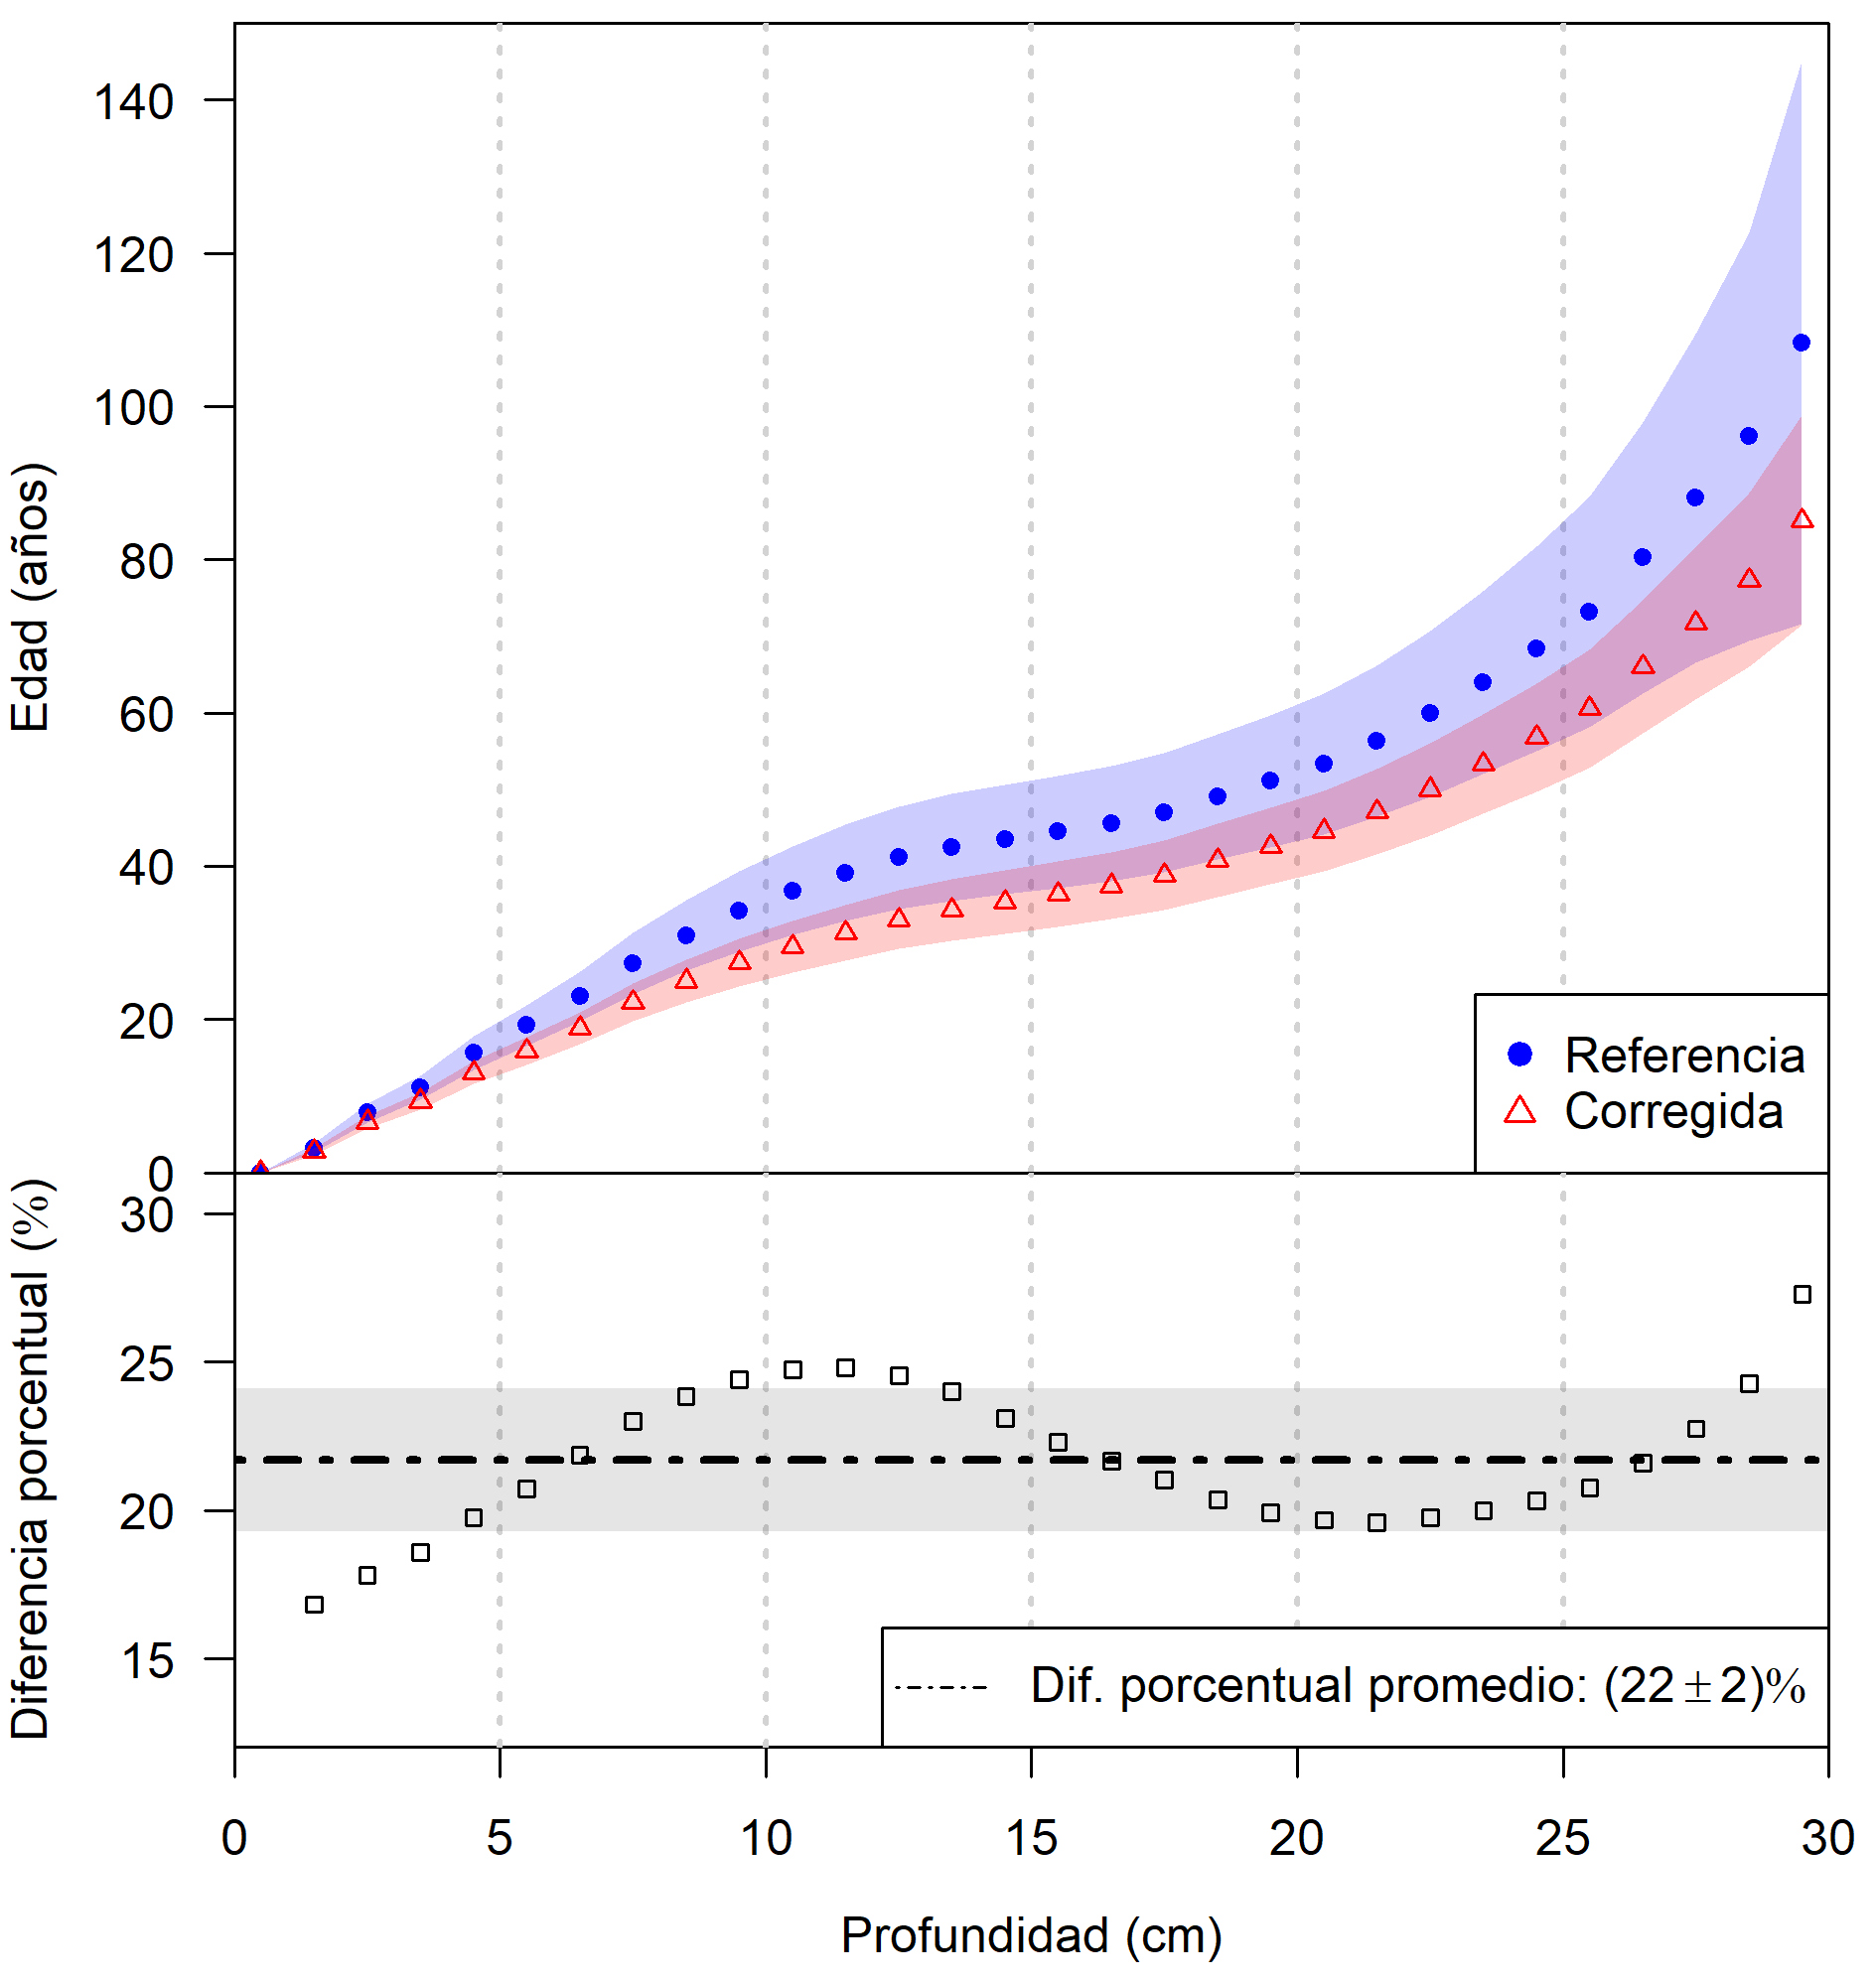
\includegraphics[width=0.9\textwidth]{Imagenes/EUVIII_1.png}
\caption{Modelo de edad del núcleo \textbf{EU-VIII} para la composición de referencia y la composición corregida. En la parte inferior se muestra la diferencia porcentual respecto a composición de referencia.}\label{ModeloEdad-EUVIII}
\end{figure}

\begin{figure}[h]
\centering
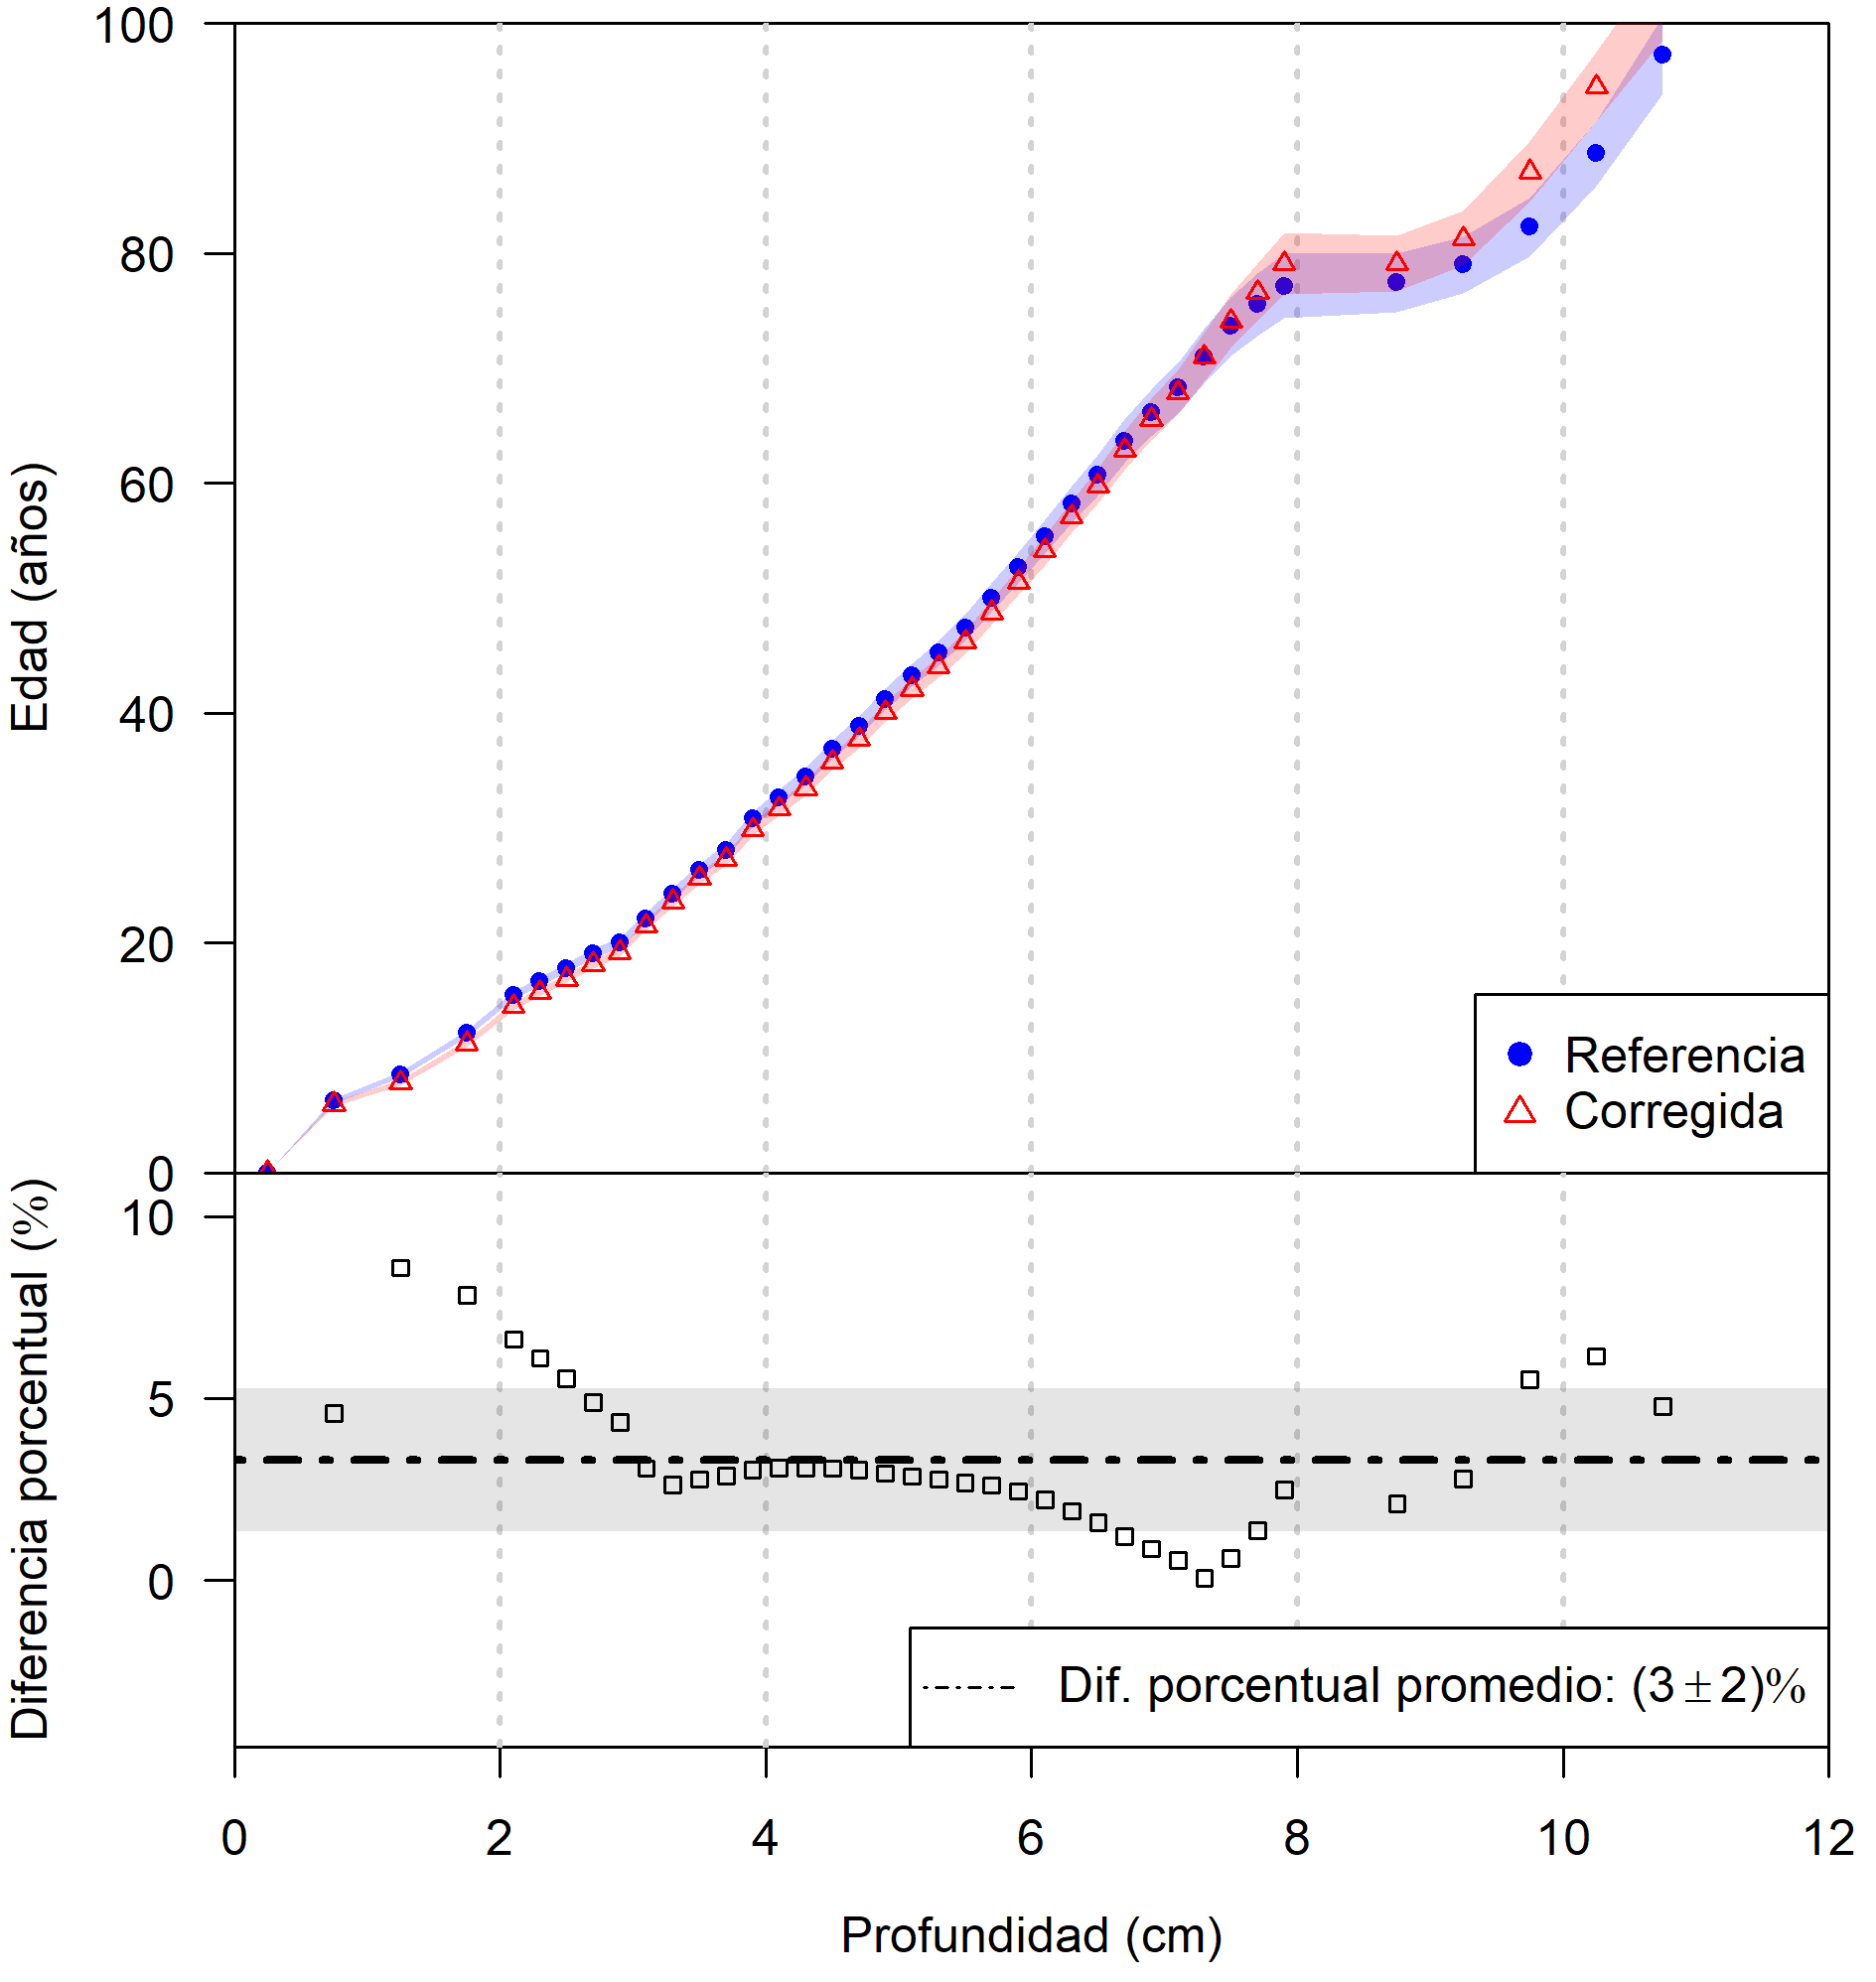
\includegraphics[width=0.9\textwidth]{Imagenes/GOMRI500_1.png}
\caption{Modelo de edad del núcleo \textbf{GOMRI-500} para la composición de referencia y la composición corregida. En la parte inferior se muestra la diferencia porcentual respecto a composición de referencia.}\label{ModeloEdad-GOMRI500}
\end{figure}

\begin{figure}[h]
\centering
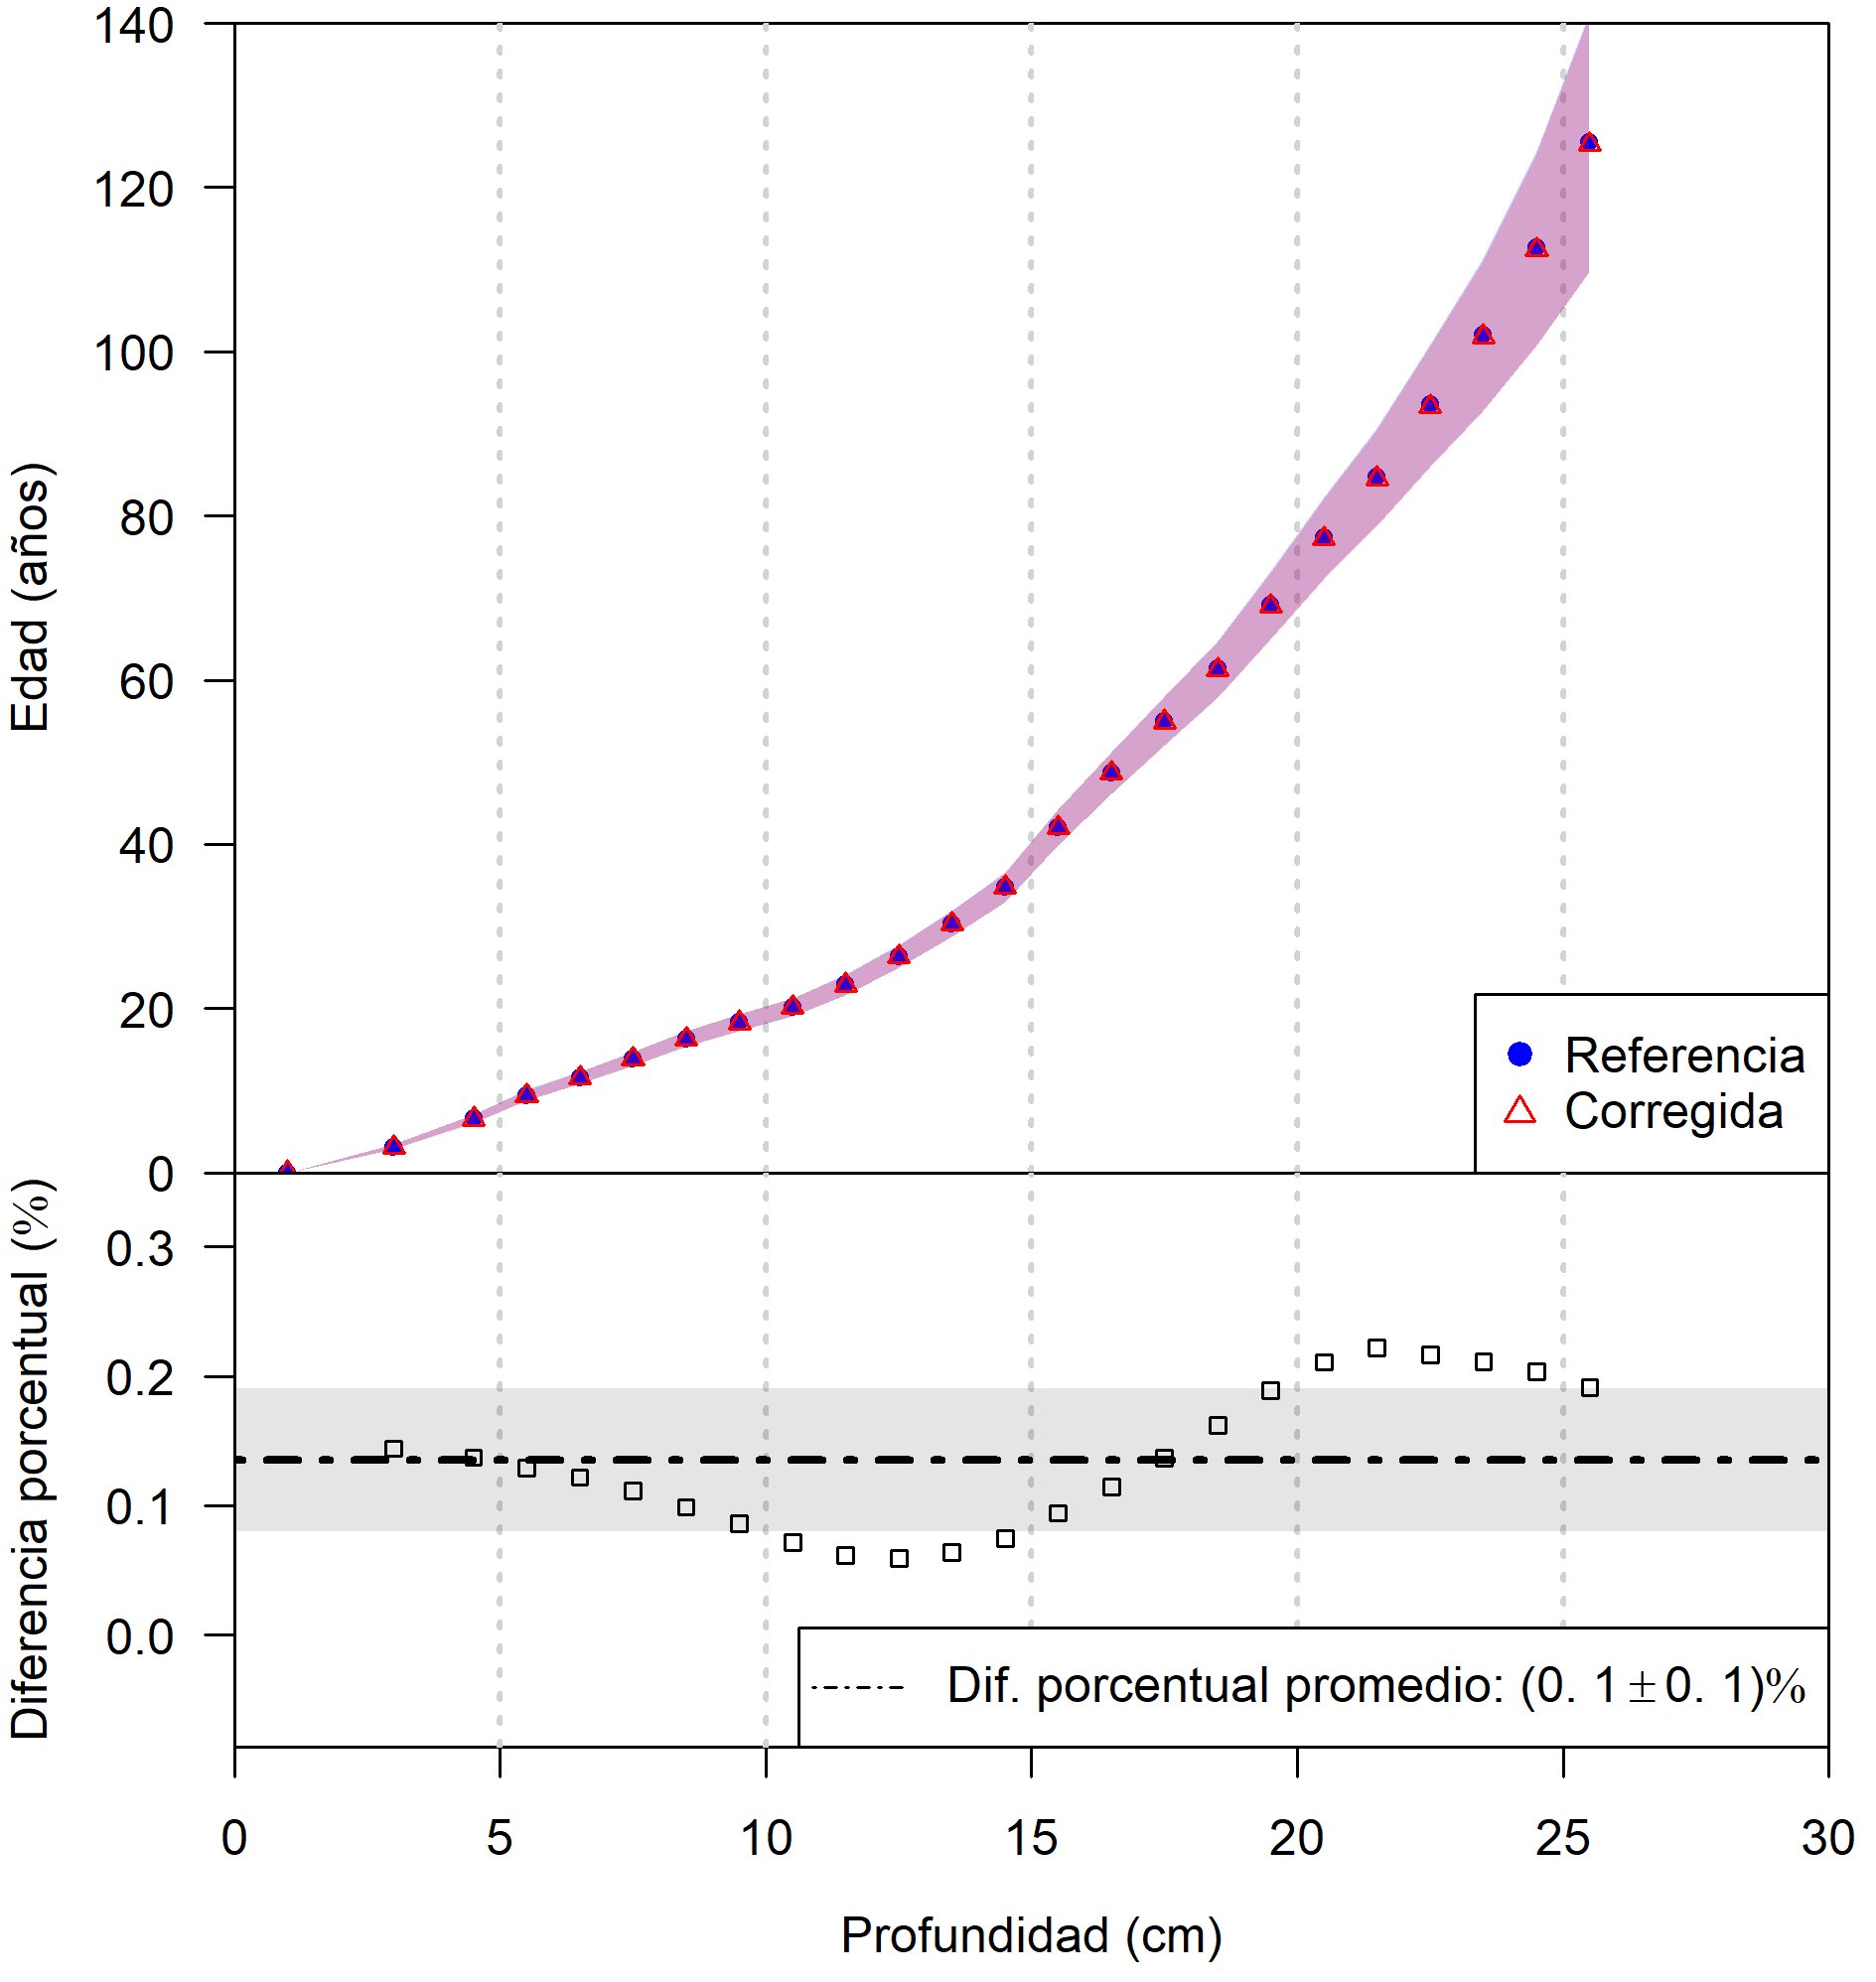
\includegraphics[width=0.9\textwidth]{Imagenes/PCm_1.png}
\caption{Modelo de edad del núcleo \textbf{PCm} para la composición de referencia y la composición corregida. En la parte inferior se muestra la diferencia porcentual respecto a composición de referencia.}\label{ModeloEdad-PCm}
\end{figure}

\begin{figure}[h]
\centering
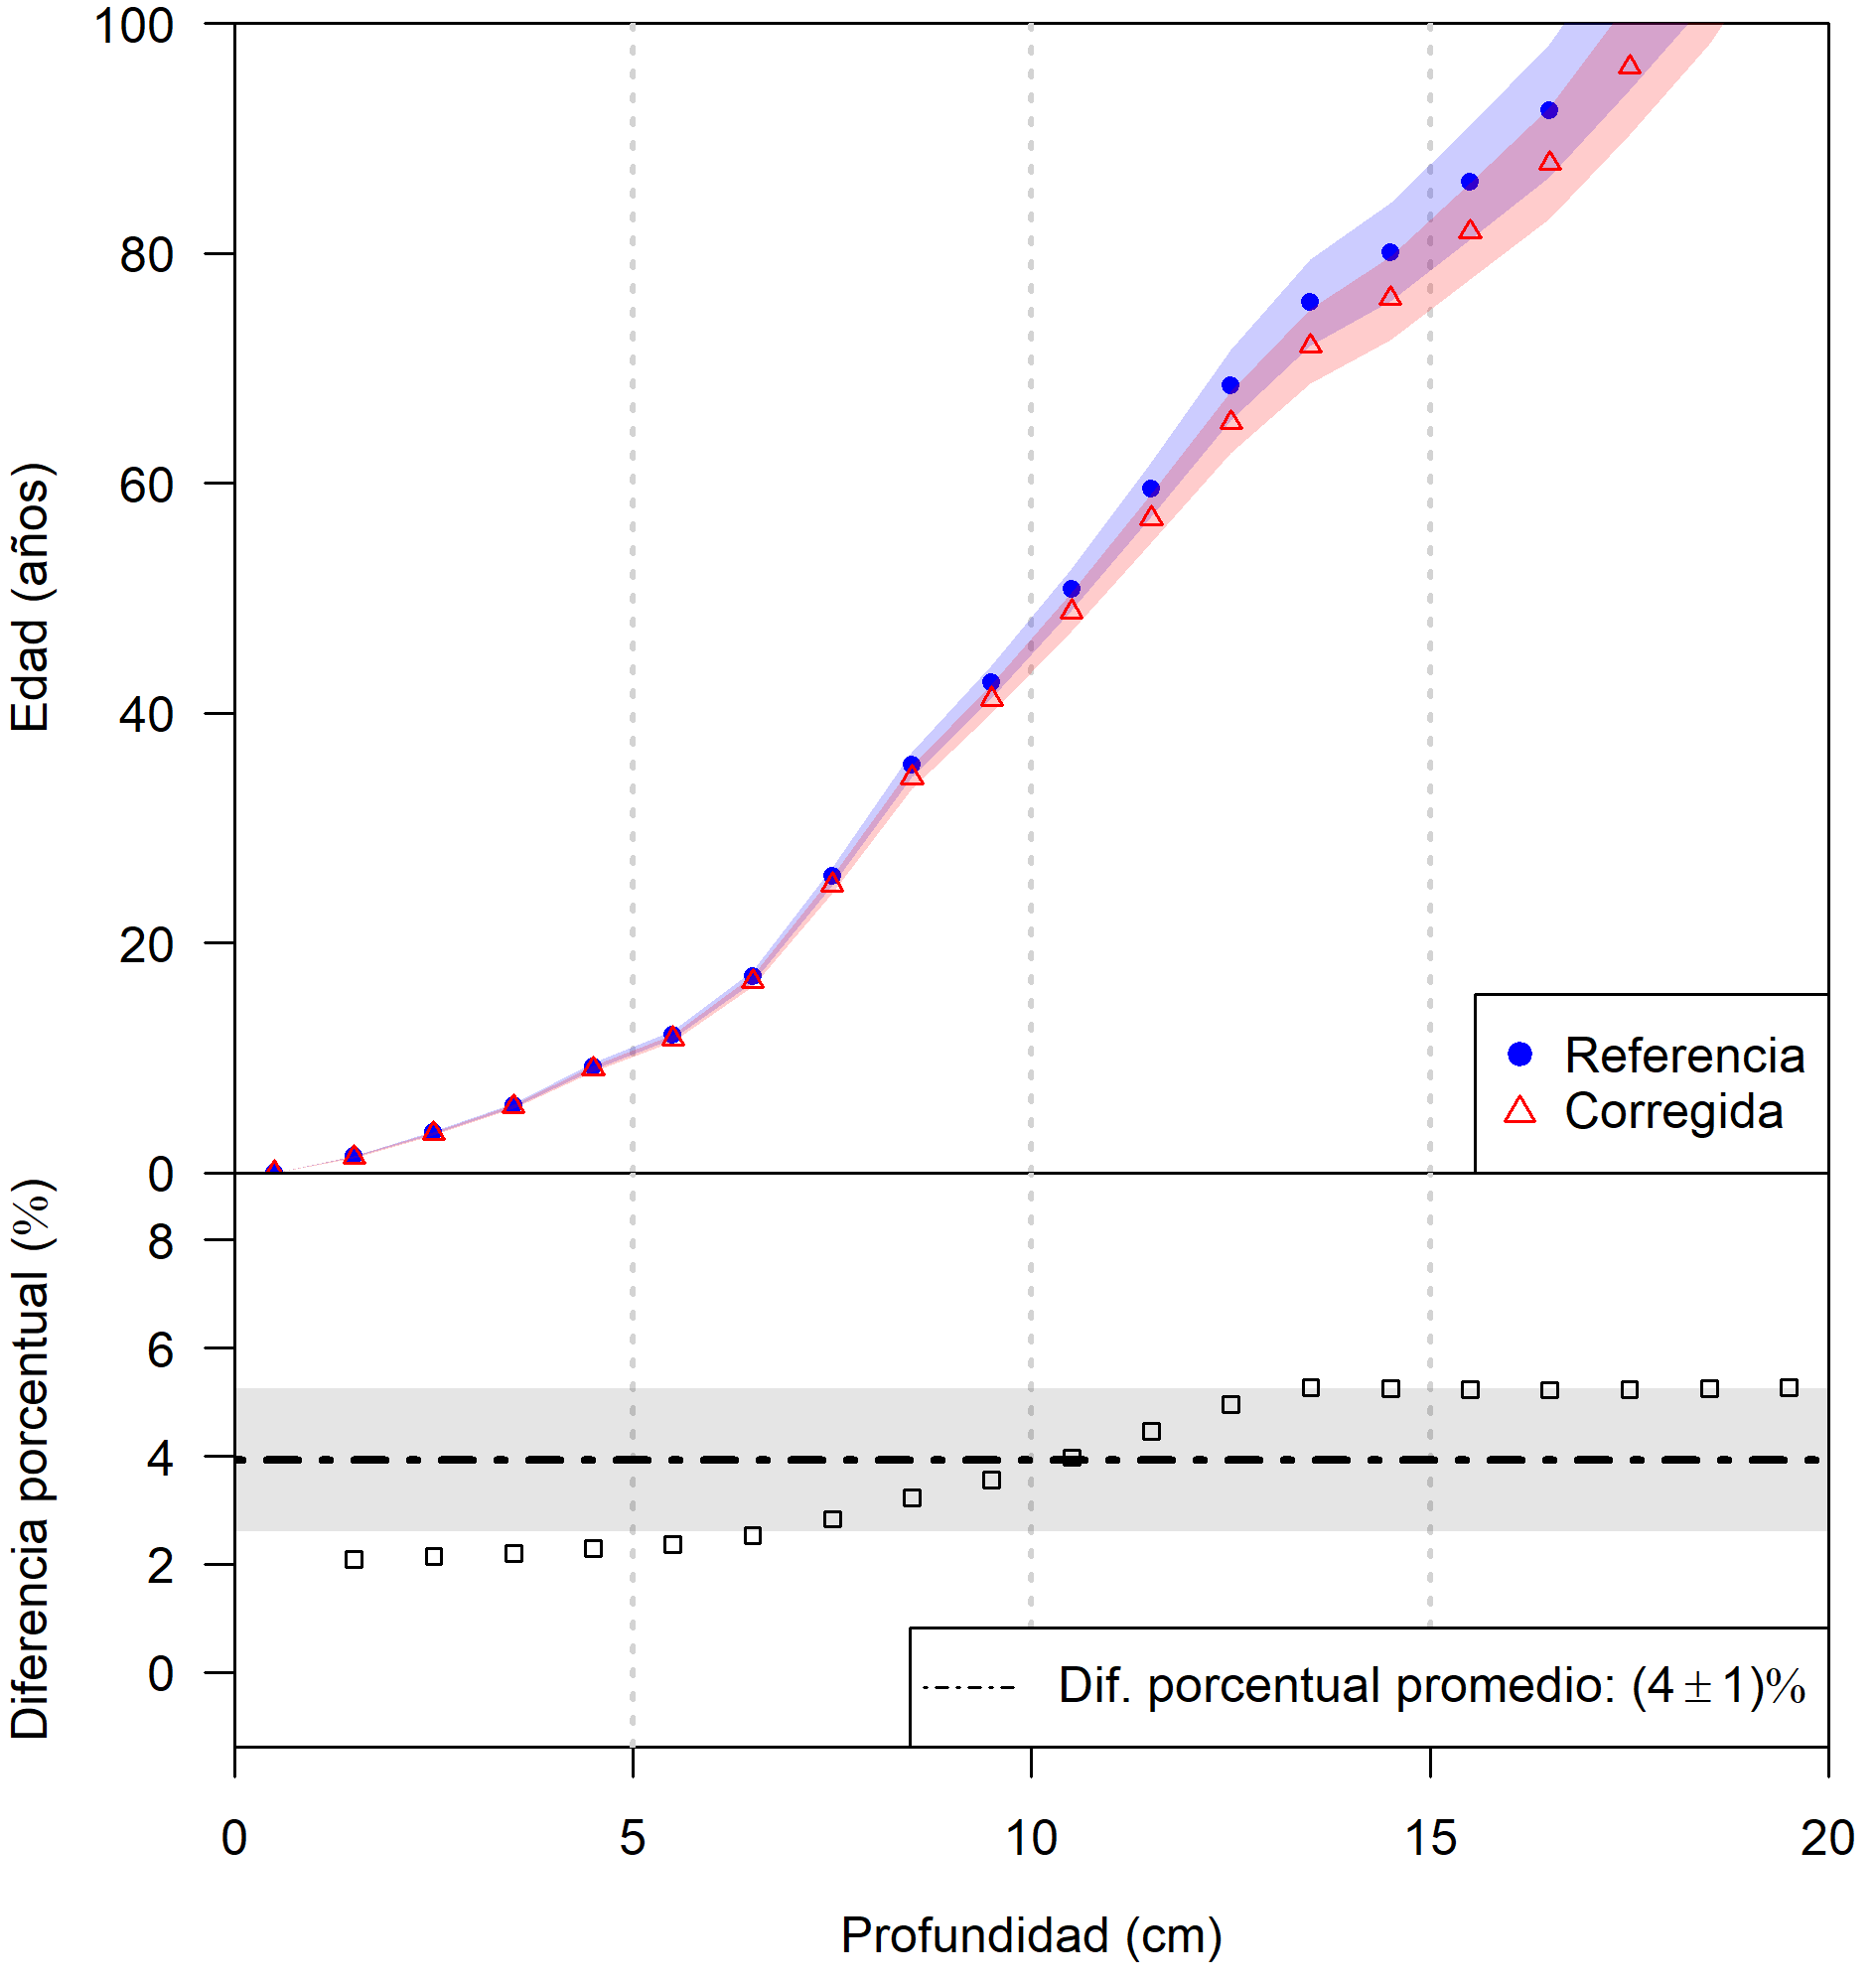
\includegraphics[width=0.9\textwidth]{Imagenes/LTAF_1.png}
\caption{Modelo de edad del núcleo \textbf{LTAF} para la composición de referencia y la composición corregida. En la parte inferior se muestra la diferencia porcentual respecto a composición de referencia.}\label{ModeloEdad-LTAF}
\end{figure}

\begin{figure}[h]
\centering
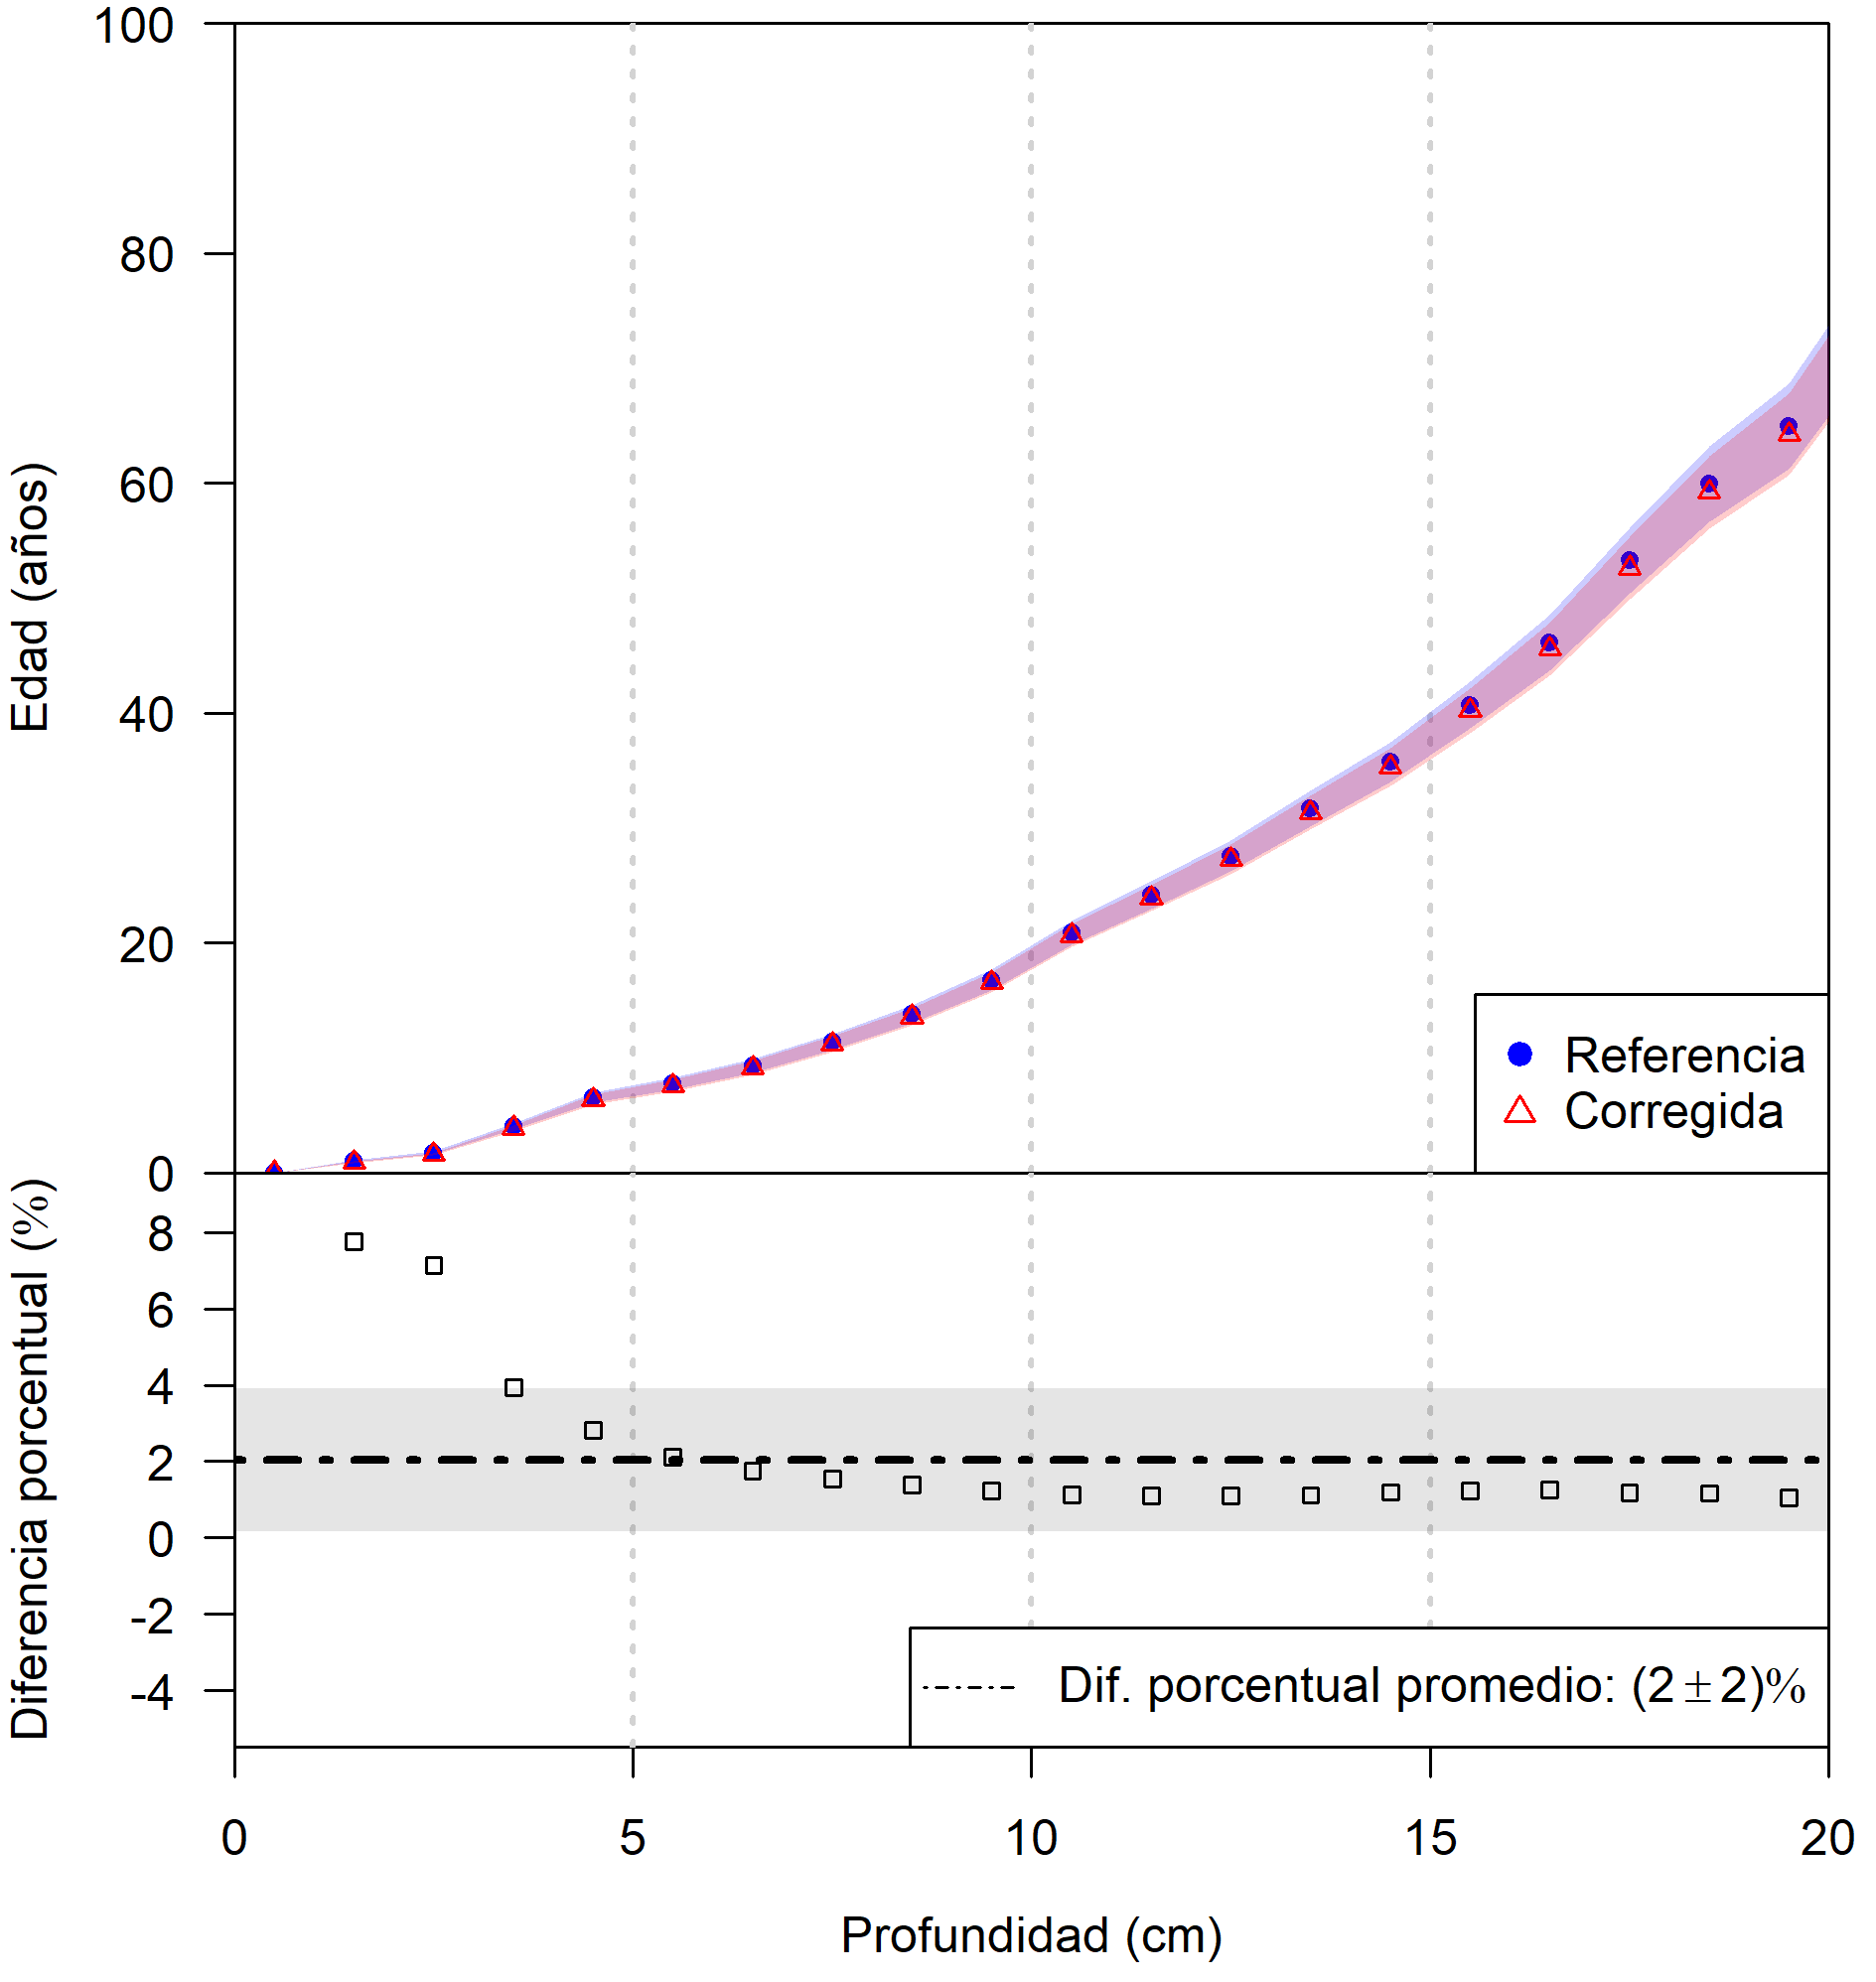
\includegraphics[width=0.9\textwidth]{Imagenes/SAMO142_1.png}
\caption{Modelo de edad del núcleo \textbf{SAMO-14-2} para la composición de referencia y la composición corregida. En la parte inferior se muestra la diferencia porcentual respecto a composición de referencia.}\label{ModeloEdad-SAMO}
\end{figure}

\begin{figure}[h]
\centering
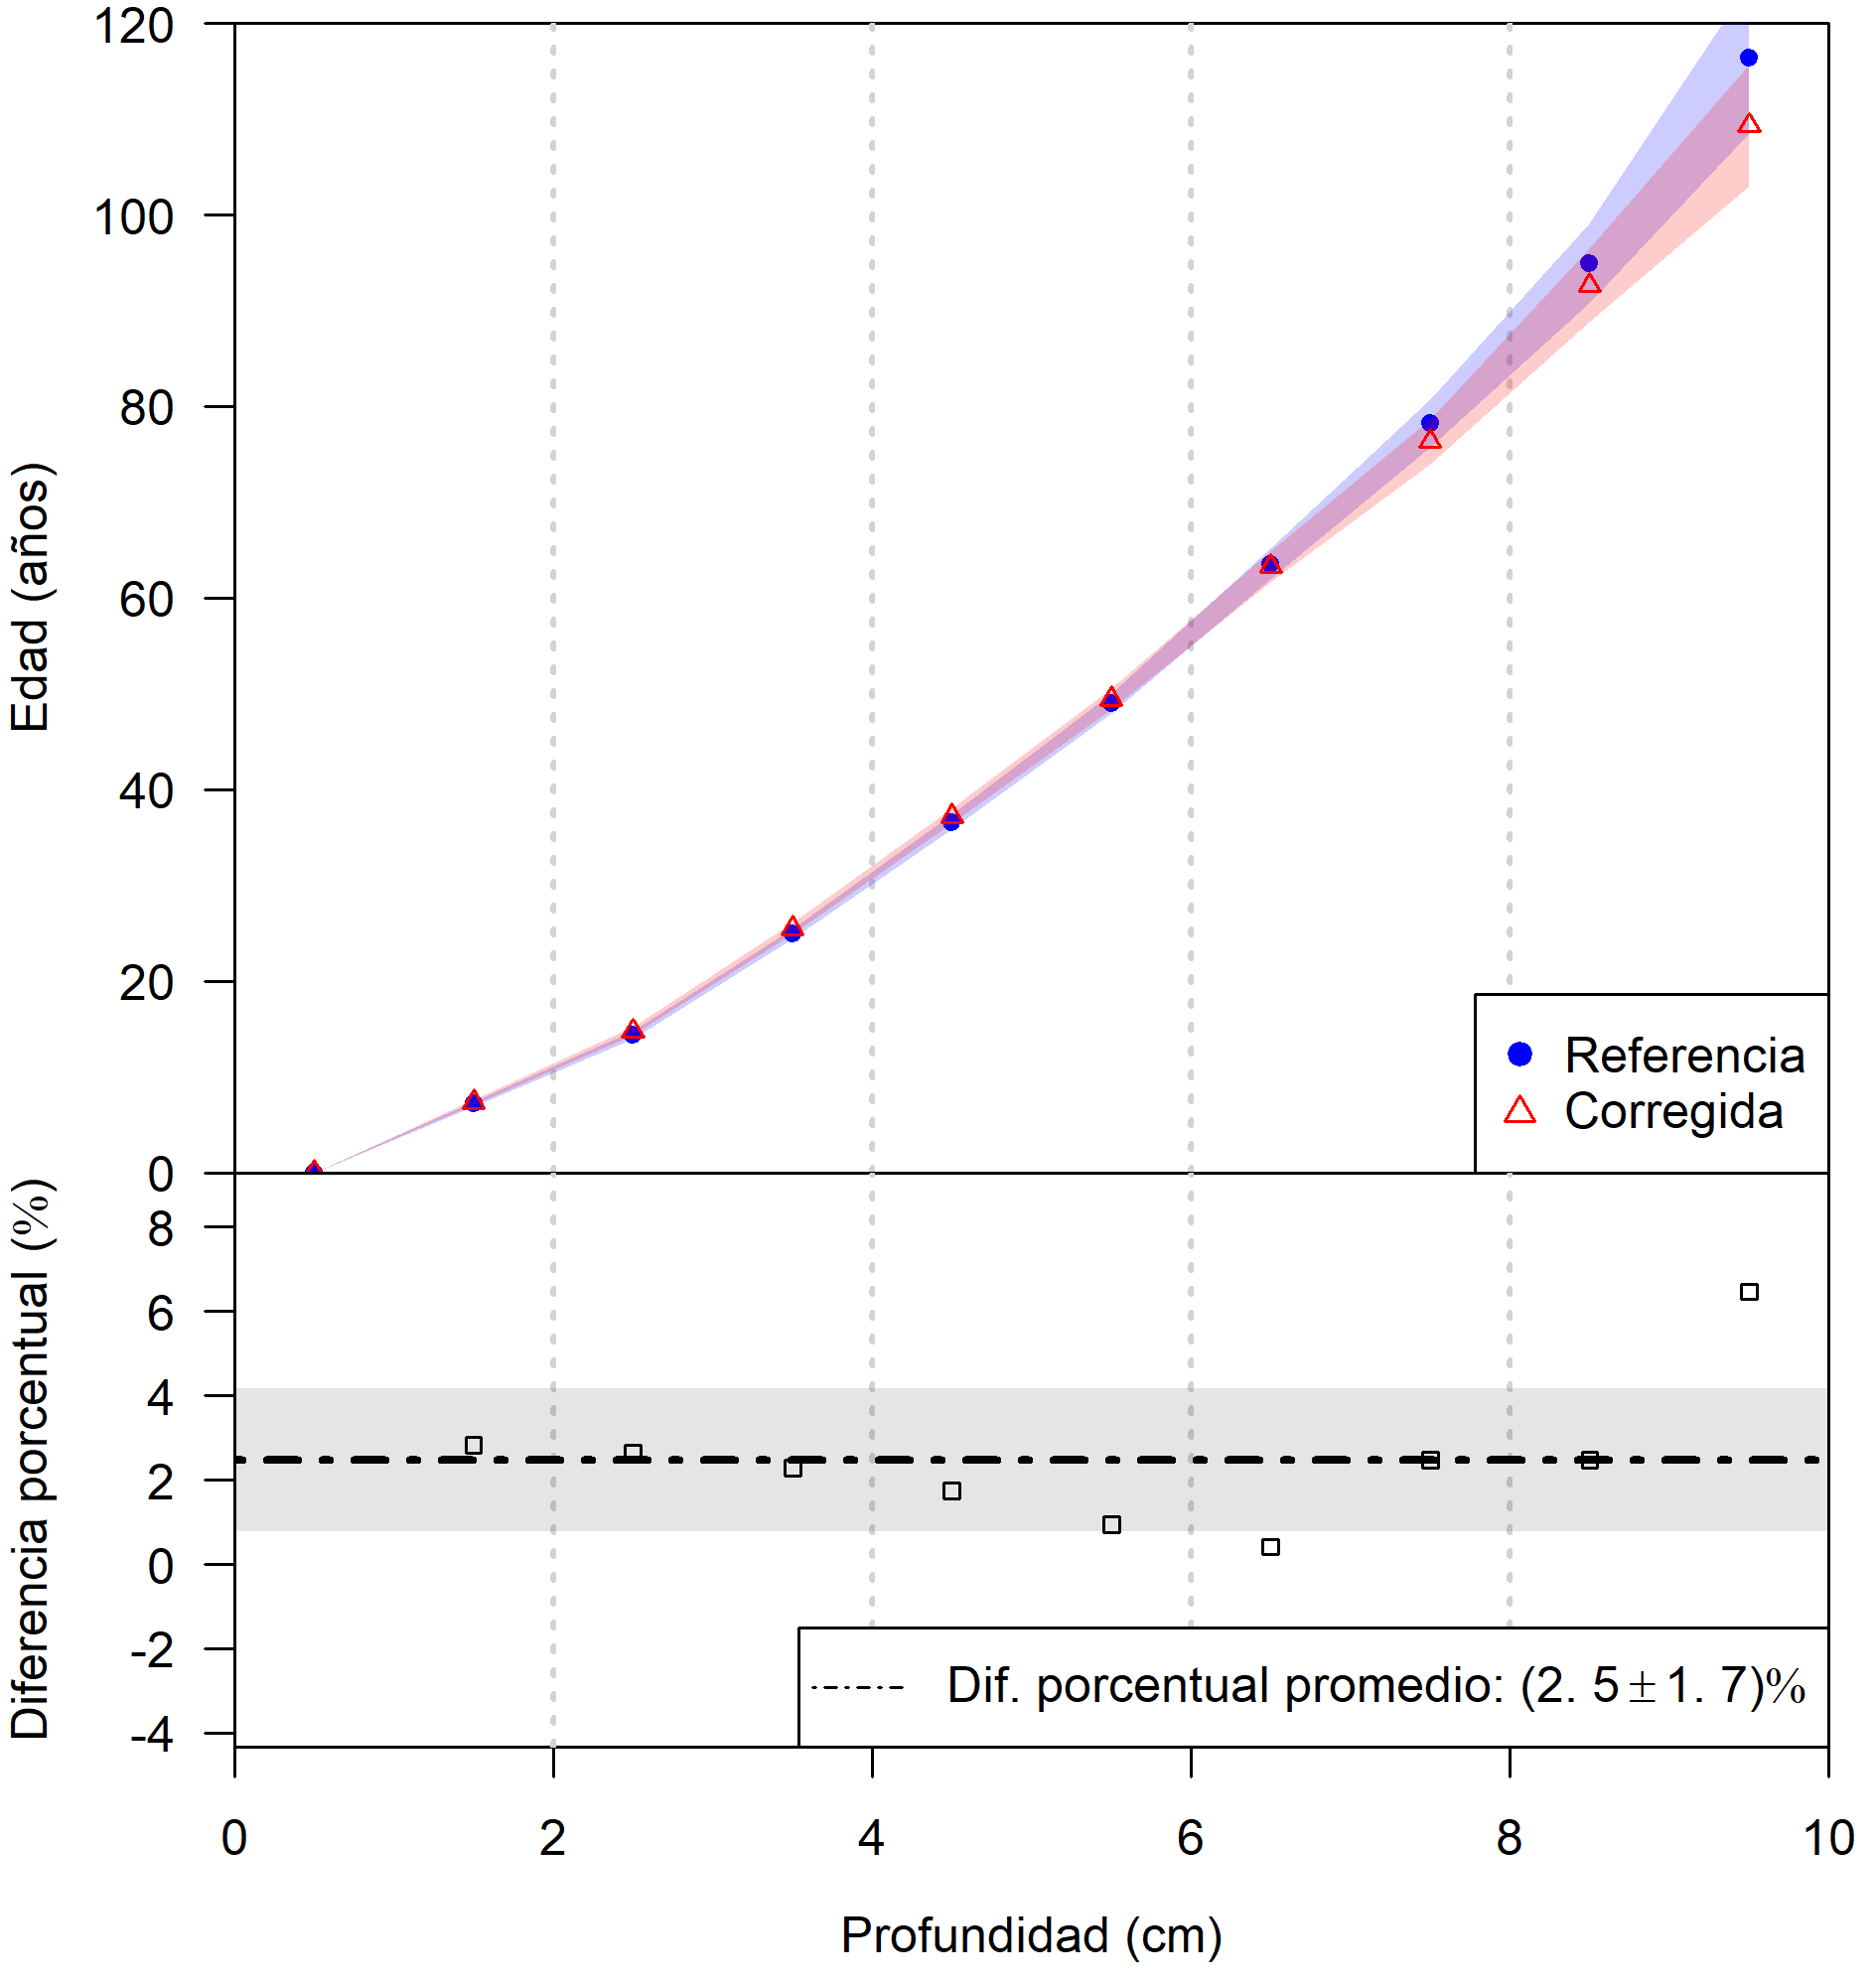
\includegraphics[width=0.9\textwidth]{Imagenes/TEHUA_1.png}
\caption{Modelo de edad del núcleo \textbf{TEHUA-XII} para la composición de referencia y la composición corregida. En la parte inferior se muestra la diferencia porcentual respecto a composición de referencia.}\label{ModeloEdad-TEHUAXII}
\end{figure}

\begin{table}[h]
\centering
\caption{Variabilidad en la diferencia porcentual promedio de las eficiencias para una energía de 46.54 keV (Tabla \ref{Tabla-Eficiencias}), variabilidad de las masas de las secciones a lo largo del núcleo y diferencia porcentual promedio entre los modelos de edad.}\label{Tabla-DiferenciasPorcentualesFechado}
\begin{tabular}{|c|c|c|c|} \hline 
\rowcolor{Blue2} & & & \\
\rowcolor{Blue2} Núcleo 			& $\dfrac{\bigtriangleup \epsilon}{\overline{\epsilon}} \times 100$ 	& $\dfrac{\bigtriangleup m}{\overline{m}} \times 100$ & Dif. promedio en modelo de edad \\
\rowcolor{Blue2} & & & \\ \hline
\rowcolor{Blue1} GOMRI-500 	& $6$ \% 								& 42 \% 			& $3\pm 2$ \% \\ 
\rowcolor{Blue1} TEHUA-XII 	&  $25$ \% 								& 16 \% 			&$2.5 \pm 1.7$ \% \\ 
\rowcolor{Blue1}LTAF 			& $33$ \% 								& 44 \% 			&$4\pm 1$ \%\\ 
\rowcolor{Blue1}PCm 				& $47$ \% 							& 17 \% 			&$0\pm 0$ \% \\
\rowcolor{Blue1} EU-VIII 			&	$8$ \% 								& 16 \% 			&$22\pm 2$ \% \\
\rowcolor{Blue1} SAMO-14-2 	&	$22$ \% 						& 32 \% 			&$2\pm 2$ \% \\
\hline
\end{tabular}
\end{table}